%%%%%%%%%%%%%%%%%%%%%%%%%%%%%%%%%%%%%%%%%%%%%%%%%%%%%%%%%%%%%%%%%%%%%%%%%%
%% 
%% Bachelor Thesis Template of the PRG Group
%%
%%%%%%%%%%%%%%%%%%%%%%%%%%%%%%%%%%%%%%%%%%%%%%%%%%%%%%%%%%%%%%%%%%%%%%%%%%
\documentclass[12pt,twoside,a4paper,fleqn,bibliography=totocnumbered]{report}

% some often used and useful packages (others can be added if necessary)
\usepackage{latexsym}
\usepackage[utf8]{inputenc}
\usepackage{subfigure}
\usepackage{graphicx}
\usepackage{amsmath,amssymb}
\usepackage{algorithm}
\usepackage{amsfonts}
\usepackage{multirow}
\usepackage{xspace}
\usepackage{booktabs}
\usepackage{array}
\usepackage{pifont}
\usepackage{psfrag}
\usepackage{epsfig}
\usepackage{bm}
\usepackage{wasysym}
\usepackage[table]{xcolor}
\usepackage{setspace}
\usepackage{framed}
\usepackage{float,pdflscape}
\usepackage{url}
\usepackage{color}
\usepackage{minted}
\usepackage{algpseudocode}
\usepackage[margin=1.1in,bindingoffset=.2in]{geometry} 
\usepackage{longtable}
\usepackage{tabularx}   % For better table formatting
\usepackage{multicol}    % For multi-column layouts

% Set global table parameters for more compact tables
\renewcommand{\arraystretch}{0.95}  % More compact rows
\setlength{\tabcolsep}{4pt}         % Tighter column spacing

% Add consistent notation macros for vectors, matrices, and number sets
\newcommand{\vect}[1]{\boldsymbol{#1}}
\newcommand{\mat}[1]{\mathbf{#1}}
\newcommand{\R}{\mathbb{R}}
\newcommand{\Z}{\mathbb{Z}}
\newcommand{\C}{\mathbb{C}}

\onehalfspacing



\begin{document}


% frontmatter
\input title.tex
\pagenumbering{roman}
\setcounter{page}{1}
\cleardoublepage
\begin{abstract}
This study investigates the optimization of the student transportation network for the Izmir Institute of Technology (IZTECH) using graph-based methodologies. The primary objective is to minimize total transportation costs while adhering to vehicle capacity constraints (10-50 students per bus) for a synthetically generated dataset of approximately 2000 student locations across Izmir.
The study systematically evaluates various graph construction techniques, including Complete Graph, Delaunay Triangulation, Gabriel Graph, and K-Nearest Neighbors (KNN) graph, in conjunction with three distinct clustering algorithms: Spectral Clustering, the Leiden Algorithm, and Multi-view Anchor Graph-based Clustering (MVAGC). Furthermore, the impact of a K-Nearest Neighbor (KNN) distance-based outlier detection method on overall network efficiency is assessed.
Experimental results demonstrate that sparse graph representations are crucial for computational tractability and improved routing solutions compared to a complete graph. The combination of Gabriel Graph construction with the Leiden algorithm and KNN distance-based outlier detection yielded the most significant improvements, achieving the lowest total transportation cost (110,364.09 TL) and the fewest number of required bus routes (60). This represents an approximate 11.0\% cost reduction compared to the baseline complete graph approach with Leiden clustering.
The findings confirm that appropriate data preprocessing, sparse graph representation, and effective clustering algorithms are essential for optimizing transportation networks. Specifically, the Gabriel graph combined with Leiden clustering and outlier removal offers a robust and efficient strategy for IZTECH to enhance its student transportation system.
\end{abstract}















%\cleardoublepage
\input acknowledgments.tex % delete this and next line if not applicable
%\cleardoublepage
\tableofcontents
\cleardoublepage
\pagenumbering{arabic}
\setcounter{page}{1}

% The major parts 
\chapter{Introduction}
\label{ch:introduction}

\section{Motivation}
\label{sec:intro_motivation}
Efficient transportation systems are fundamental to the vitality and accessibility of university campuses, profoundly impacting student life, operational sustainability, and environmental stewardship \cite{dell2016campus, guido2017sustainable}. For an institution such as the Izmir Institute of Technology (IZTECH), which serves a student population of approximately 5500~\cite{iztech_info} spread across the expansive metropolitan area of Izmir, the logistical complexities are considerable. IZTECH, a key technological university, plays a significant role in the educational and research landscape of the region, making the well-being and accessibility for its students a priority. The challenge of designing an optimized transportation network for IZTECH students is multifaceted. It involves not only managing substantial operational costs related to fuel consumption and vehicle maintenance but also enhancing the daily commute for a large, geographically dispersed student body. The inherent difficulties include optimizing routes with fluctuating demand, developing computationally feasible solutions for a large-scale network, and addressing imperfections in real-world data \cite{kaviani2019smart, saberi2017models}. Therefore, optimizing the student transportation network is crucial for improving student experience, ensuring equitable access to education, and promoting the overall efficiency of the university's operations. This thesis endeavors to address these challenges by systematically applying and rigorously evaluating graph theory principles and advanced clustering algorithms to architect an optimized bus routing system tailored for IZTECH students.

\section{State-of-the-Art}
\label{sec:intro_sota}
The problem of vehicle routing and transportation network optimization has been extensively studied, with a rich body of literature focusing on various methodologies \cite{toth2014vehicle}. Graph theory provides a natural and powerful framework for modeling transportation networks, where locations are represented as vertices and travel segments as edges \cite{tarapata2019graph}. Within this framework, several key areas of research are pertinent to this thesis.

Graph construction techniques are crucial for creating accurate and computationally manageable representations of transportation networks. While complete graphs offer comprehensive connectivity, their $O(N^2)$ complexity is prohibitive for large datasets. Consequently, sparse graph construction methods such as K-Nearest Neighbors (KNN) graphs, Delaunay Triangulation, and Gabriel Graphs are widely adopted. These methods aim to preserve essential connectivity, particularly local spatial relationships, while significantly reducing the number of edges, thereby enhancing computational efficiency (see Chapter~\ref{ch:basics}). The choice of graph representation profoundly influences the subsequent analysis and the quality of the derived solutions.

Once a graph representation is established, clustering algorithms are employed to partition the network into manageable sub-units, which in this context correspond to potential bus routes. Graph clustering, or community detection, seeks to identify groups of vertices that are densely connected internally while being sparsely connected to the rest of the graph. Prominent algorithms in this domain include Spectral Clustering, which utilizes the eigenspectrum of graph Laplacian matrices to find optimal cuts (see Chapter~\ref{ch:basics}). The Leiden algorithm, an improvement over the Louvain method, is another state-of-the-art technique known for its ability to find well-connected communities by optimizing modularity~\cite{leiden}. More advanced methods like Multi-view Anchor Graph-based Clustering (MVAGC) aim to leverage complementary information from different data representations (views) to achieve more robust clustering, often using anchor points to manage complexity (see Chapter~\ref{ch:basics}). The effectiveness of these algorithms can vary depending on the specific characteristics of the network and the chosen graph representation.

Furthermore, outlier detection methods are increasingly recognized as important pre-processing steps in network analysis \cite{lu2020outlier}. Techniques such as K-Nearest Neighbor (KNN) distance-based outlier detection help identify and handle anomalous data points that could otherwise skew clustering results and lead to inefficient or impractical routes~\cite{knn_outlier}. Shortest path algorithms, with Dijkstra's algorithm being a cornerstone, are then used to determine the optimal travel path within each identified cluster or route (see Chapter~\ref{ch:basics}). This thesis builds upon these state-of-the-art techniques, tailoring and evaluating them for the specific problem of university student transportation.

\section{Problem Statement}
\label{sec:intro_problems}
Optimizing the student transportation network for IZTECH presents several distinct challenges that this thesis aims to address:

\begin{itemize}
    \item \textbf{Isolated Student Locations:} A significant number of students may reside in locations that are geographically distant from main student population centers or from each other. These "isolated vertices" complicate route planning, as servicing them can lead to excessively long routes or underutilized buses, thereby increasing per-student transportation costs. Identifying and efficiently integrating or managing these outliers is crucial.
    \begin{figure}[!htbp]
        \centering
        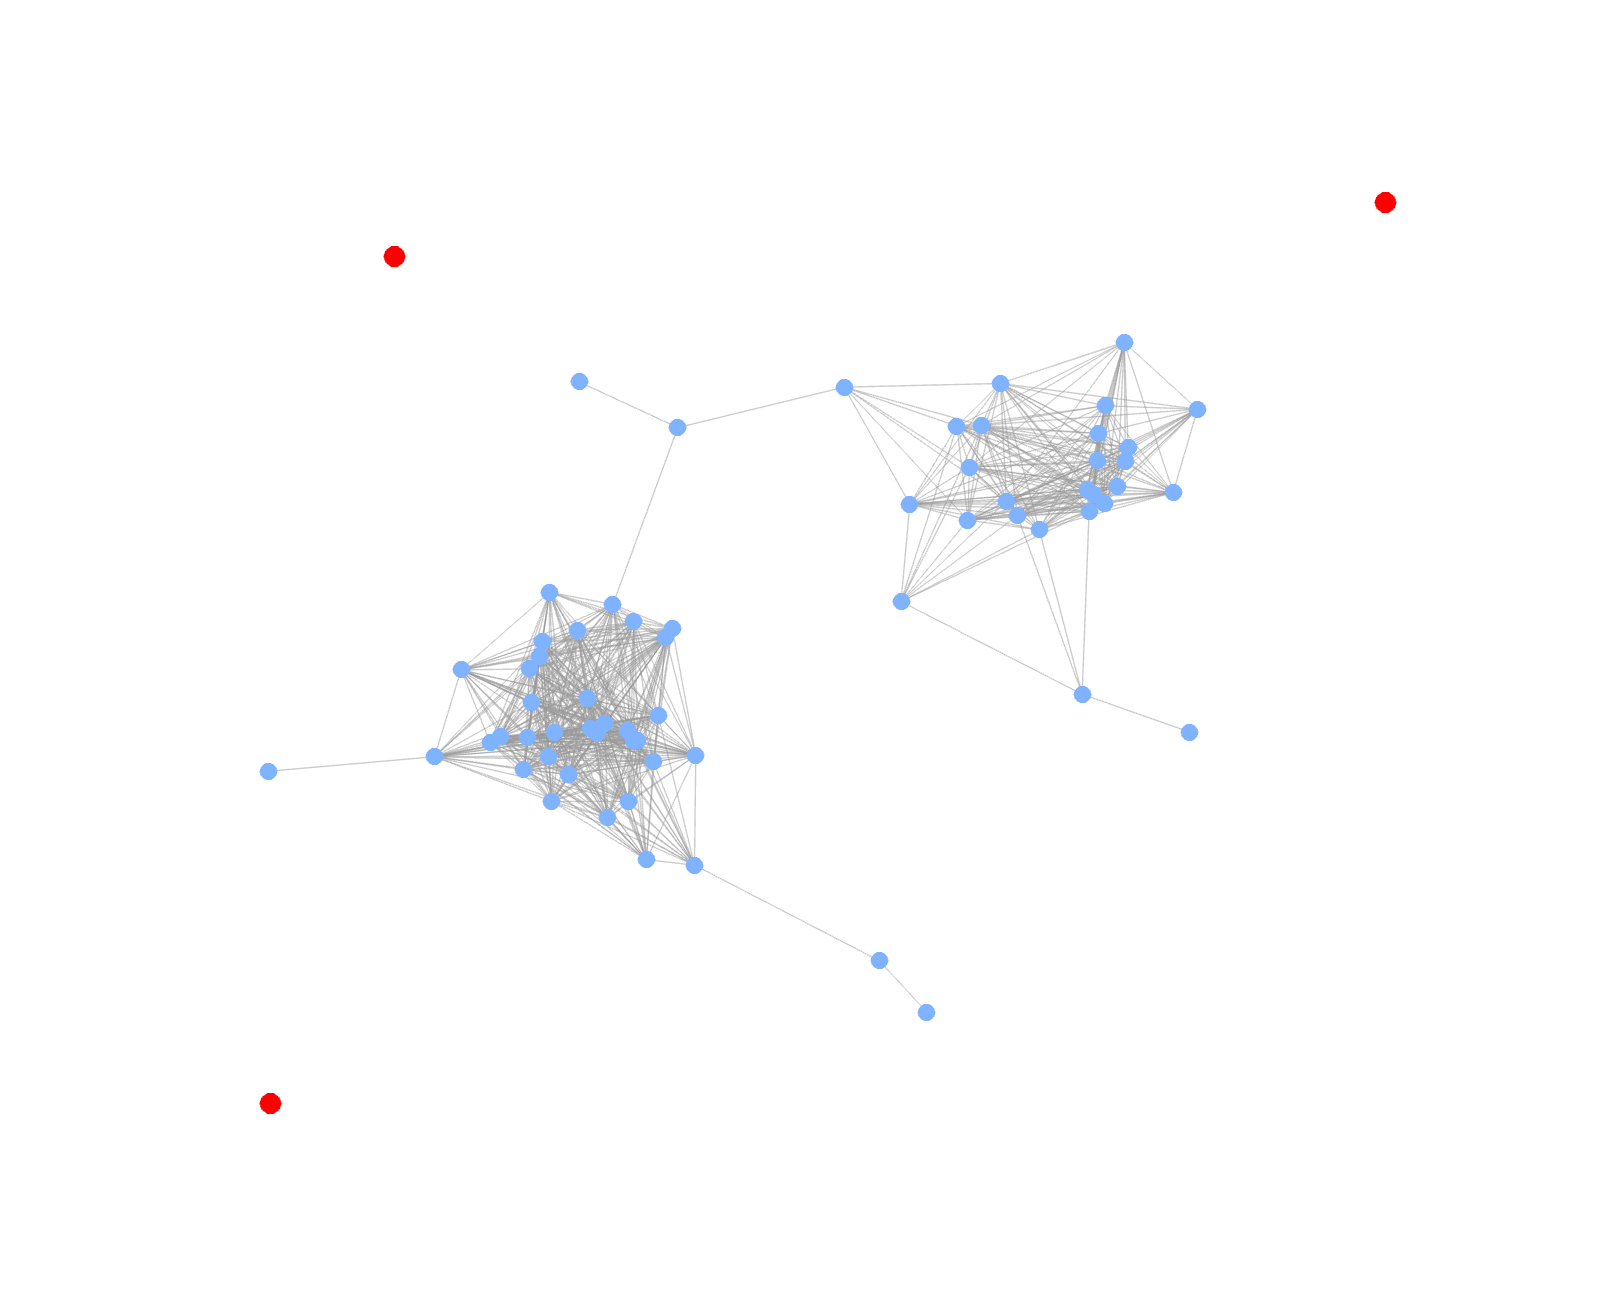
\includegraphics[width=0.9\textwidth]{img/robustness_problem.png}
        \caption{Illustration of the 'Isolated Student Locations' problem. Distant students (highlighted, e.g., in red) can necessitate disproportionately long and costly detours if included in standard routes, impacting overall efficiency.}
        \label{fig:problem_isolated_students}
    \end{figure}

    \item \textbf{Limited Service Capacity:} The university's bus fleet has specific capacity constraints. Each vehicle can typically accommodate a minimum of 10 and a maximum of 50 students. Clustering algorithms and route planning must strictly adhere to these capacity limits to ensure both operational feasibility and cost-effectiveness. Generating routes that are either too small (underutilized) or too large (exceeding capacity) is a key problem.

    \item \textbf{Fuel Consumption and Budget Limitations:} Fuel costs constitute a major portion of the transportation budget. Minimizing total distance traveled by all buses is a primary objective to reduce fuel consumption and operate within budgetary constraints. This necessitates the design of compact and efficient routes.

    \item \textbf{Large Number of Students:} With approximately 2000 students requiring transportation across a large metropolitan area, the scale of the network is substantial. This large number of nodes leads to high computational complexity for many graph algorithms, especially those involving dense matrix operations or exhaustive searches. Scalable and efficient algorithms are therefore essential.
    \begin{figure}[!htbp]
        \centering
        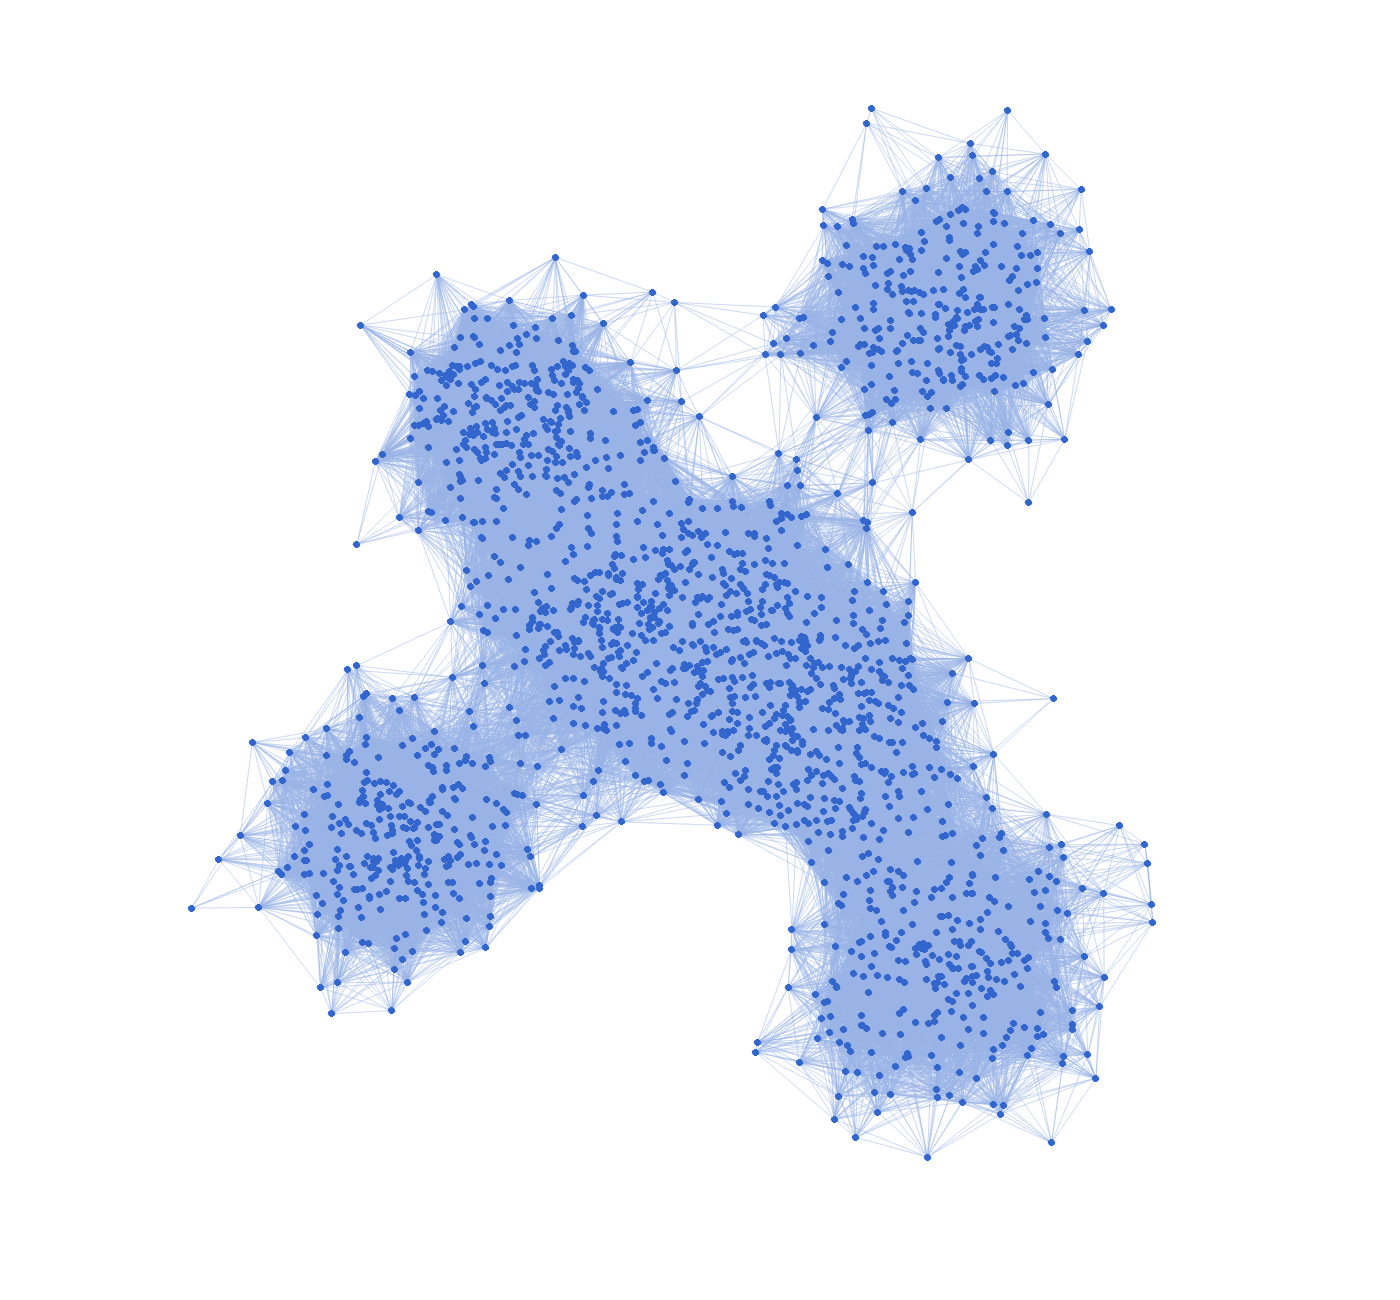
\includegraphics[width=0.7\textwidth]{img/large_scale_students.png}
        \caption{Representing the 'Large Number of Students' problem. The sheer volume and density of approximately 2000 student locations (nodes in the network), as illustrated here, significantly increase the computational complexity of finding optimal routing solutions.}
        \label{fig:problem_large_scale}
    \end{figure}

    \item \textbf{Non-Static Address Information:} While this thesis utilizes a synthetically generated dataset based on current general population distribution, in a real-world scenario, student address information can be non-static, changing semester by semester. An effective system should ideally be adaptable to such changes, although this aspect is more related to the operationalization than the core algorithmic design focused on here. The current work focuses on optimizing for a given snapshot of student locations.
\end{itemize}
Addressing these interconnected problems requires a holistic approach that balances cost, efficiency, service quality, and computational tractability.

\section{The Proposed Method}
\label{sec:intro_solution}
This thesis puts forth a solution focused on three primary contributions to optimize the IZTECH student transportation network, each addressing specific challenges outlined in Section~\ref{sec:intro_problems}:

\begin{enumerate}
    \item \textbf{Determining the necessary number of services and alternative solutions:} A key goal is to ascertain the optimal fleet size and explore various route configurations, thereby addressing the issues of Limited Service Capacity by ensuring routes adhere to the 10-50 student limit, and tackling the Large Number of Students by breaking the problem into manageable parts. Our approach achieves this by applying different graph clustering algorithms to partition the student population into potential bus routes, as detailed in Section~\ref{subsec:clustering_sparse}. By comparatively analyzing the outcomes—considering factors like the total number of routes, overall cost (which relates to Fuel Consumption and Budget Limitations), and adherence to capacity constraints—we identify a range of viable solutions and pinpoint the most efficient configurations \cite{zhang2018data}.
    
    \item \textbf{Efficiently determining service routes:} This refers to the development of computationally tractable and cost-effective methods for defining the actual paths for each bus service, directly targeting Fuel Consumption and Budget Limitations and the challenge of a Large Number of Students. We begin by employing sparse graph representations (specifically Delaunay Triangulation, Gabriel Graphs, and K-Nearest Neighbors Graphs) of the student network, as described in Section~\ref{subsec:sparse_graph}, which significantly reduces computational complexity. Once students are grouped via clustering, Dijkstra\'s algorithm (Section~\ref{sec:shortest_path}) is utilized to calculate the shortest path connecting students within each group, further minimizing travel distances and defining optimized service routes.
    
    \item \textbf{Ensuring robustness for isolated addresses:} This contribution directly tackles the problem of Isolated Student Locations, where students residing in geographically distant areas could lead to significant inefficiencies. Our solution incorporates a K-Nearest Neighbor (KNN) distance-based outlier detection method as a crucial preprocessing step (Section~\ref{subsec:knn_outlier_application}). This method identifies students whose locations are statistical outliers, allowing them to be handled separately or excluded. This not only improves route compactness, thereby contributing to reducing Fuel Consumption and Budget Limitations, thus enhancing the practicality and cost-effectiveness of the overall transportation plan.
\end{enumerate}

The comprehensive methodology to realize these contributions integrates these specific techniques. It begins with constructing an appropriate graph model of the student network using one of the selected sparse graph methods (Section~\ref{subsec:sparse_graph}). This is followed by the KNN distance-based outlier detection for data refinement (Section~\ref{subsec:knn_outlier_application}). Subsequently, a comparative evaluation of diverse graph clustering algorithms (Spectral Clustering, Leiden Algorithm, and Multi-view Anchor Graph-based Clustering), detailed in Section~\ref{subsec:clustering_sparse}, is performed to partition the students into capacity-constrained routes. Finally, Dijkstra's algorithm (Section~\ref{sec:shortest_path}) determines the optimal path for each route. The interplay between these components—graph construction, outlier detection, and clustering—is analyzed in detail to identify the most effective combination for the IZTECH student transportation problem.

\section{Thesis Overview}
\label{sec:intro_overview}
This thesis is structured to systematically present the research methodology, experimental evaluation, and findings.
\begin{itemize}
    \item \textbf{Chapter~\ref{ch:introduction}} (this chapter) outlines the motivation, discusses the state-of-the-art, defines the problem scope, introduces our proposed solution, and provides this overview of the thesis structure.
    \item \textbf{Chapter~\ref{ch:basics}} provides the necessary theoretical background. It covers fundamental concepts in graph theory, details various graph construction methods and the significance of sparsity, explains the principles behind the selected graph clustering algorithms (Spectral Clustering, Leiden Algorithm, MVAGC), discusses shortest path computation (Dijkstra's algorithm), and introduces the K-Nearest Neighbor distance-based outlier detection technique.
    \item \textbf{Chapter~\ref{ch:method}} details the specific methodologies employed in this research. This includes the generation of the synthetic student dataset, the practical implementation of the different graph construction techniques (Complete, Delaunay, Gabriel, KNN), the adaptation and application of the clustering algorithms to these graphs with capacity constraints, the implementation of the outlier detection process, and the method for shortest path calculation within clusters.
    \item \textbf{Chapter~\ref{ch:experiments}} presents a comprehensive experimental evaluation of the proposed methods. It compares the performance of different combinations of graph construction techniques and clustering algorithms, both with and without outlier detection. The evaluation is based on key metrics including total transportation cost, number of routes, average route length, average cluster size, and computational time. The results are analyzed to identify the most effective and efficient approaches.
    \item \textbf{Chapter~\ref{ch:conclusions}} summarizes the key findings of the research, discusses the main contributions of the thesis to the field of transportation network optimization, and suggests potential avenues for future work, including methodological advancements and practical implementations.
    \item The \textbf{Appendix} may contain supplementary materials, such as detailed experimental results or pseudocode for algorithms not fully detailed in the main text.
\end{itemize}
Through this structured approach, the thesis aims to provide a clear and thorough investigation into optimizing university student transportation networks using graph-based methods.




l
\chapter{Theoretical Background}
\label{ch:basics}
This chapter introduces the fundamental concepts and theories used in transportation network analysis. First, we explore basic graph theory concepts essential for understanding networks. Then, we examine how transportation systems can be represented as graphs. Finally, we discuss clustering algorithms applied to identify communities within these networks, with focus on their applications in transportation systems .

\section{Basic Definitions}
\label{se:BasicDefinitions}

A graph $G$ is formally defined as an ordered pair $G = (V, E, W)$ comprising a set $V$ of vertices or nodes and a set $E$ of edges, which are 2-element subsets of $V$ . The fundamental components of a graph include: \textbf{Vertices (Nodes)} which represent distinct entities in the network; \textbf{Edges} which represent the connections or relationships between vertices; \textbf{Affinity Matrix} $W$, which is a square matrix where each element $W_{ij}$ represents the weight between vertices $i$ and $j$, indicating distances, travel times, costs, or other metrics.


\section{Graph Construction Methods and Sparsity}
\label{se:GraphConstructionMethodsAndSparsity}

Graph construction methods determine how nodes in a network are connected, playing a crucial role in creating accurate transportation network representations by balancing connectivity with computational efficiency.

A graph is considered complete if every distinct pair of vertices is connected by an edge. In terms of edge weights \(w_{i,j}\), this means a connection exists for all \(i \neq j\). While this represents the maximum possible connectivity, constructing a complete graph for a transportation network is often impractical. It implies direct travel is possible between any two locations, ignoring real-world constraints like geographical barriers or infrastructure costs. Such dense connectivity is computationally expensive to analyze and does not accurately reflect most transportation systems. Therefore, sparsity, where only essential or feasible connections are represented, becomes crucial for creating realistic and manageable network models.

\subsubsection{K-Nearest Neighbors Graph}
In this approach, each vertex is connected to its $k$ nearest neighbors according to some distance metric . This method creates a sparse graph where each location is connected only to its closest locations.

\begin{equation}
    E = \{(u, v) \mid v \in \text{kNN}(u) \text{ or } u \in \text{kNN}(v)\}
\end{equation}
where $\text{kNN}(u)$ represents the $k$ nearest neighbors of vertex $u$.

\subsubsection{Delaunay Triangulation}
Delaunay triangulation creates a graph by connecting vertices such that no vertex lies inside the circumcircle of any triangle formed by three connected vertices . This method preserves local connectivity while avoiding crossing edges, making it useful for geographic applications.

\subsubsection{Gabriel Graph}
The Gabriel Graph is a subgraph of the Delaunay triangulation . An edge connects two vertices $u$ and $v$ if and only if the circle with diameter $uv$ contains no other vertices.

\begin{equation}
    E = \{(u, v) \mid d^2(u, v) < d^2(u, w) + d^2(v, w) \text{ for all } w \in V, w \neq u, w \neq v\}
\end{equation}
where $d(u, v)$ is the distance between vertices $u$ and $v$.

\section{Graph-based Clustering}
\label{se:GraphBasedClusterings}

Clustering in graphs involves partitioning the vertices into cohesive groups or communities based on connectivity patterns, proximity, or other relevant factors. These clusters can represent meaningful subgroups or structures within the data represented by the graph.

\subsection{Spectral Clustering}
\label{subsec:SpectralClustering}

Spectral clustering uses the eigenvalues and eigenvectors of matrices derived from the graph to perform dimensionality reduction before clustering . This approach is particularly effective for finding natural clusters in complex networks. The algorithm is summarized in Algorithm~\ref{alg:spectral_clustering}.

\begin{algorithm}[H]
\caption{Spectral Clustering}
\label{alg:spectral_clustering}
\begin{algorithmic}[1]
\Require Graph $G = (V, E)$, number of clusters $k$
\Ensure Cluster assignments for vertices $V$

\State Construct the Adjacency Matrix $\mat{A}$ for the graph $G$.
\State Construct the Edge Weight Matrix $\mat{D}$ where $\mat{d}_{ii} = \sum_j \mat{A}_{ij}$.
\State Calculate the Laplacian Matrix $\mat{L} = \mat{D} - \mat{A}$.
\State Compute the Normalized Laplacian $\mat{L}_{\text{norm}} = \mat{D}^{-1/2} \mat{L} \mat{D}^{-1/2} = \mat{I} - \mat{D}^{-1/2} \mat{A} \mat{D}^{-1/2}$.
\State Find the $k$ eigenvectors $\vect{u}_1, \vect{u}_2, \dots, \vect{u}_k$ corresponding to the $k$ smallest non-zero eigenvalues of $\mat{L}_{\text{norm}}$.
\State Form the matrix $U \in \R^{|V| \times k}$ with the eigenvectors $\vect{u}_1, \dots, \vect{u}_k$ as columns.
\State Let $\vect{y}_i \in \R^k$ be the vector corresponding to the $i$-th row of $U$.
\State Cluster the points $(\vect{y}_i)_{i=1, \dots, |V|}$ into $k$ clusters $C_1, \dots, C_k$ using the $k$-means algorithm.
\State Assign vertex $v_i$ to cluster $C_j$ if row $\vect{y}_i$ was assigned to cluster $C_j$.

\end{algorithmic}
\end{algorithm}


\subsection{Leiden Algorithm}
\label{subsec:LeidenAlgorithm}

The Leiden algorithm improves upon the Louvain algorithm for community detection by ensuring well-connected communities and optimizing modularity. The algorithm operates iteratively to detect communities within a graph. Starting with each node in its own community (a singleton partition), the algorithm performs a local moving phase where individual nodes are reassigned to neighboring communities if such a move improves the overall modularity. This phase continues until no single node move can further increase modularity, resulting in an initial partition. Subsequently, a refinement phase ensures that the communities formed are well-connected by partitioning each community internally. An aggregate network is then constructed based on this refined partition, where each node represents a subcommunity from the refinement stage. The non-refined partition from the local moving phase serves as the initial community assignment for this aggregate network. For instance, if a community is split into two subcommunities during refinement, these become two distinct nodes in the aggregate network, initially assigned to the same aggregate community. The algorithm then repeats the local moving and refinement phases on the aggregate network. These steps of local moving, refinement, and aggregation are iterated until no further improvements in modularity can be achieved, yielding the final community structure. The detailed pseudocode can be found in Appendix \ref{alg:leiden_appendix}.

The key innovations of the Leiden algorithm over its predecessors include faster convergence due to more efficient community detection, guaranteed well-connected communities through the refinement phase, the ability to avoid getting trapped in poor local optima by allowing more flexible node movement, and proven asymptotic guarantees for identifying optimal partitions \cite{traag2019leiden}.


\subsection{Multi-view Anchor Graph-based Clustering (MVAGC)}
\label{subsec:MVAGC}

Multi-view Anchor Graph-based Clustering (MVAGC) is an advanced clustering technique designed to handle complex datasets represented by multiple feature sets or 'views'. 

The core idea of MVAGC is to leverage the complementary information present in these different views to obtain a more robust and meaningful clustering result than using any single view alone. Instead of working with the potentially very large full graph, MVAGC utilizes a smaller set of 'anchor points'. These anchors are selected representative points from the dataset (either strategically chosen or randomly sampled).

\begin{algorithm}[H]
\caption{Multi-view Anchor Graph-based Clustering (MVAGC)}
\label{alg:mvagc}
\begin{algorithmic}[1]
\Require Data points $V = \{v_1, \dots, v_n\}$, Multiple view data representations $X^{(1)}, \dots, X^{(p)}$, Number of clusters $k$, Number of anchors $m$
\Ensure Cluster assignments for vertices $V$

\State Select $m$ anchor points $U = \{u_1, \dots, u_m\}$ from $V$ (e.g., using k-means or random sampling).
\For{each view $v = 1, \dots, p$}
    \State Construct view-specific anchor relationship matrix $Z^{(v)} \in \R^{n \times m}$. $Z_{ij}^{(v)}$ represents the similarity/connection between data point $v_i$ and anchor $u_j$ in view $v$.
\EndFor
\State Fuse the view-specific matrices $\{Z^{(1)}, \dots, Z^{(p)}\}$ into a unified representation. This often involves solving an optimization problem to find a consensus matrix $Z^*$ or graph structure that integrates information across views. 
    \Comment{E.g., Minimize $\sum_{v=1}^{p} \| Z^{(v)} - \text{f}(Z^*, \dots) \|_F^2 + \lambda \cdot \text{Regularization}(Z^*)$}
\State Perform clustering based on the fused representation $Z^*$.
    \If{$Z^*$ represents point-to-anchor assignments}
        \State Apply k-means or spectral clustering on the rows of $Z^*$ (representing points in the anchor space).
    \ElsIf{$Z^*$ is used to derive a consensus anchor graph $A_{\text{anchor}} \in \R^{m \times m}$}
        \State Apply spectral clustering on $A_{\text{anchor}}$ to cluster the anchors.
        \State Assign original points $v_i$ to the cluster of their nearest anchor based on $Z^*$.
    \EndIf
\State Assign final cluster labels $C_1, \dots, C_k$ to the original data points $V$.

\end{algorithmic}
\end{algorithm}

\section{Shortest Path Algorithms}
\label{se:ShortestPathAlgorithms}

Shortest path algorithms are fundamental for transportation network analysis, allowing us to determine the most efficient route between locations. In our work, we focused primarily on Dijkstra's algorithm due to its efficiency and suitability for transportation networks with non-negative edge weights.

\subsection{Dijkstra's Algorithm}
\label{subsec:DijkstrasAlgorithm}

Dijkstra's algorithm solves the single-source shortest path problem for a weighted graph with non-negative edge weights. Given a weighted graph $G = (V, E)$ with vertices $V$ and edges $E$, and a source vertex $s \in V$, Dijkstra's algorithm finds the shortest path from $s$ to every other vertex in the graph.

For a weighted graph $G = (V, E)$ with a weight function $w: E \rightarrow \mathbb{R}^+$ (assigning non-negative weights to edges), Dijkstra's algorithm maintains two primary values for each vertex $v \in V$: First, $\text{dist}[v]$ represents the currently known shortest distance from source $s$ to vertex $v$; Second, $\text{prev}[v]$ indicates the predecessor of $v$ in the shortest path from $s$ to $v$.

The algorithm initializes $\text{dist}[s] = 0$ and $\text{dist}[v] = \infty$ for all other vertices $v \in V \setminus \{s\}$. The iterative process then begins by selecting the unvisited vertex $u$ with the smallest distance value $\text{dist}[u]$. After marking $u$ as visited, the algorithm updates the distance values of all neighboring vertices $v$ according to the following formula:

\begin{equation}
\text{dist}[v] = \min(\text{dist}[v], \text{dist}[u] + w(u, v))
\end{equation}

where $w(u, v)$ is the weight of the edge from $u$ to $v$.

When a shorter path is discovered and the distance is updated, the predecessor is also updated:

\begin{equation}
\text{prev}[v] = u
\end{equation}

\begin{algorithm}[H]
\caption{Dijkstra's Shortest Path Algorithm}
\label{alg:dijkstra}
\begin{algorithmic}[1]
\Require Graph $G = (V, E)$, Source vertex $s \in V$, Weight function $w: E \rightarrow \mathbb{R}^+$
\Ensure Shortest path from $s$ to all vertices in $V$

\State Initialize $\text{dist}[s] \gets 0$ and $\text{dist}[v] \gets \infty$ for all $v \in V \setminus \{s\}$
\State Initialize $\text{prev}[v] \gets \text{null}$ for all $v \in V$
\State Initialize set of unvisited vertices $Q \gets V$

\While{$Q \neq \emptyset$}
    \State $u \gets \text{vertex in } Q \text{ with min } \text{dist}[u]$ \Comment{Extract min operation}
    \State Remove $u$ from $Q$
    
    \For{each neighbor $v$ of $u$ in $G$}
        \State $\text{alt} \gets \text{dist}[u] + w(u, v)$ \Comment{Distance through $u$ to $v$}
        \If{$\text{alt} < \text{dist}[v]$}
            \State $\text{dist}[v] \gets \text{alt}$ \Comment{Update distance}
            \State $\text{prev}[v] \gets u$ \Comment{Update predecessor}
        \EndIf
    \EndFor
\EndWhile

\State \Return $\text{dist}$ and $\text{prev}$ arrays
\end{algorithmic}
\end{algorithm}

\chapter{Methodology}
\label{ch:method}

This chapter details the methodology employed to analyze and optimize the transportation network for students of the Izmir Institute of Technology residing in Izmir. The primary objective is to identify efficient bus routing strategies that minimize overall fuel consumption while adhering to practical constraints on bus capacity. Specifically, the network serves approximately 2000 students, and routes must accommodate a minimum of 10 and a maximum of 50 students per vehicle. 

Our approach leverages graph theory, treating student locations as nodes and potential travel segments as edges. We systematically explore various graph construction techniques and clustering algorithms to model the spatial relationships and identify optimal bus routes. The methodology is divided into three main sections: graph representation of the transportation map, clustering of the graph representations, and robustness analysis for the clustering solutions.

\section{Graph Representation of Transportation Map of IZTECH}
\label{sec:graph_representation}

The foundation of our analysis is a dataset comprising the geographical coordinates of approximately 2000 synthetically generated student locations throughout Izmir. These points were created by applying a Gaussian distribution based on the actual population data for each district in Izmir. Figure \ref{fig:student_map} illustrates the geographical distribution of these student locations. In our graph-based model, each student's location is represented as a distinct node (or vertex) $v$ within a set $V$. The set $V$ thus encapsulates all student locations considered in the transportation network, where $|V| \approx 2000$. 

% Placeholder for Map Visualization
\begin{figure}[!htbp]
\centering
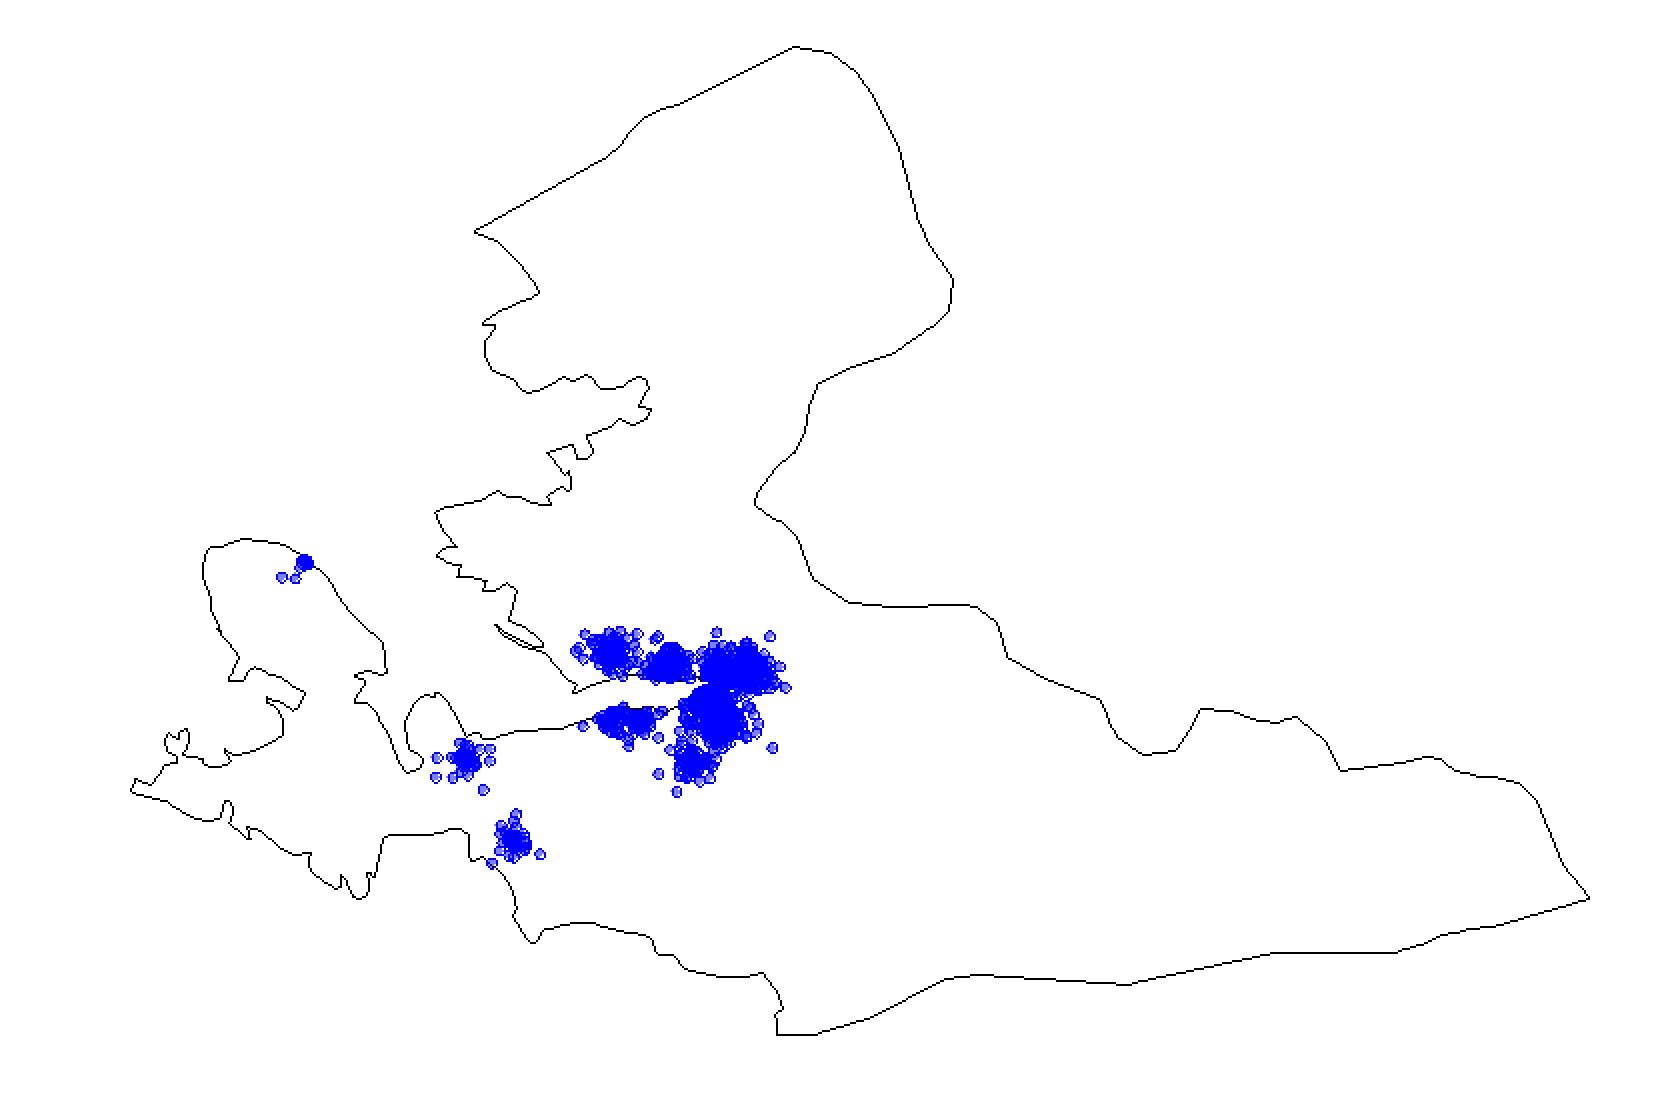
\includegraphics[width=0.8\textwidth]{img/student_map}
\caption{Geographical distribution of student locations in Izmir.}
\label{fig:student_map}
\end{figure}

\subsection{Complete Graph of Transportation Map}
\label{subsec:complete_graph}

A complete graph is the natural mathematical representation of a transportation network where every location is directly connected to every other location. Formally, for our set of student locations $V$, the complete graph $G_{complete} = (V, E_{complete})$ contains an edge $e_{uv} \in E_{complete}$ for every pair of distinct vertices $u, v \in V$, resulting in $|E_{complete}| = {|V| \choose 2} = \frac{|V|(|V|-1)}{2}$ edges. The complete graph connects every pair of distinct student locations, representing maximum potential connectivity as detailed in Section~\ref{se:GraphConstructionMethodsAndSparsity}.

This representation serves as our baseline model, establishing upper bounds on connectivity. However, the dense connectivity often leads to suboptimal routing solutions with higher overall costs due to the ${|V| \choose 2}$ edges making it computationally expensive for large datasets.

\begin{figure}[!htbp]
\centering
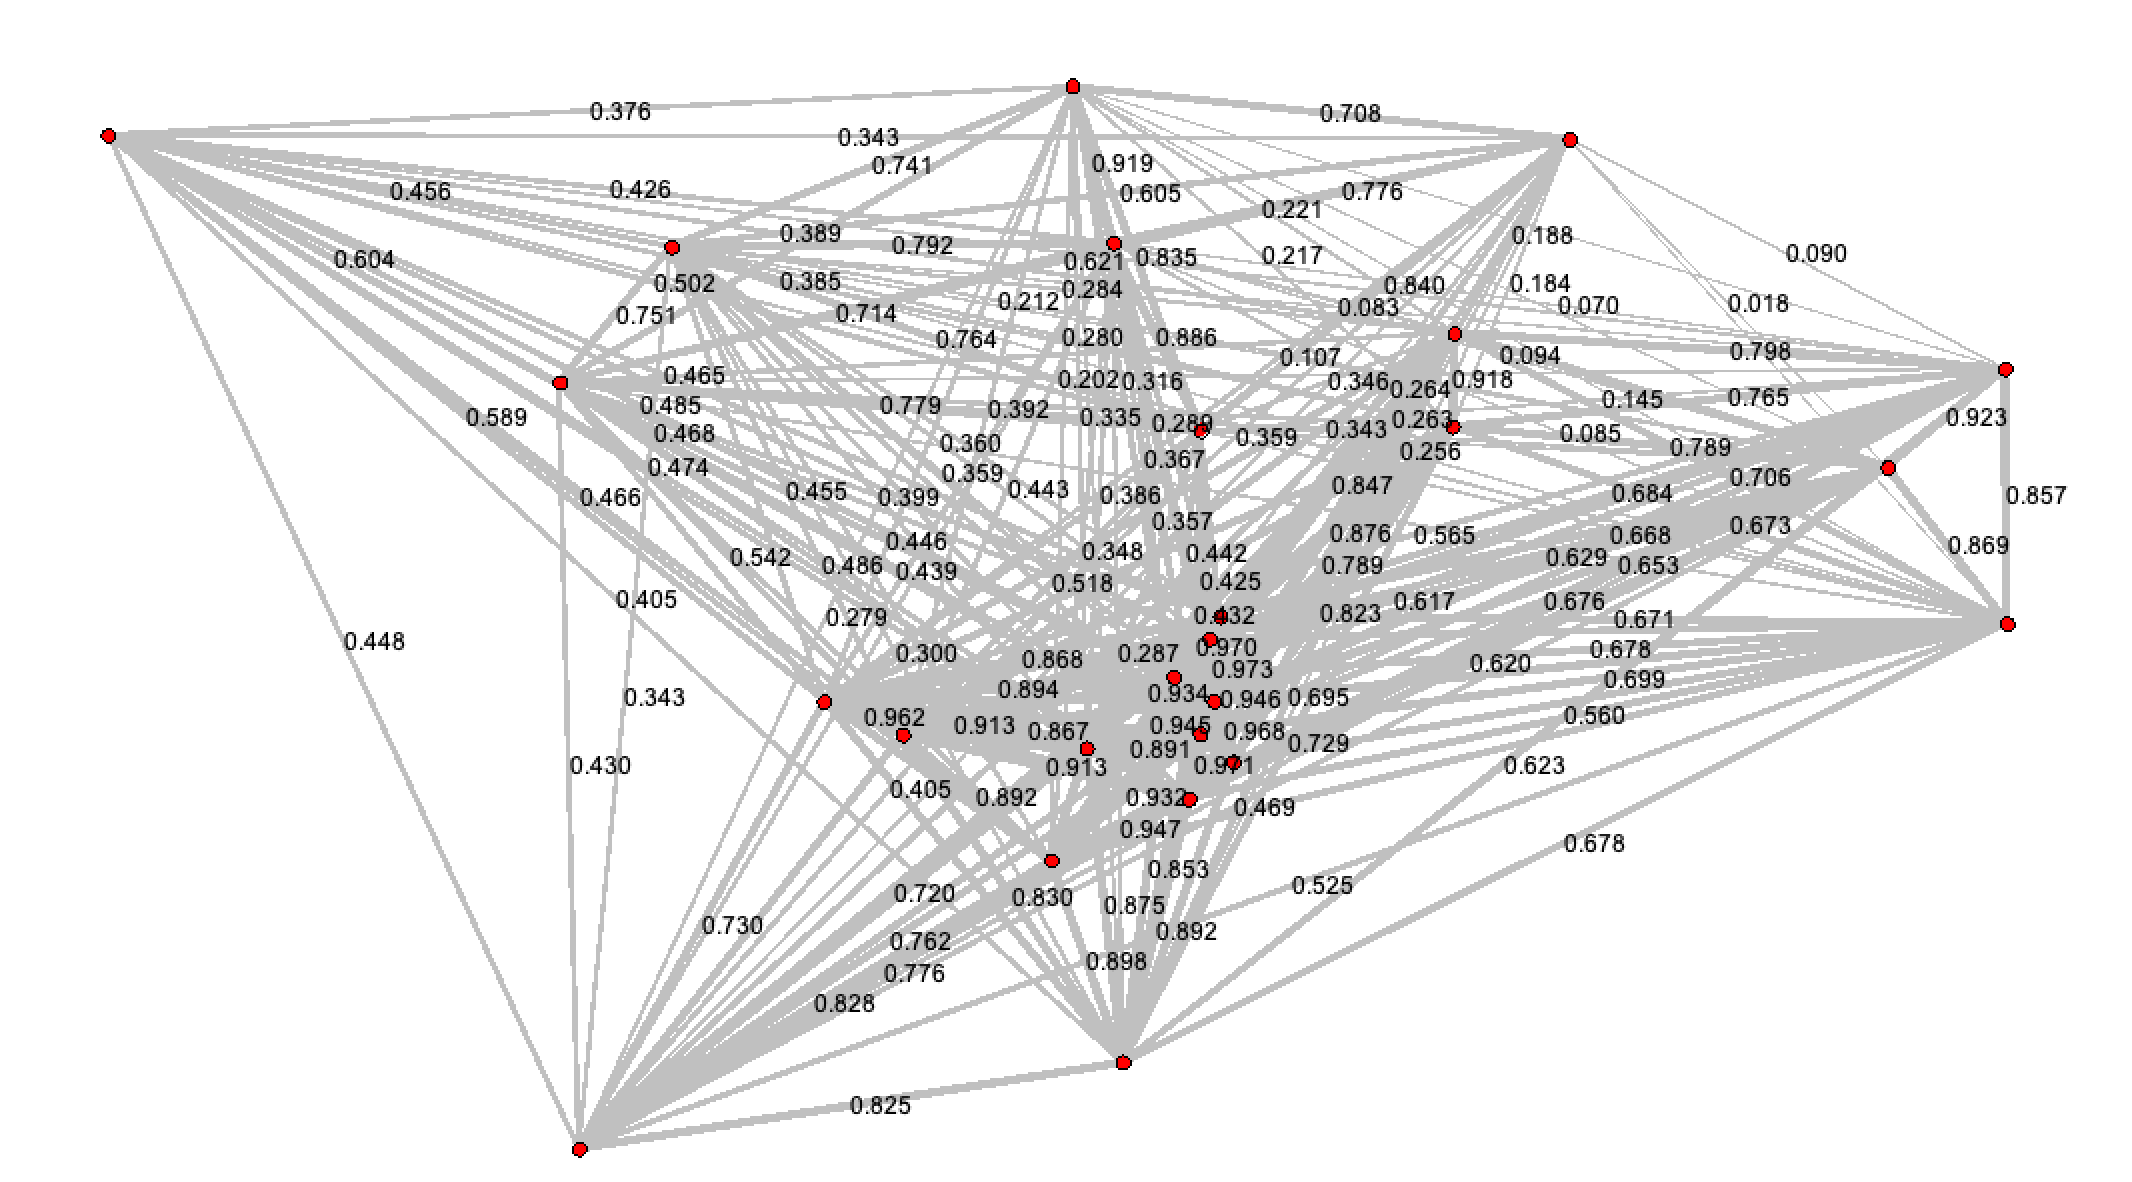
\includegraphics[width=0.6\textwidth]{img/complete}
\caption{Complete graph representation of a sample of student locations. Every point is connected to every other point, representing maximum connectivity but leading to computational challenges for large datasets.}
\label{fig:complete_graph}
\end{figure}



\subsection{Sparse Graph Representation}
\label{subsec:sparse_graph}

Given the computational and practical limitations of the complete graph approach, we explored several sparse graph construction techniques that preserve essential connectivity while significantly reducing the number of edges. These methods emphasize local connections and spatial proximity, resulting in more efficient representations of the transportation network.

\subsubsection{Delaunay Graph Representation}
\label{subsubsec:delaunay}

The Delaunay triangulation constructs a graph $G_{Delaunay}=(V, E_{Delaunay})$ based on the empty circumcircle property as explained in Section~\ref{se:GraphConstructionMethodsAndSparsity}. For any three vertices $p, q, r \in V$, they form a triangle in the Delaunay triangulation if and only if the circumcircle passing through $p, q, r$ contains no other vertex in $V$. This property creates a planar graph that avoids edge crossings and naturally connects proximate points.

\begin{figure}[!htbp]
\centering
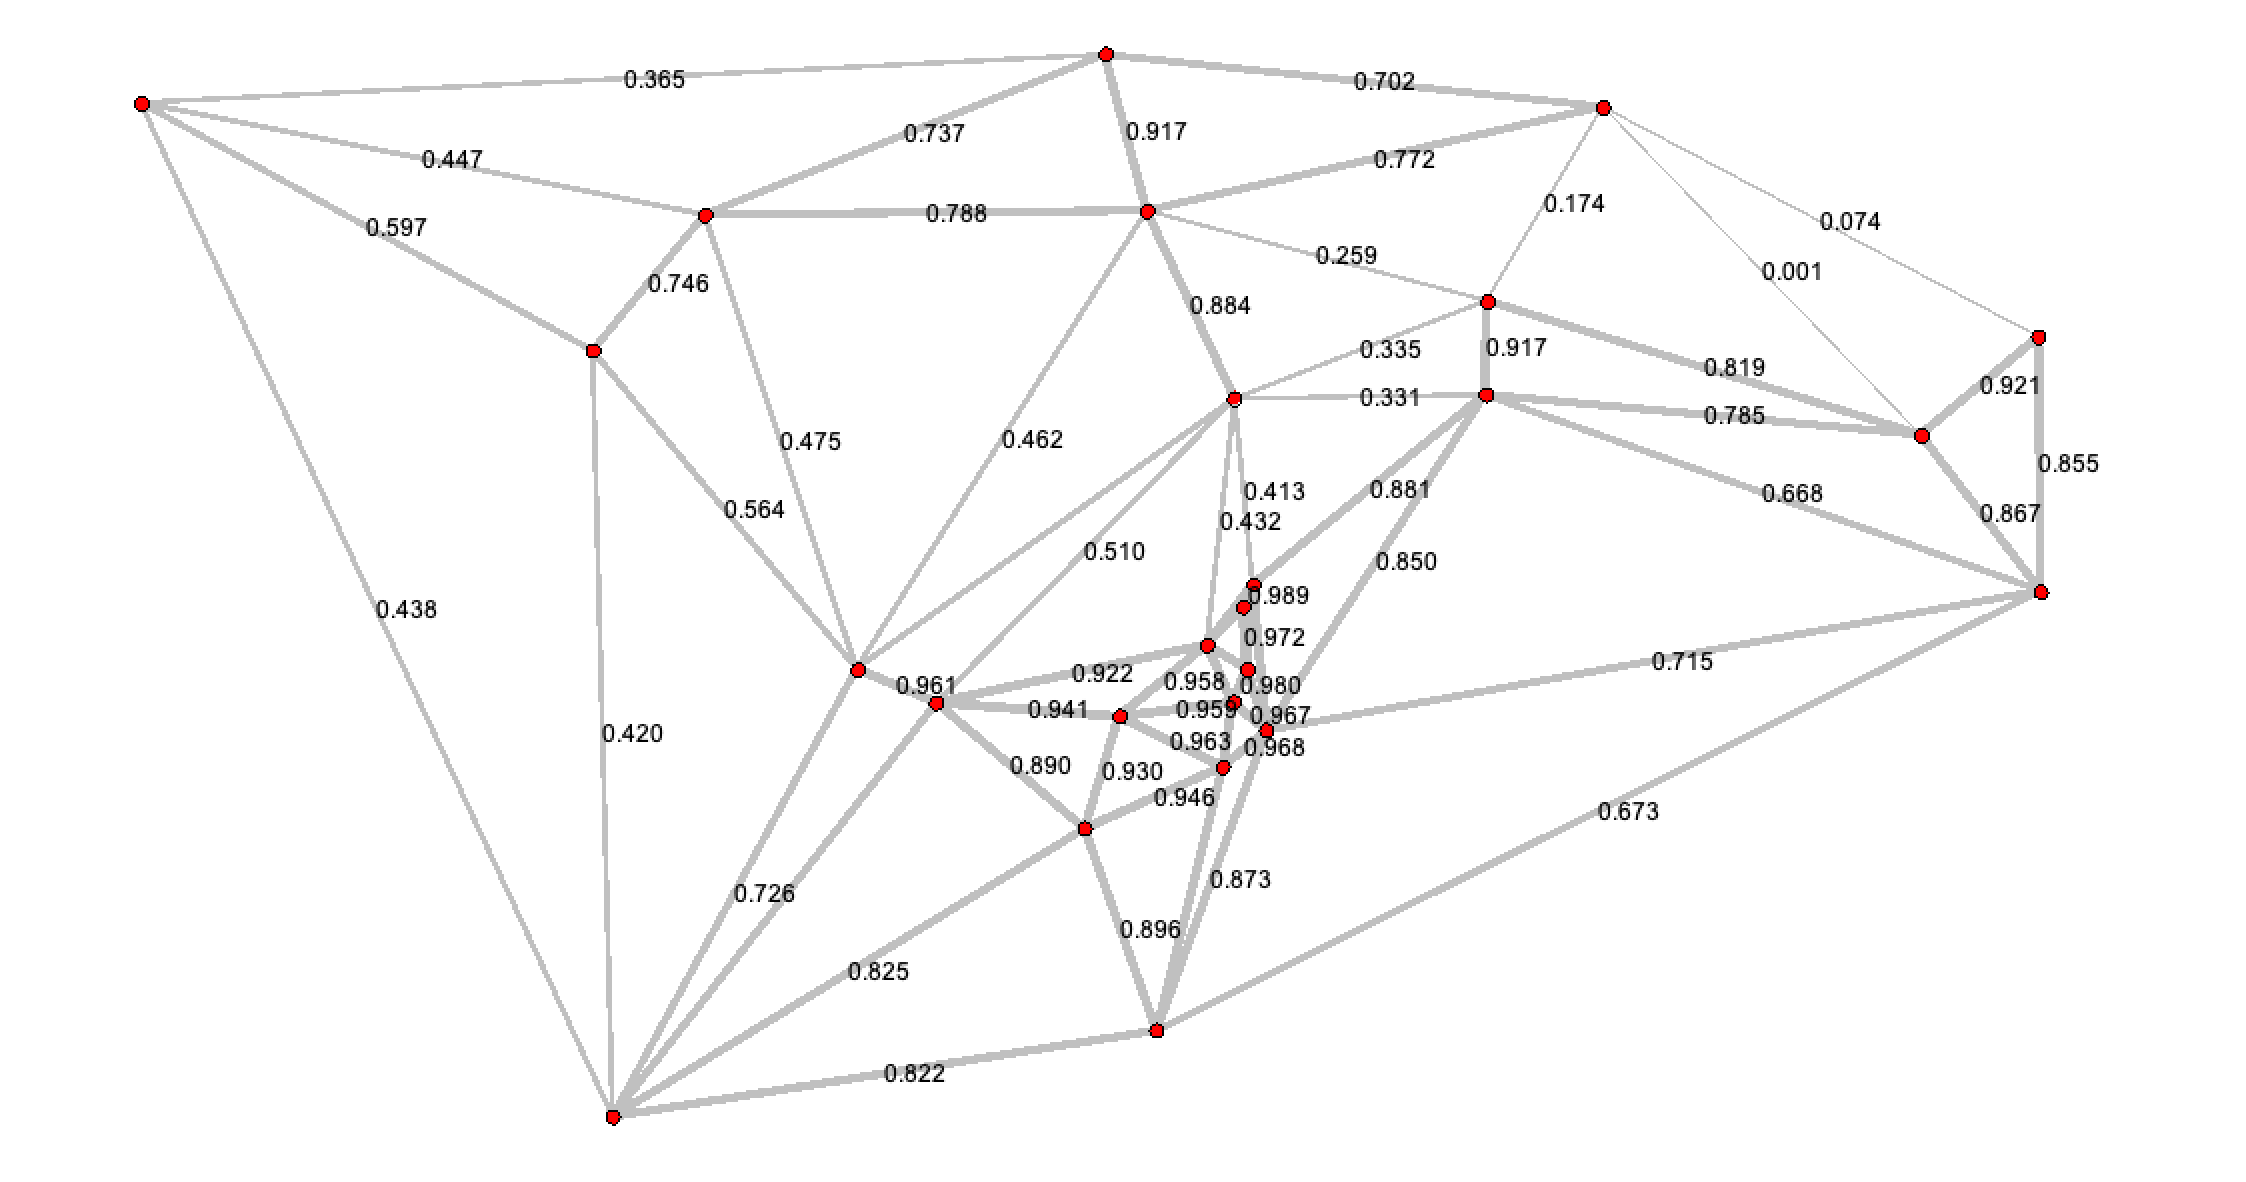
\includegraphics[width=0.6\textwidth]{img/delaunay}
\caption{Delaunay triangulation applied to a sample of student locations. The triangulation connects points such that no point lies inside the circumcircle of any triangle, creating a network that naturally preserves proximity relationships.}
\label{fig:delaunay_graph}
\end{figure}

\subsubsection{Gabriel Graph Representation}
\label{subsubsec:gabriel}

The Gabriel graph is a subgraph of the Delaunay triangulation that connects nodes if the circle with diameter between them contains no other nodes (see Section~\ref{se:GraphConstructionMethodsAndSparsity}). Formally, for our set of student locations $V$, the Gabriel graph $G_{Gabriel}=(V, E_{Gabriel})$ contains an edge $e_{uv} \in E_{Gabriel}$ if and only if:

\begin{equation}
d^2(u, v) < d^2(u, w) + d^2(v, w) \text{ for all } w \in V, w \neq u, w \neq v
\end{equation}

where $d(u, v)$ represents the Euclidean distance between vertices $u$ and $v$.

Our implementation constructs the Gabriel graph by first generating the Delaunay triangulation and then filtering edges based on the empty circle criterion. This approach preserves the most efficient local connections while further reducing the computational complexity compared to the complete graph.

\begin{figure}[!htbp]
\centering
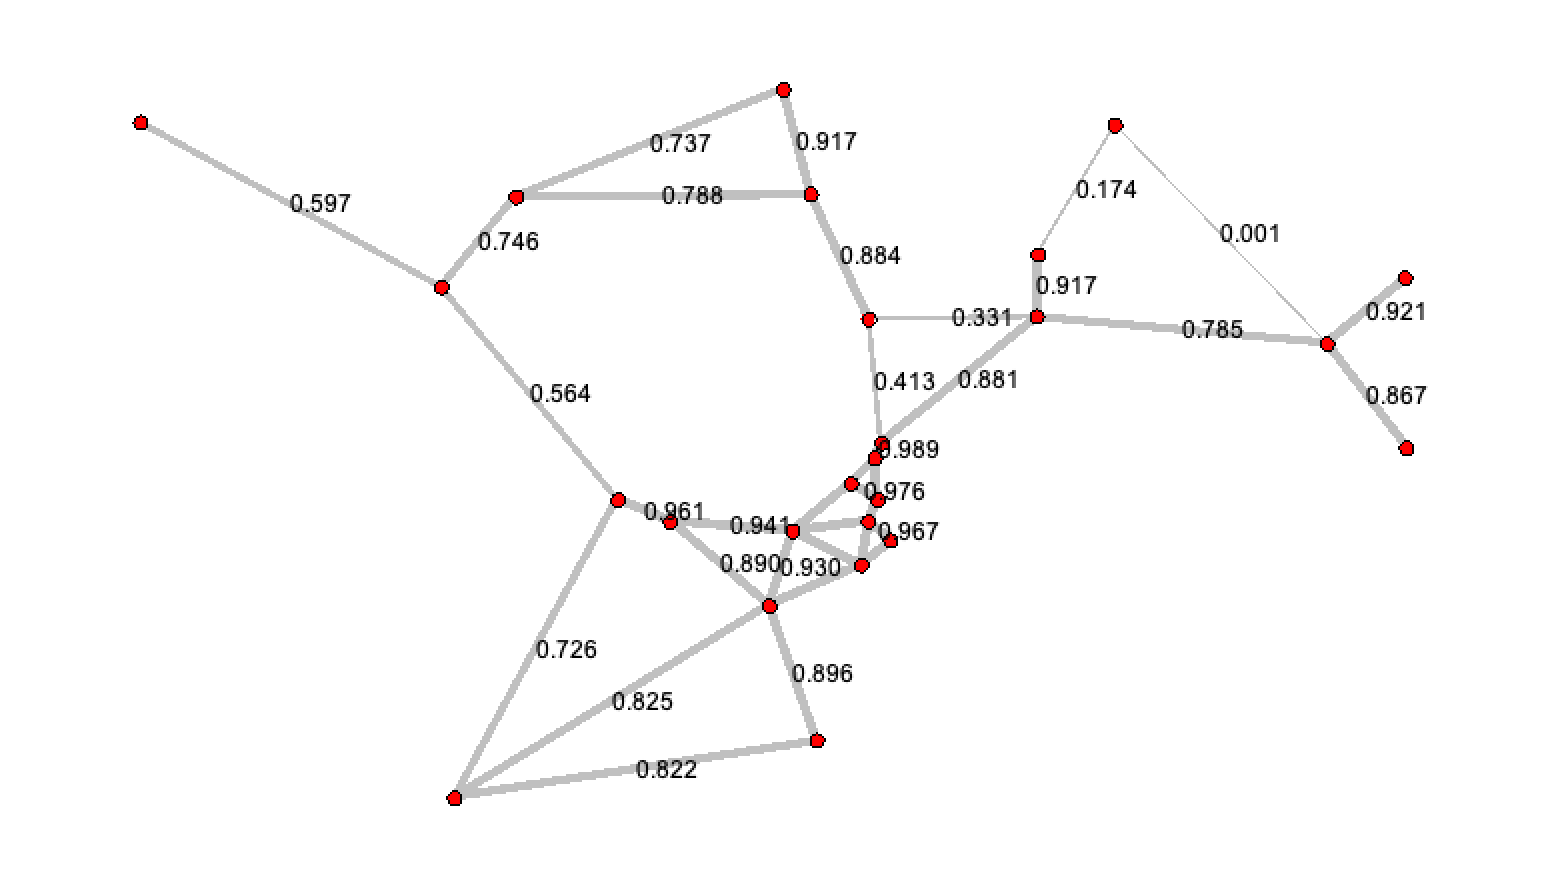
\includegraphics[width=0.6\textwidth]{img/gabriel}
\caption{Gabriel graph derived from student location data. This graph is a subgraph of the Delaunay triangulation, where an edge between two points exists only if the circle with the diameter equal to the distance between them contains no other points.}
\label{fig:gabriel_graph}
\end{figure}

\subsubsection{K-Nearest Neighbour Graph Representation}
\label{subsubsec:knn}

The K-Nearest Neighbors (KNN) graph connects each node to its $k$ closest neighbors, creating a sparse representation that emphasizes local connectivity as detailed in Section~\ref{se:GraphConstructionMethodsAndSparsity}. For our set of student locations $V$, the KNN graph $G_{KNN}=(V, E_{KNN})$ contains edges such that:

\begin{equation}
E_{KNN} = \{(u, v) \mid v \in \text{kNN}(u) \text{ or } u \in \text{kNN}(v)\}
\end{equation}

where $\text{kNN}(u)$ represents the $k$ nearest neighbors of vertex $u$ according to Euclidean distance.

In our implementation, we set $k=30$ based on the average seat size of buses in the IZTECH fleet, ensuring that each node is connected to approximately the number of students that would typically share transportation. The graph is constructed using spatial indexing for efficient neighbor queries, with edge weights based on the Euclidean distance between connected nodes.

\begin{figure}[!htbp]
\centering
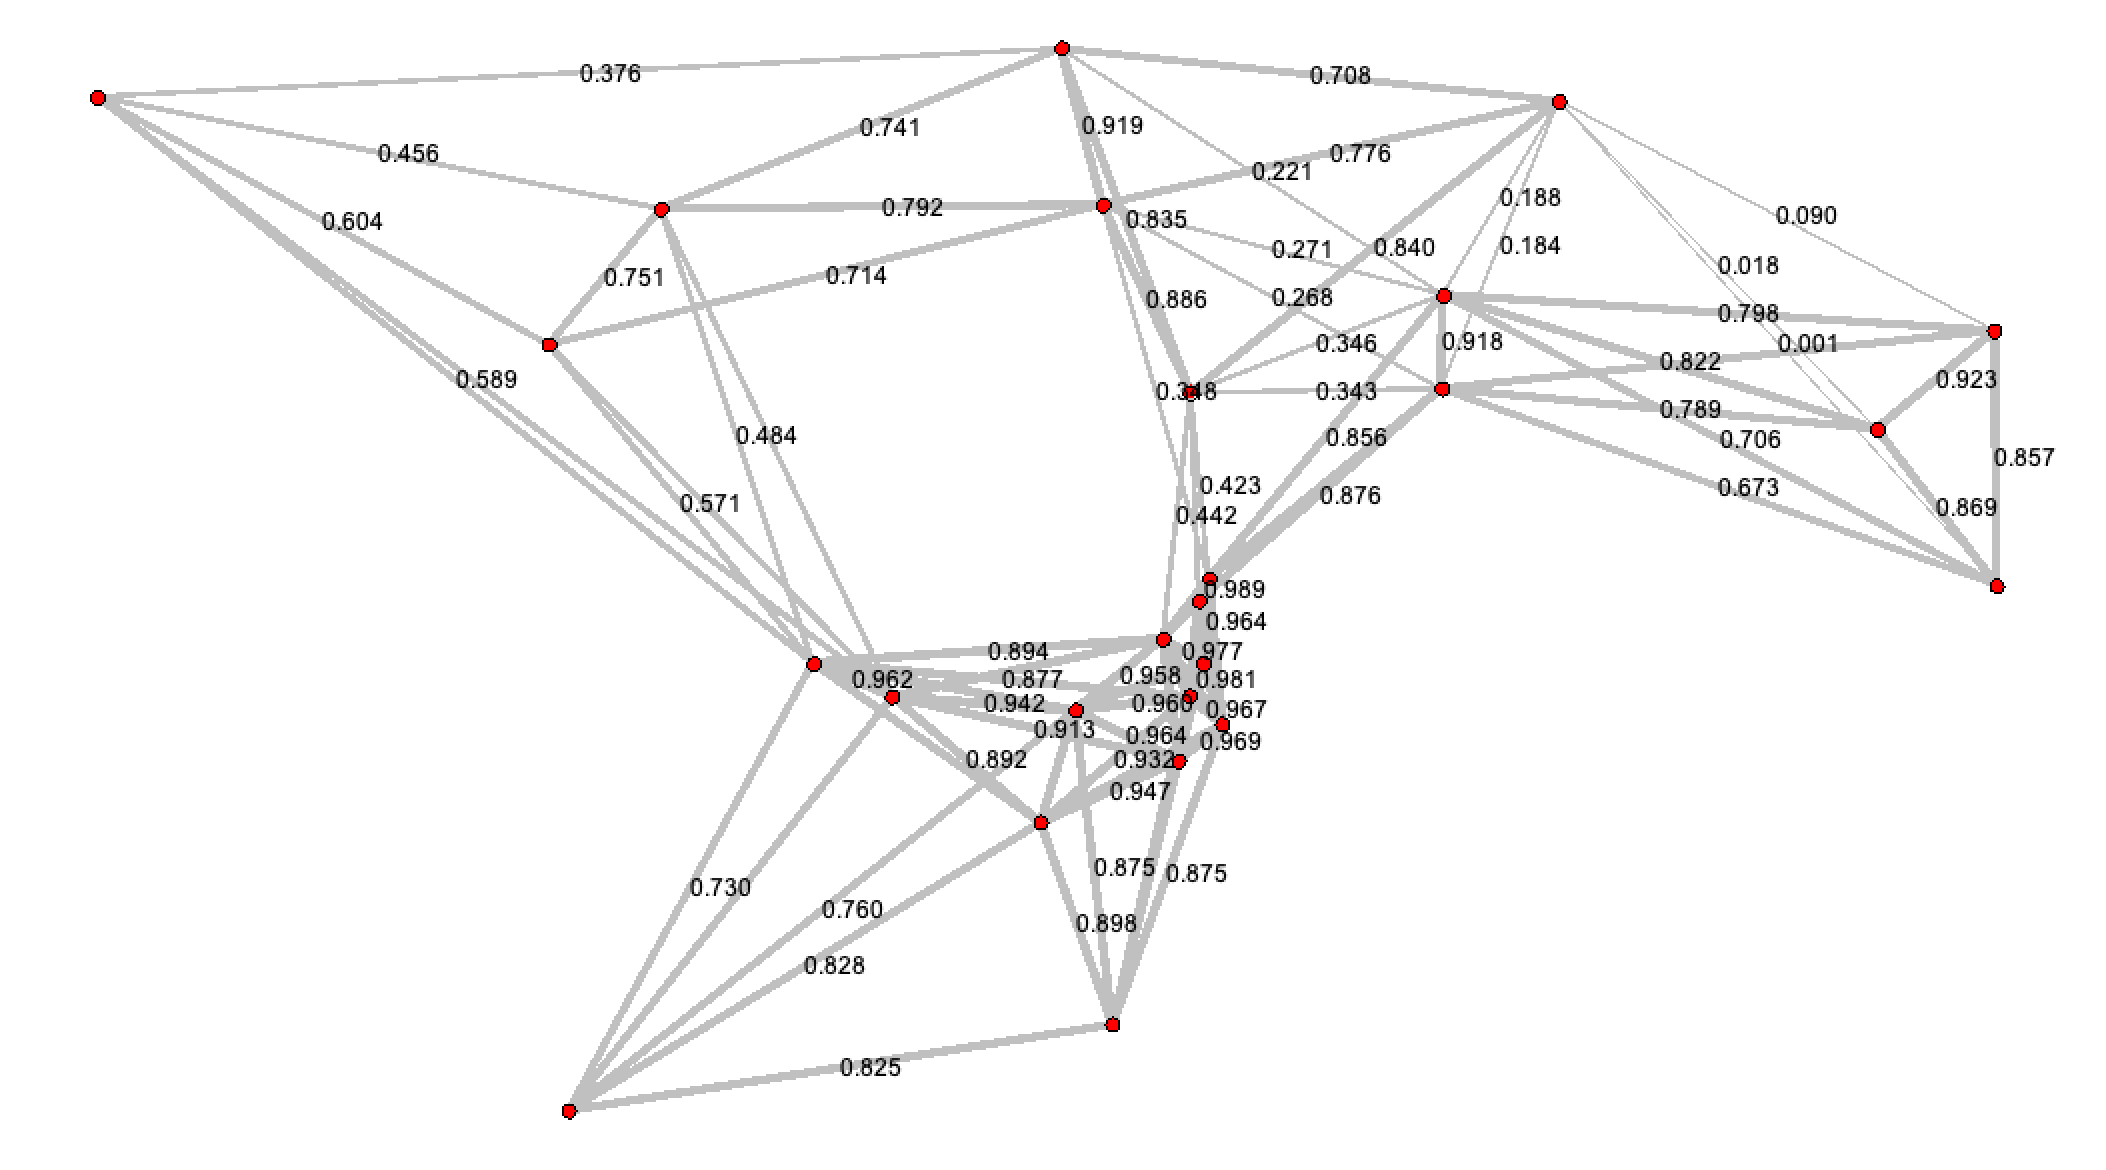
\includegraphics[width=0.6\textwidth]{img/k_nearest}
\caption{K-Nearest Neighbors graph with $k=5$ applied to student location data. Each point is connected to its five closest neighbors, creating a sparse network that preserves local connectivity while significantly reducing the number of edges compared to the complete graph.}
\label{fig:knn_graph}
\end{figure}

\section{Clustering Graph Representation of IZTECH}
\label{sec:clustering_graph}

Once the various graph representations were constructed, we applied clustering algorithms to partition the nodes (students) into clusters, representing potential bus routes. The clustering phase is critical for identifying cohesive groups of students who can be efficiently transported together.

\subsection{Clustering Complete Graph Representation}
\label{subsec:clustering_complete}

Clustering the complete graph representation presents unique challenges due to its dense connectivity. Our implementation applies multiple clustering algorithms to the complete graph, each configured to respect the bus capacity constraints. We enforced a minimum cluster size of 10 students (minimum efficient bus occupancy) and a maximum cluster size of 50 students (maximum bus capacity) to ensure practical viability of the resulting routes.

\begin{figure}[!htbp]
\centering
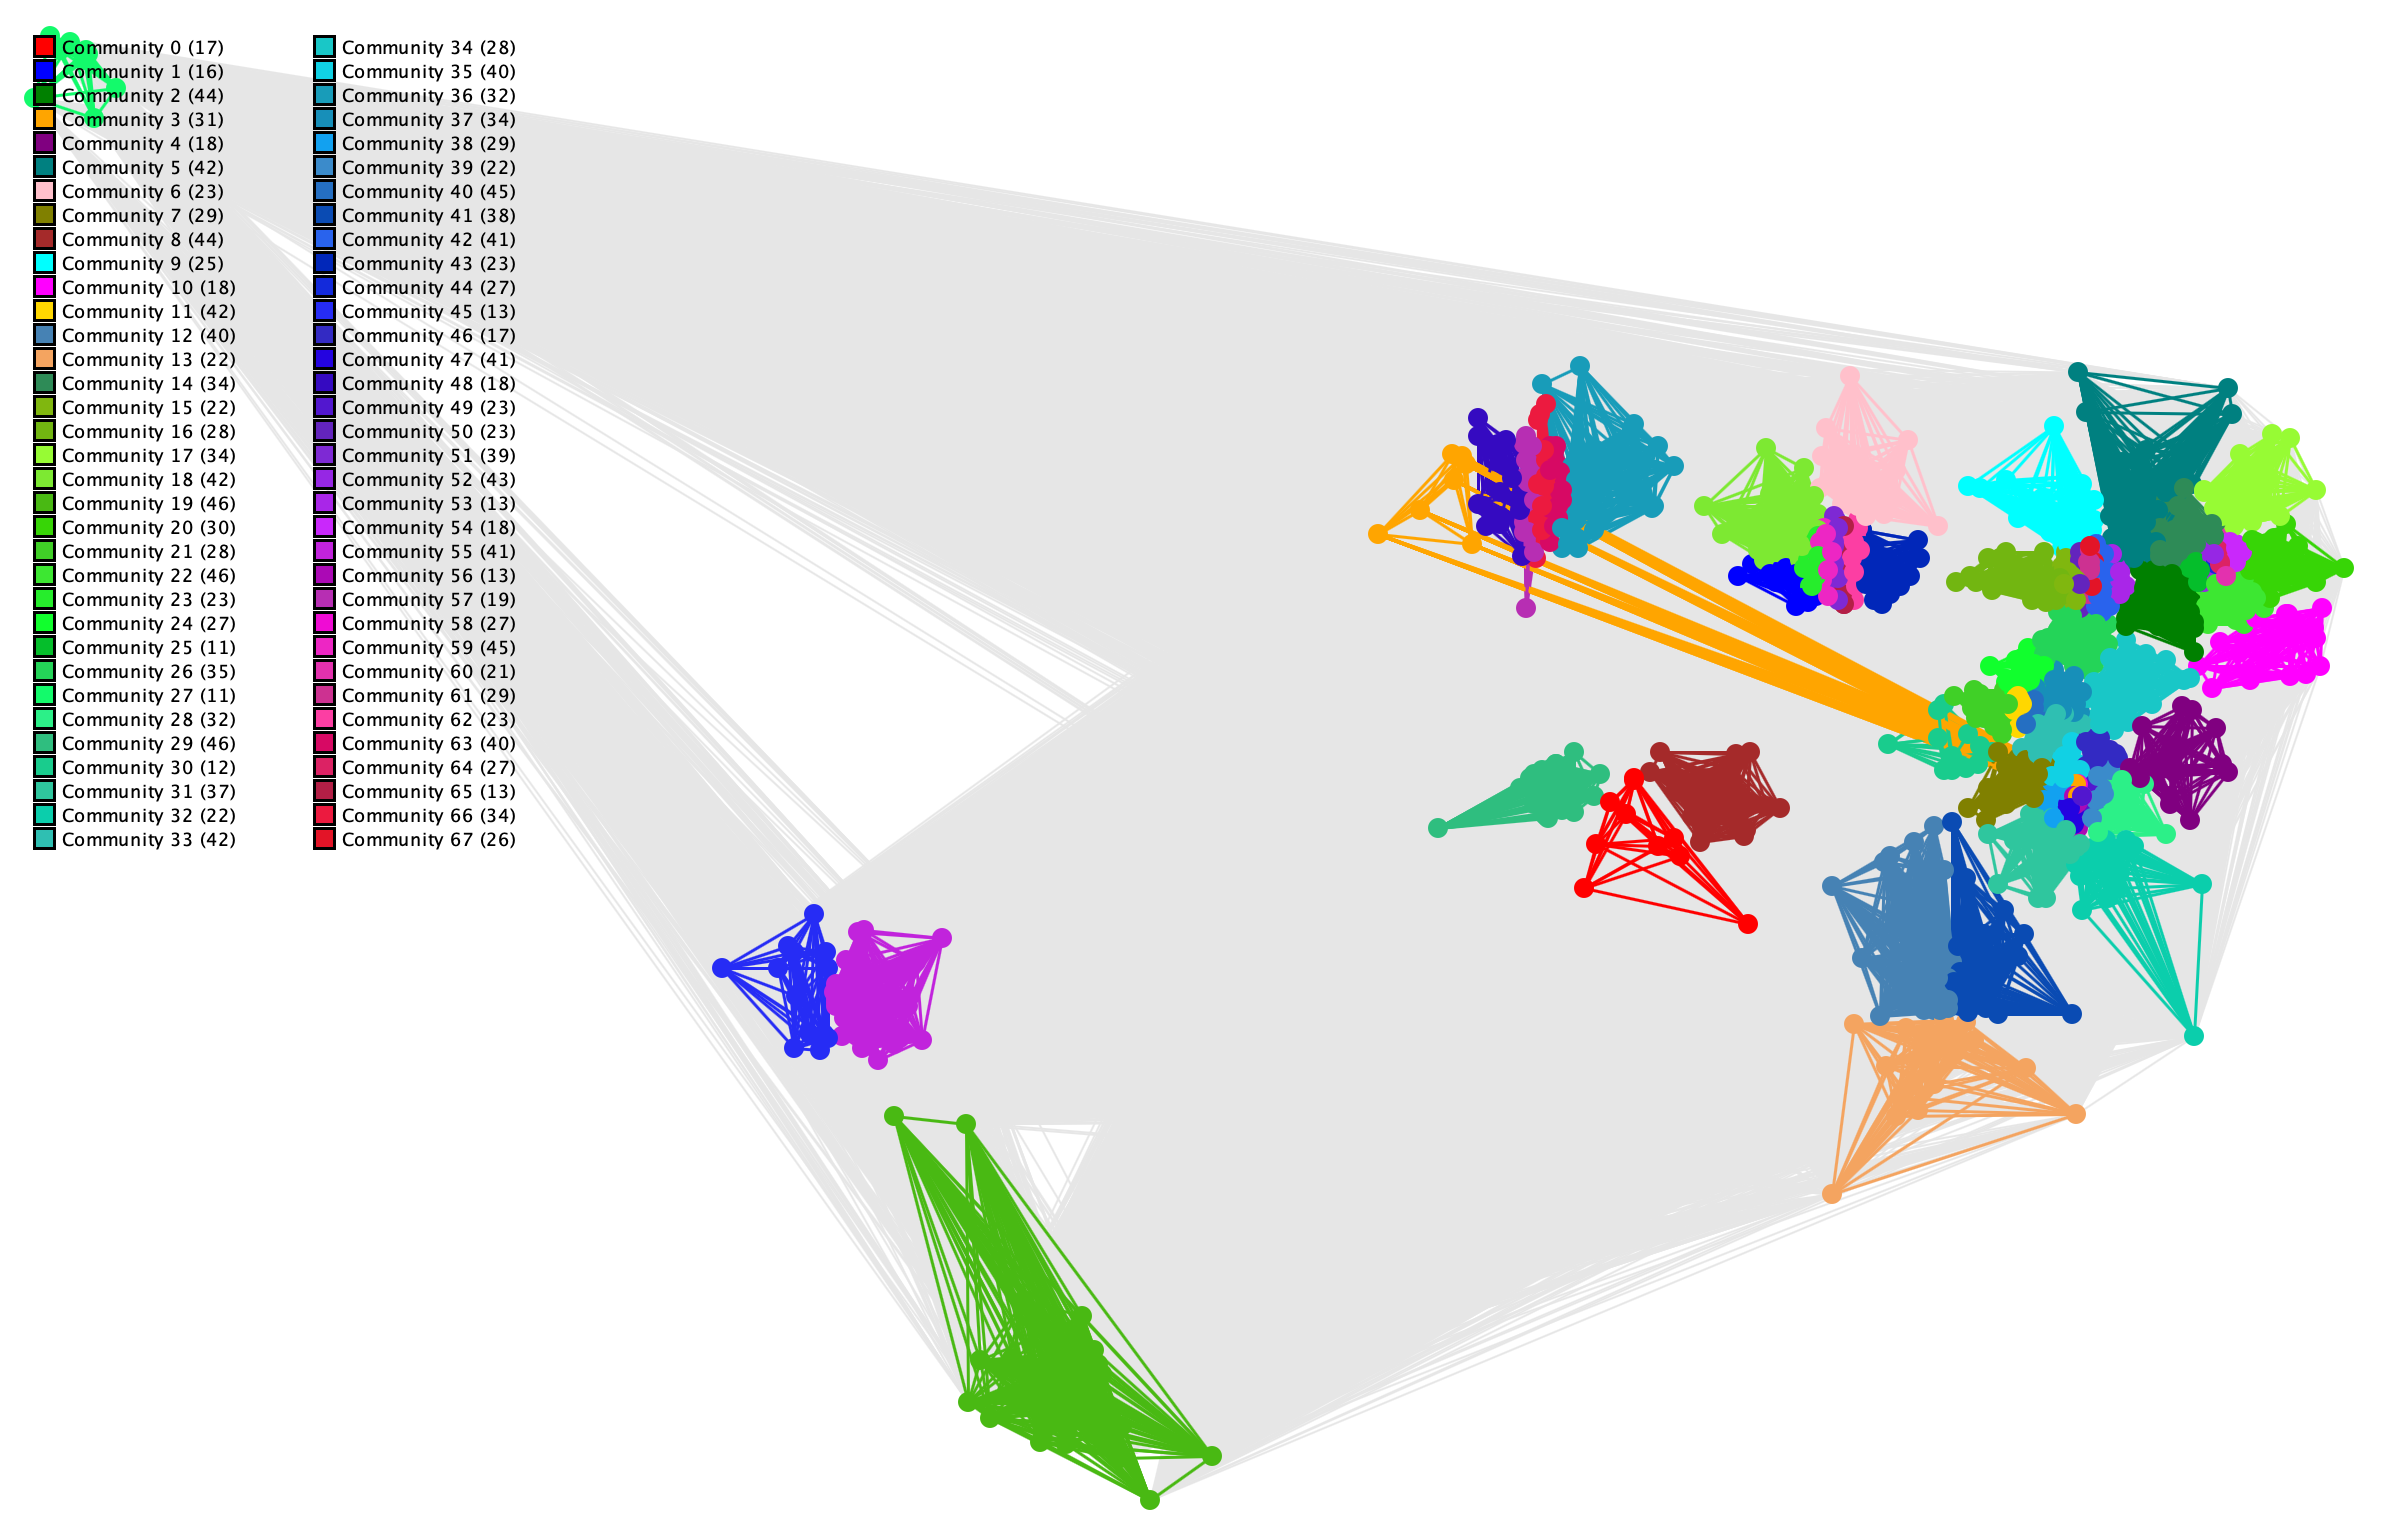
\includegraphics[width=0.8\textwidth]{img/leiden_complete2}
\caption{Leiden algorithm applied to a complete graph representation. The high number of edges between all student locations illustrates the computational expensiveness of the complete graph approach, making it less practical for large-scale transportation planning.}
\label{fig:leiden_complete}
\end{figure}

We primarily utilized the Leiden algorithm (see Section~\ref{subsec:LeidenAlgorithm}), which optimizes modularity to find densely connected communities with its refinement phase ensuring well-connected clusters. The algorithm was configured with adaptive resolution to produce balanced clusters.

\begin{table}[h]
\centering

\label{tab:leiden_complete_example}
\begin{tabular}{|c|c|c|c|c|c|c|c|}
\hline
\textbf{Comm.} & \textbf{Students}  &  \textbf{Distance} & \textbf{Fuel} & \textbf{Fuel Cost} & \textbf{Total} \\
\textbf{ID} & & \textbf{(km)} & \textbf{(L)} & \textbf{(TL)} & \textbf{Cost (TL)} \\
\hline
54 & 18  & 45.70 & 18.74 & 849.35 & 2445.35 \\
\hline
\end{tabular}
\caption{Example of a clustered community using Leiden algorithm on complete graph}
\end{table}

The clusters from the complete graph often required post-processing to merge small communities and split oversized ones, ensuring adherence to the capacity constraints. This post-processing uses geographic proximity to guide the merging and splitting operations, prioritizing the combination of communities that are spatially close while ensuring each resulting community remains within the capacity limits.

\subsubsection{Minibus Solution for Imbalanced Clusters}
\label{subsubsec:minibus_solution}

When analyzing the complete graph representation, we observed that the resulting clusters were often imbalanced, with many clusters having fewer than 25 students. This created an inefficiency in the transportation system, as standard buses with a capacity of 50 students would be underutilized. To address this issue, we implemented a vehicle type allocation strategy that assigns minibuses (with a maximum capacity of 25 students) to smaller clusters containing 10-25 students, while standard buses were allocated to larger clusters with 26-50 students. This differentiated approach resulted in significant cost savings due to the lower fuel consumption of minibuses compared to standard buses. However, it's important to note that IZTECH currently does not have minibuses in its fleet, only standard buses. This limitation motivates our exploration of alternative graph construction methods that might produce more balanced clusters suitable for the existing bus fleet.

\subsection{Clustering Sparse Graph Representation}
\label{subsec:clustering_sparse}

The sparse graph representations required specialized clustering approaches to effectively partition the transportation network. In our implementation, each node in the graph represents a specific student's residential address in Izmir, with geographical coordinates (latitude and longitude) obtained from our synthetic dataset. The edges represent potential transportation links between student locations, with weights based on the Euclidean distance between points.

For our transportation network analysis, we implemented three clustering algorithms with specific configurations tailored to the IZTECH student transportation problem. All implementations included specialized vehicle allocation logic that assigns buses with our capacity constraints (10-50 students per bus), optimizing for both fleet size and route efficiency.

\subsubsection{Performing Spectral Clustering on Sparse Graph Representations of IZTECH}
\label{subsubsec:spectral_implementation}

For the Spectral clustering implementation, we focused on optimizing the eigendecomposition process for large sparse matrices. Our implementation used the normalized Laplacian matrix and employed an adaptive approach to determine the number of clusters. We developed a custom post-processing step that enforces our specific bus capacity constraints (10-50 students) by iteratively merging small clusters or splitting oversized ones based on geographic proximity.

\begin{figure}[htbp]
\centering
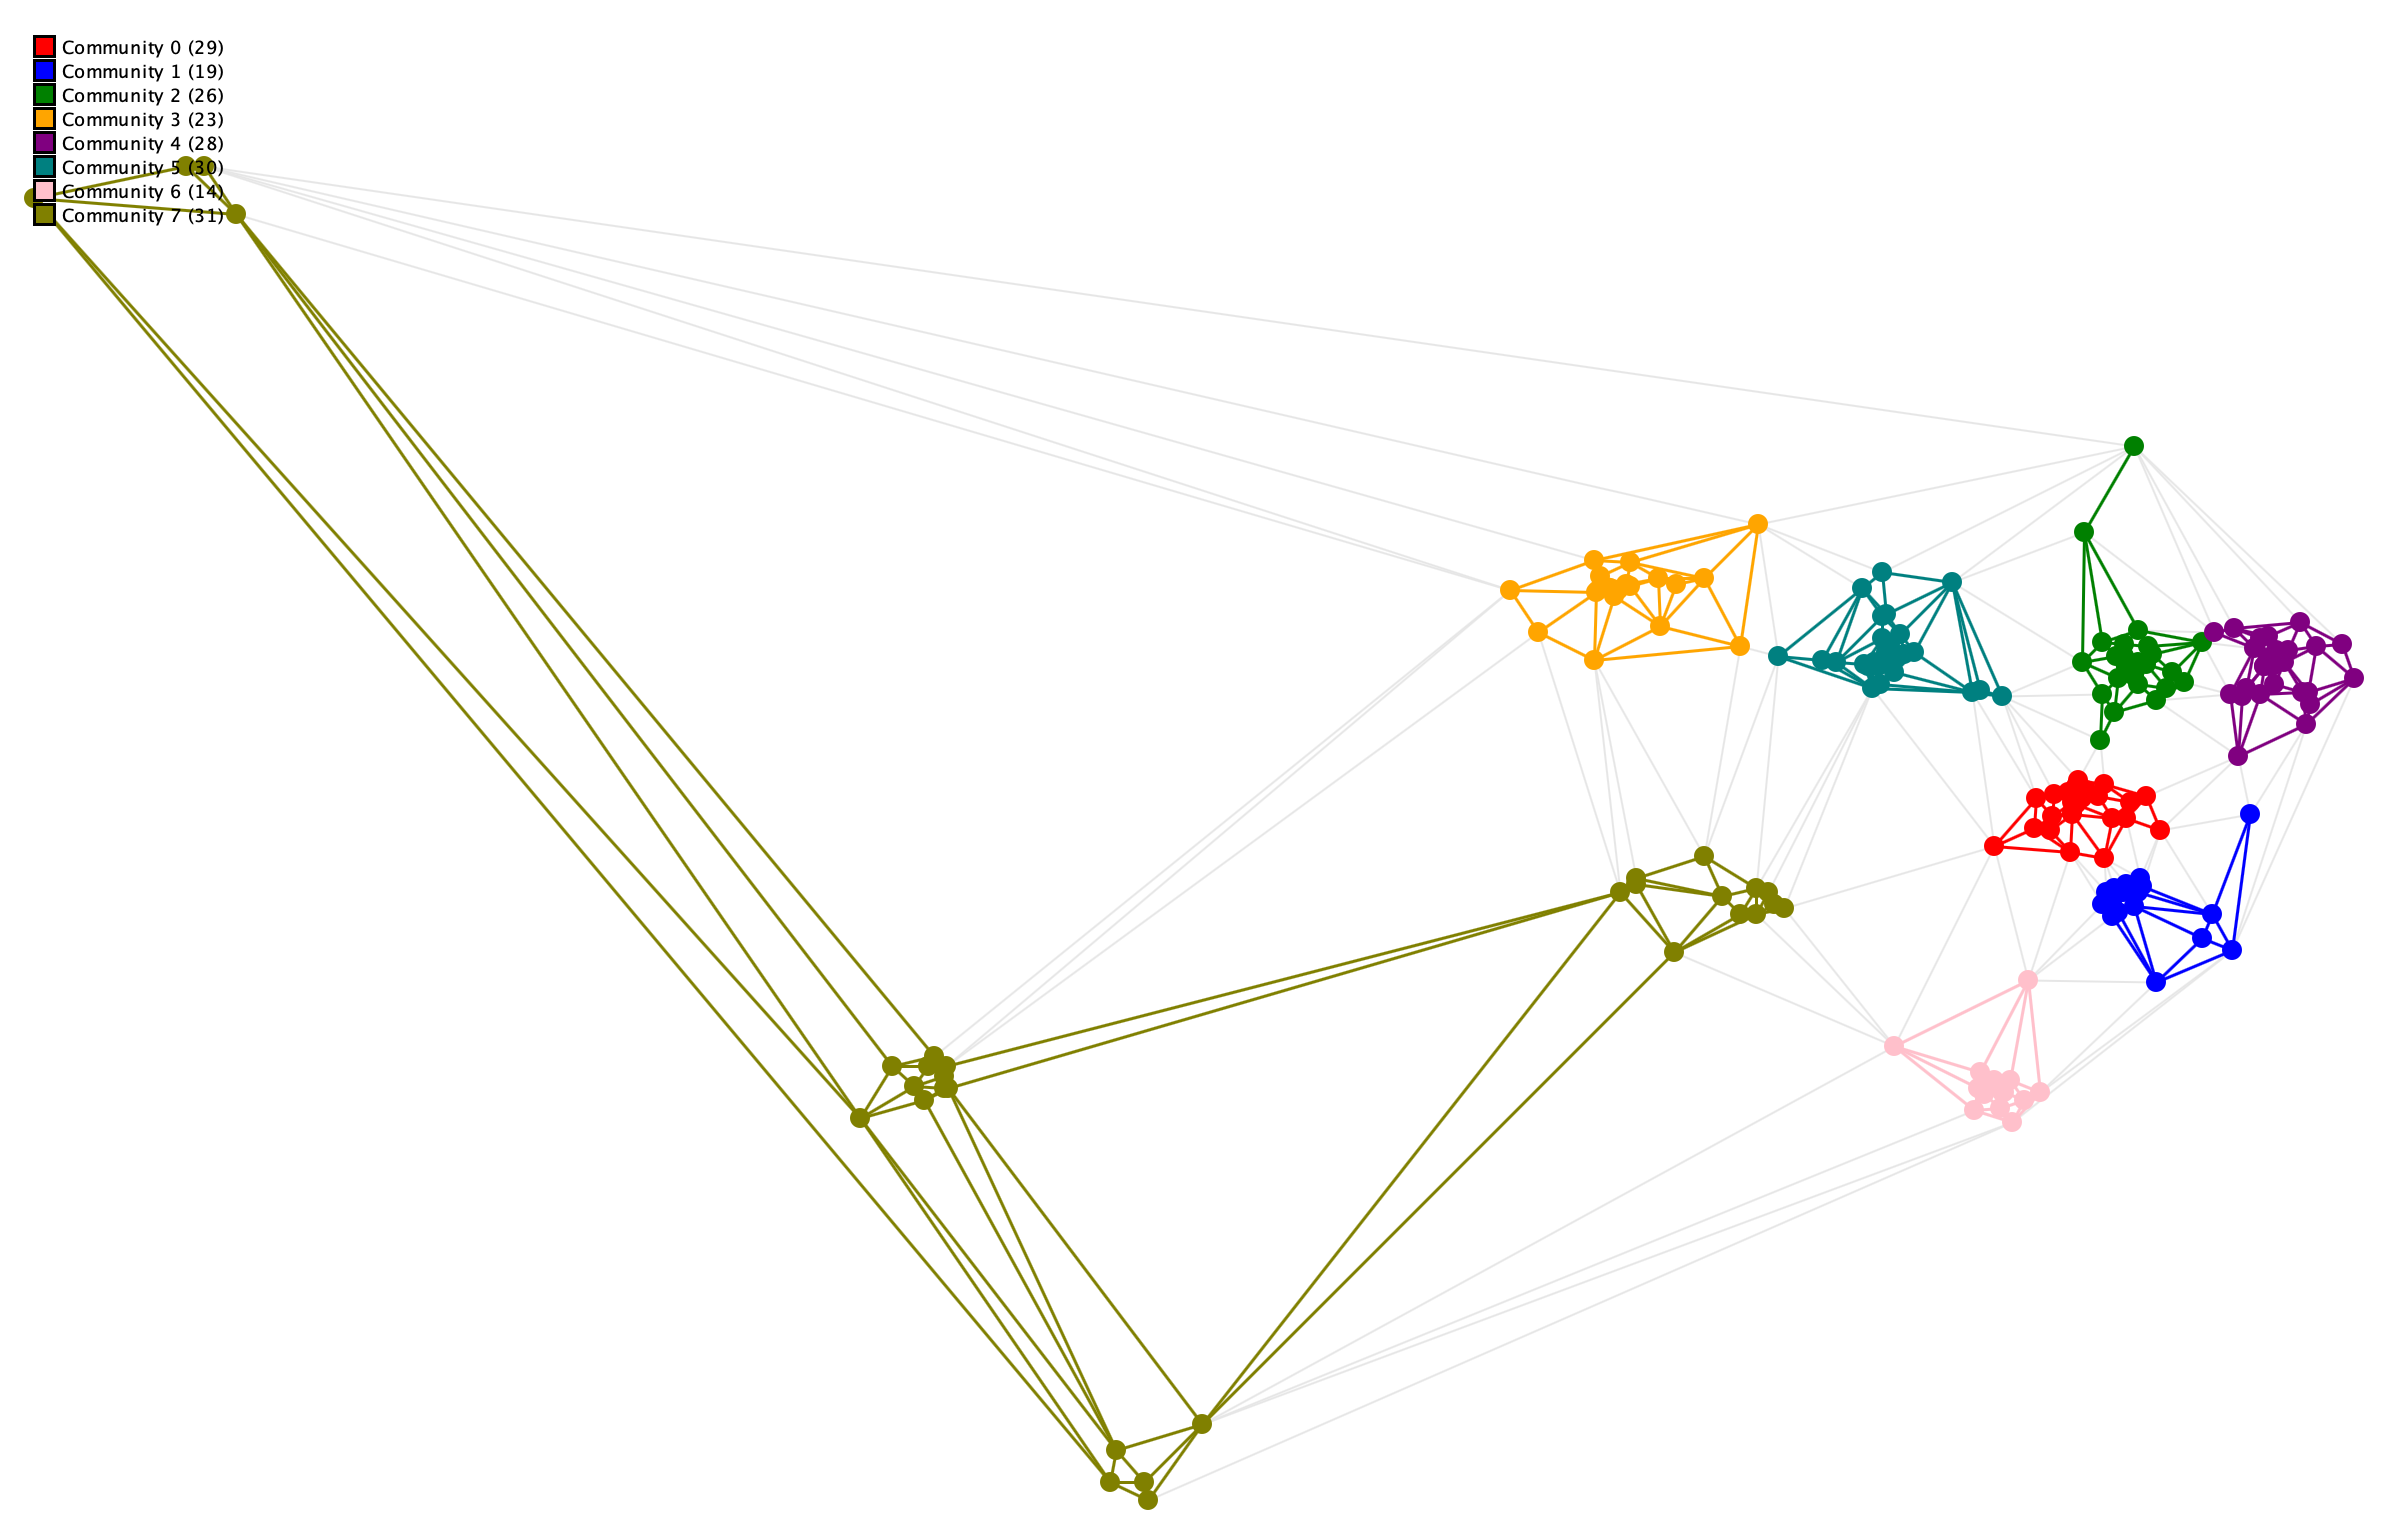
\includegraphics[width=0.7\textwidth]{./img/Spectral_Delaunay}
\vspace{0.5cm}

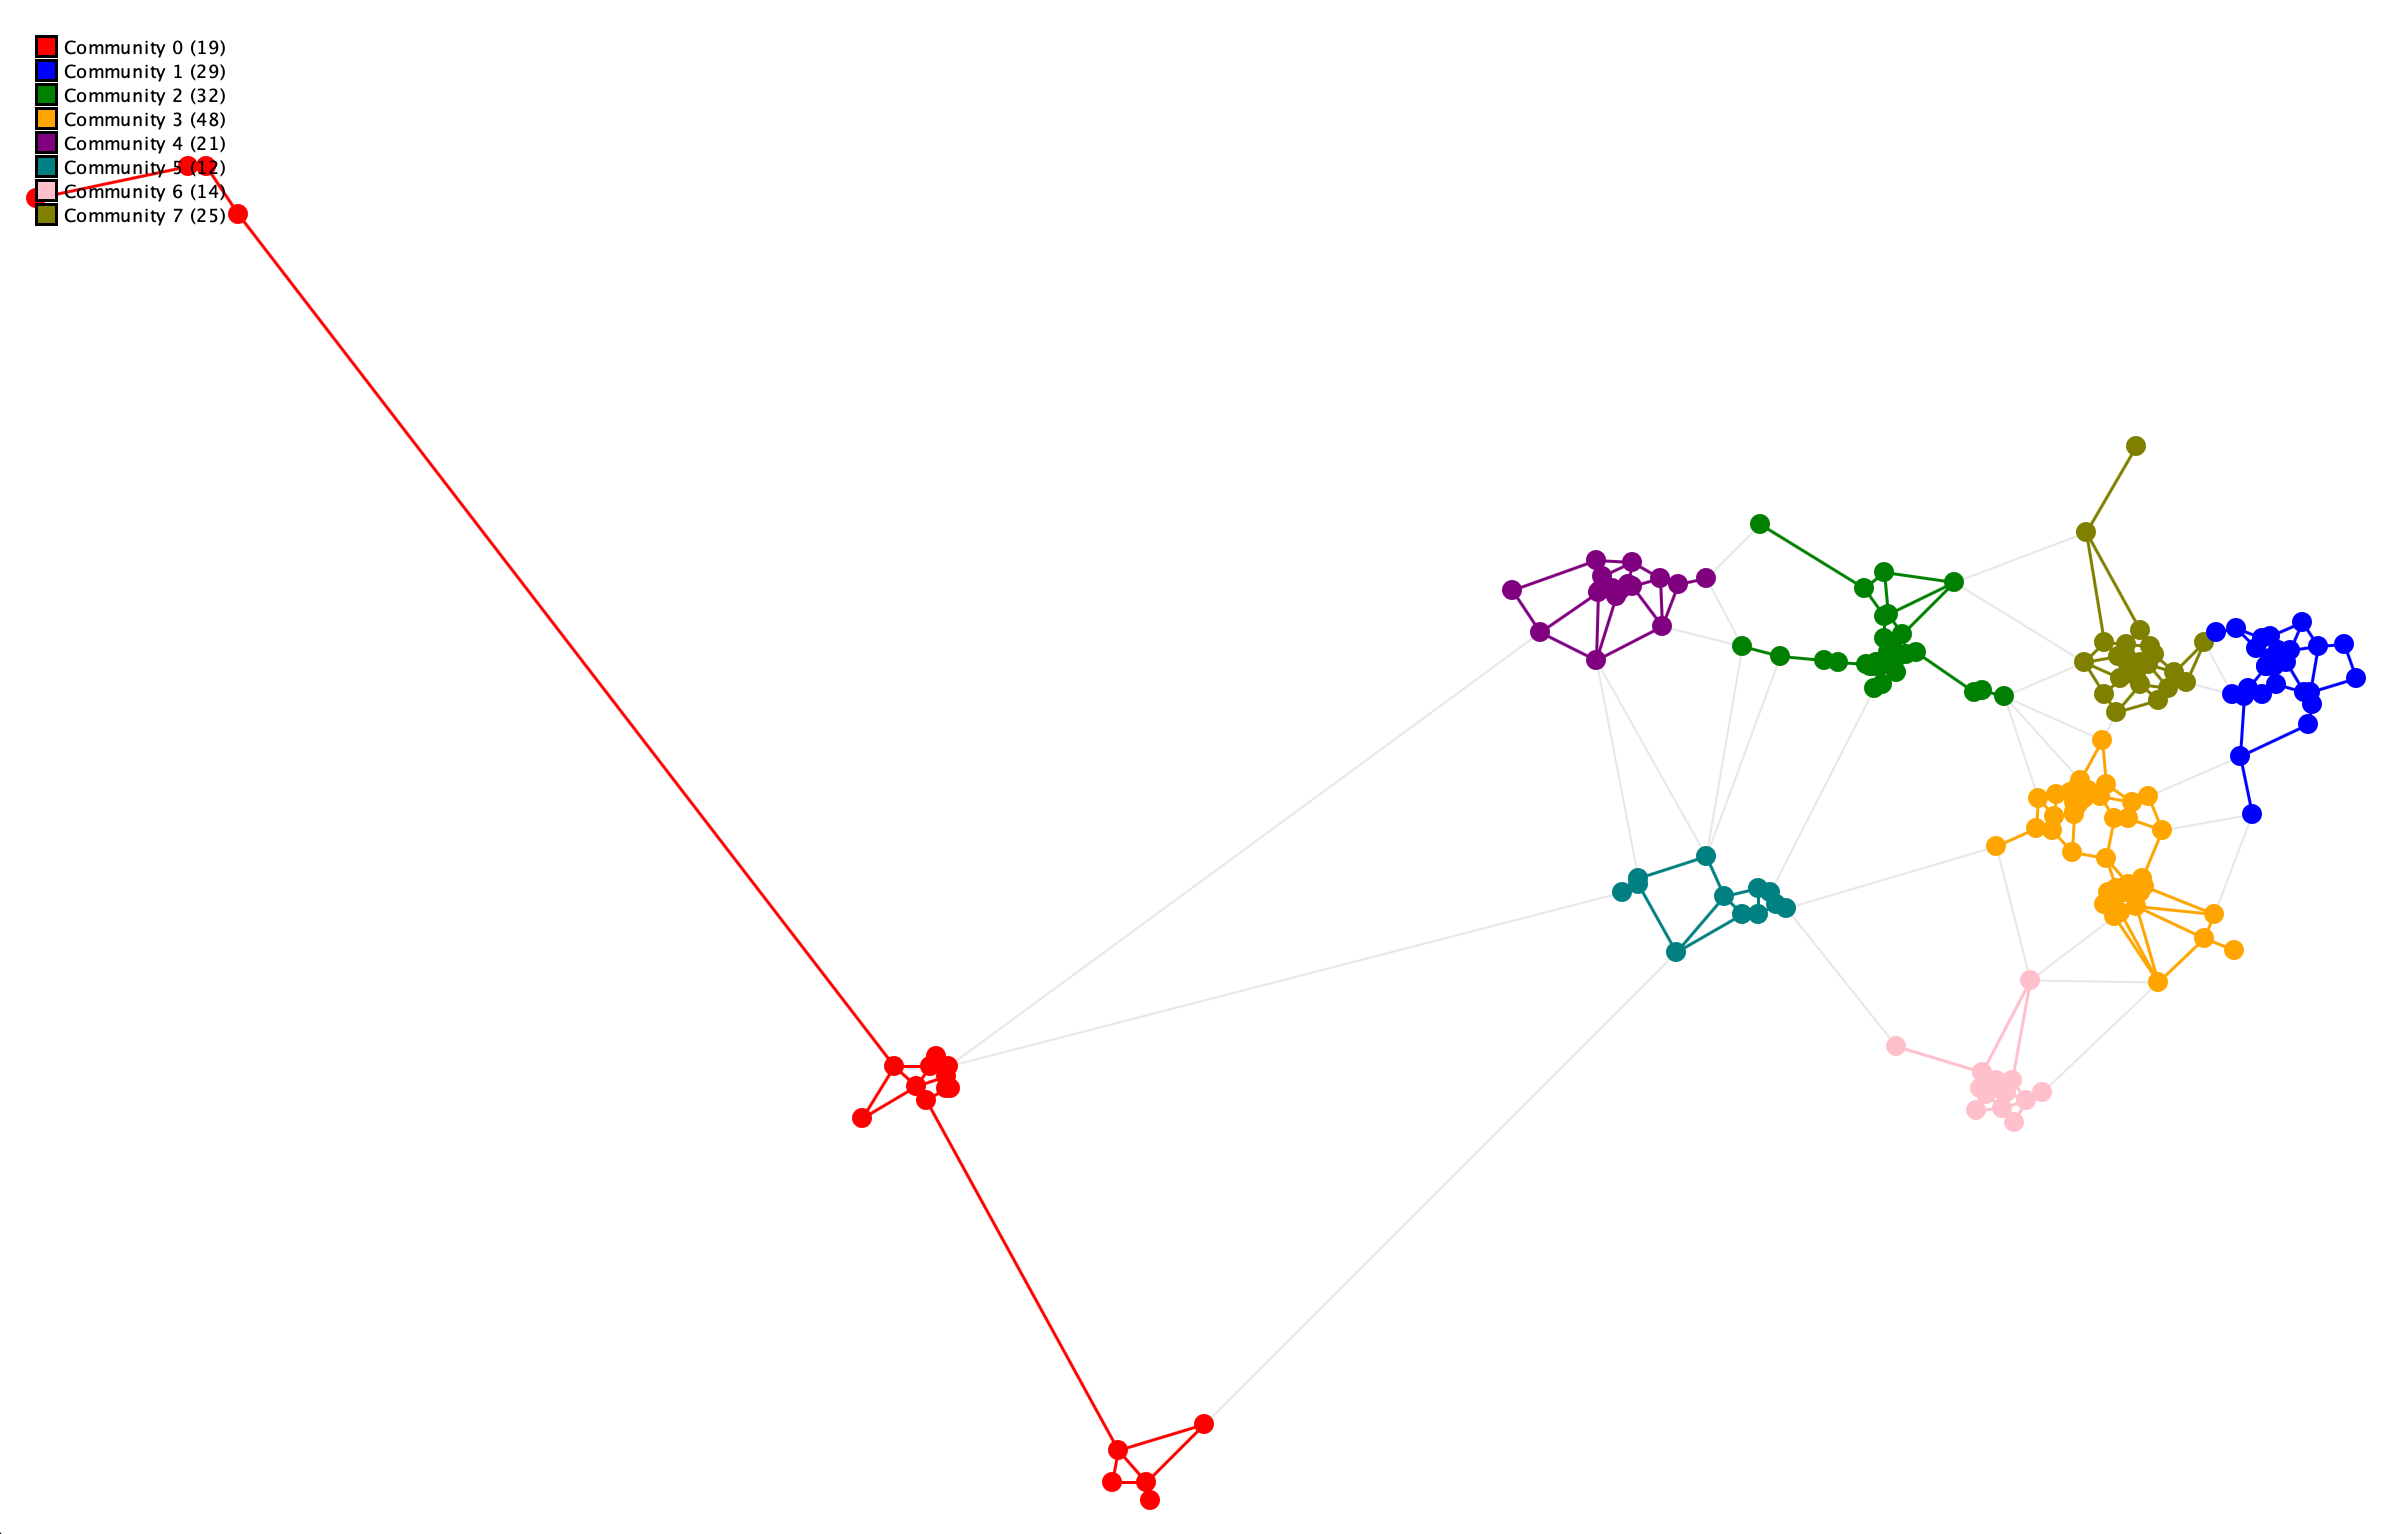
\includegraphics[width=0.7\textwidth]{./img/Spectral_Gabriel}
\vspace{0.5cm}

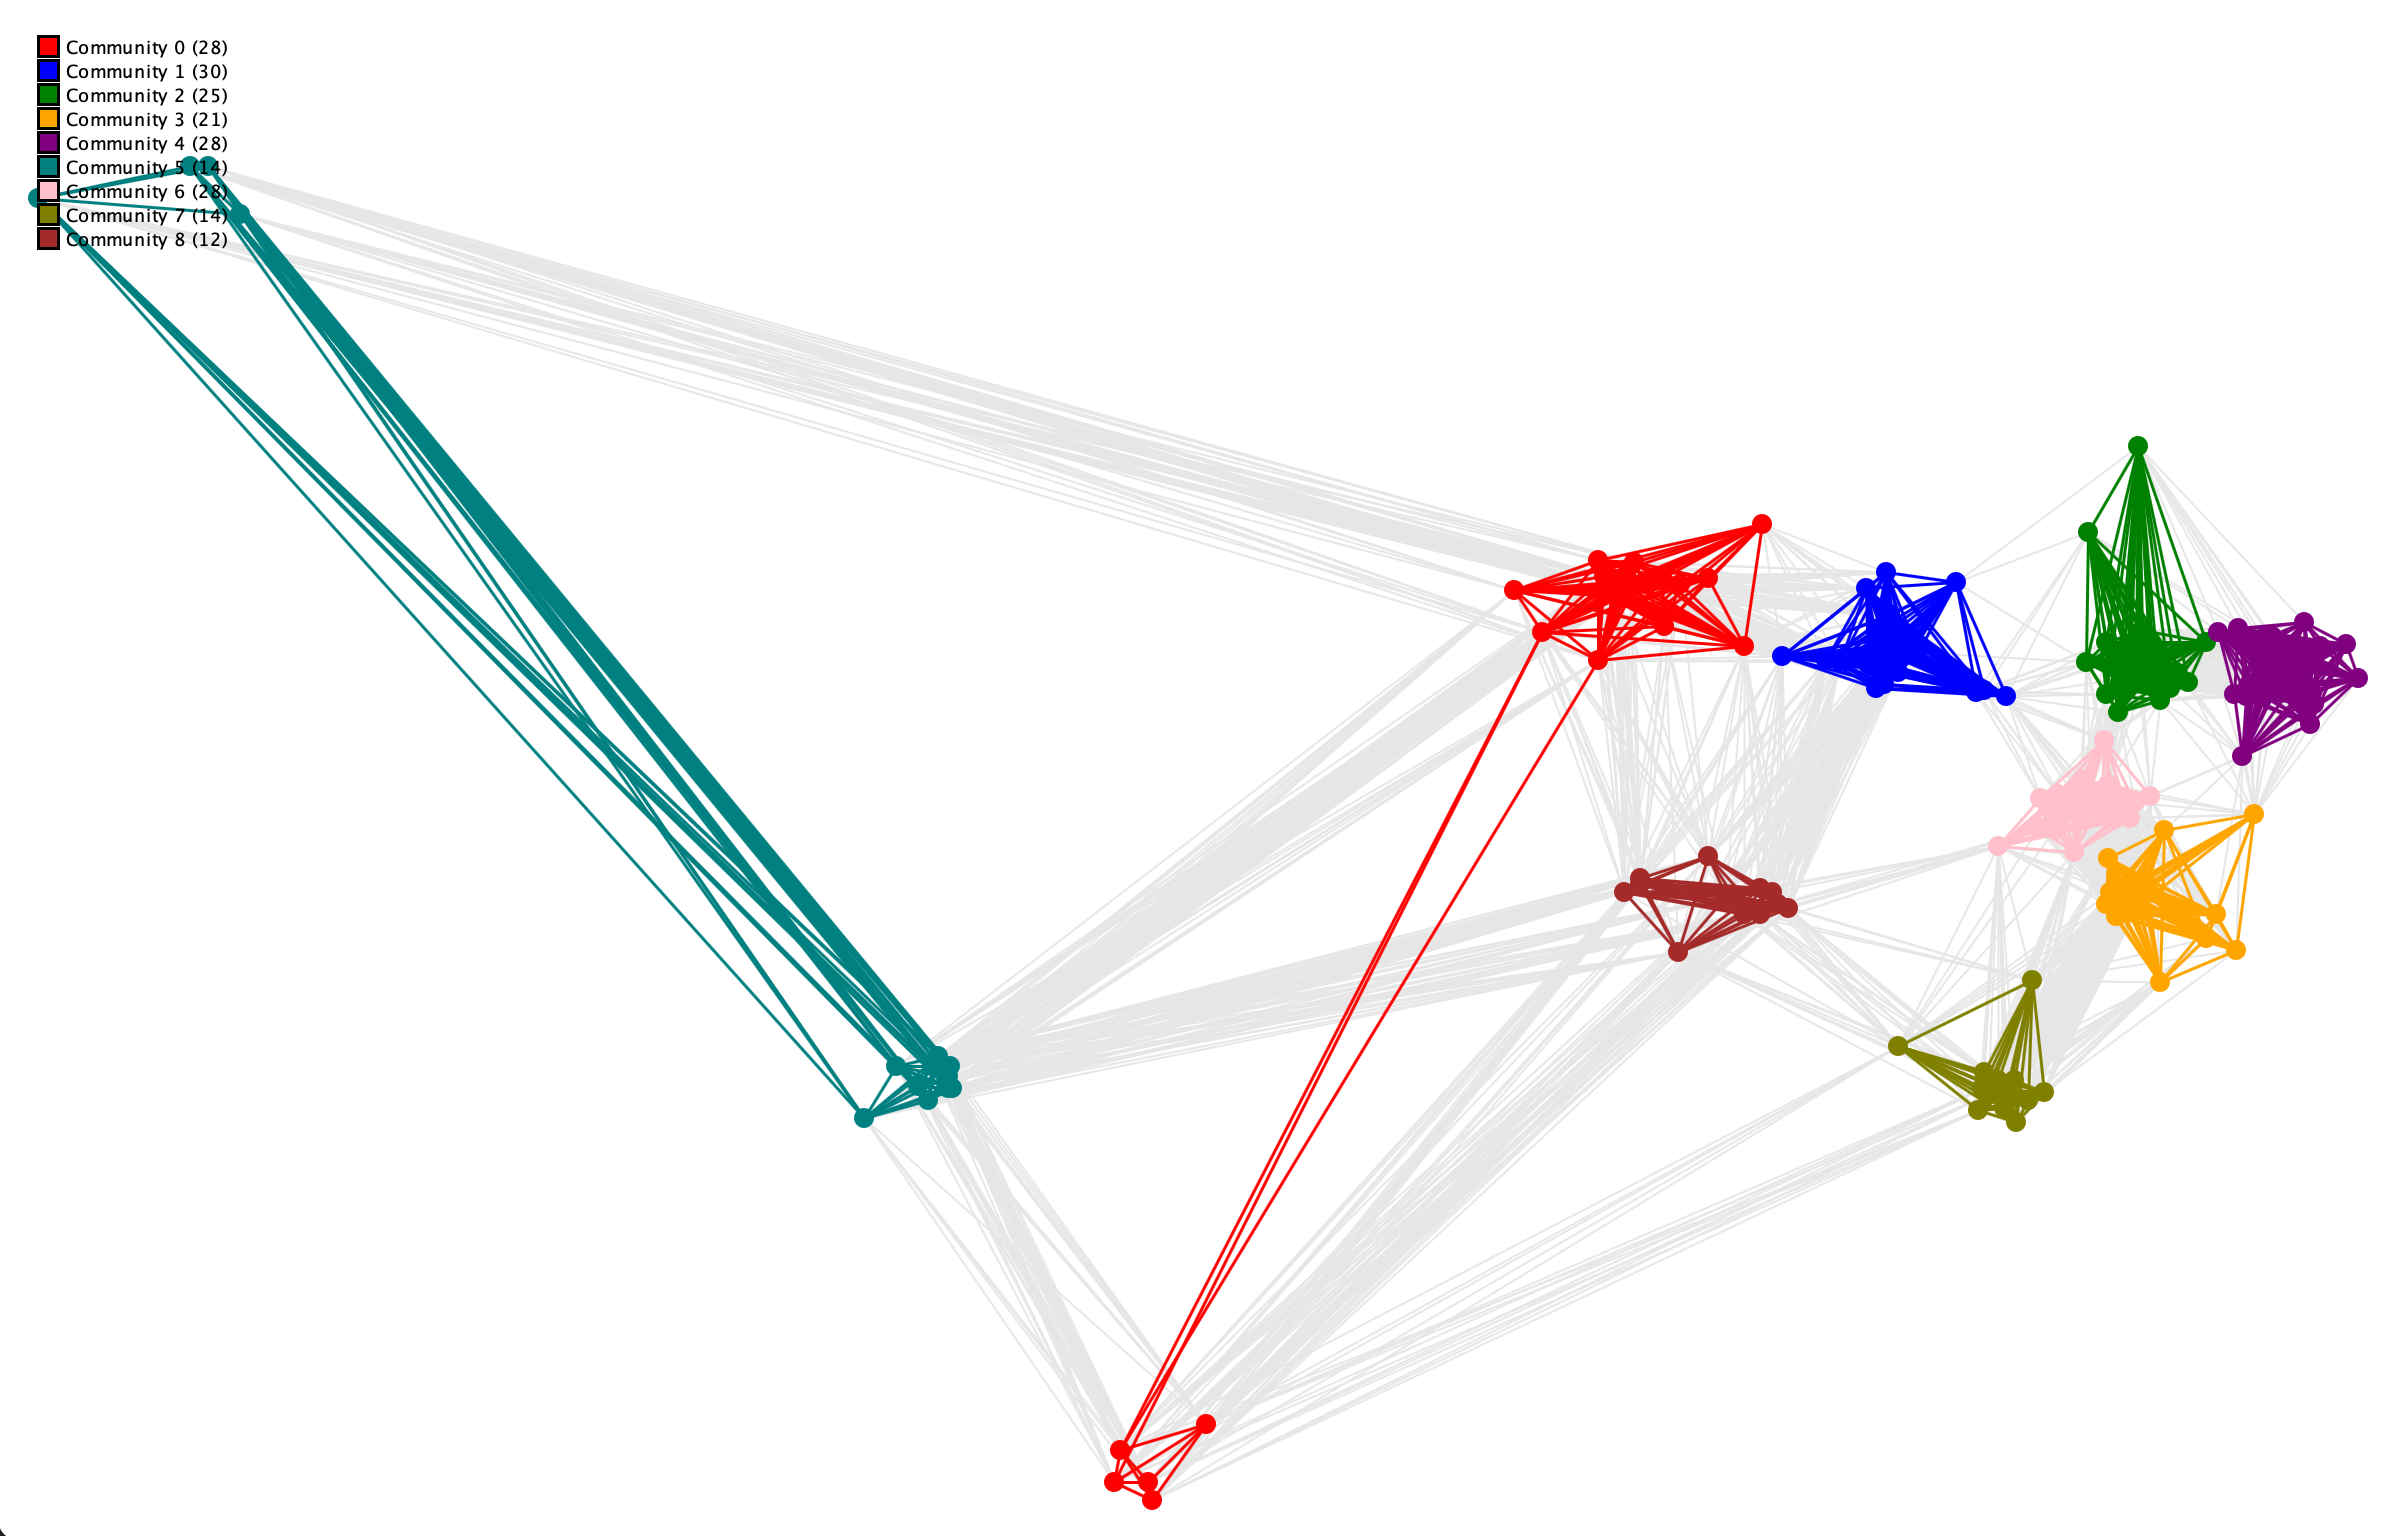
\includegraphics[width=0.7\textwidth]{./img/Spectral_K}

\caption{Spectral clustering applied to different sparse graph representations (top: Delaunay, middle: Gabriel, bottom: K-Nearest) with 200 student locations.}
\label{fig:spectral_clustering}
\end{figure}

Figure \ref{fig:spectral_clustering} illustrates the application of Spectral clustering to three different sparse graph representations. Each point represents a student address, and colors indicate cluster assignments. With Delaunay triangulation, clusters form well-connected regions with smoother boundaries; with Gabriel graph, clusters are more compact but show increased fragmentation; with K-Nearest Neighbors (k=30), clusters demonstrate better local coherence but with some outlier assignments.

As shown in these visualizations, our Spectral clustering implementation tends to create clusters with clear geographical boundaries. This demonstrates how the algorithm's eigenvalue-based dimensionality reduction effectively captures the global structure of Izmir's transportation network. The clusters formed by spectral clustering typically have larger student counts, which aligns with the algorithm's natural tendency to identify major structural divisions in the graph before finer details.

The spectral approach is particularly suitable for transportation planning scenarios that prioritize minimizing the number of vehicles while accepting potentially longer routes per vehicle.

\subsubsection{Performing Leiden Clustering on Sparse Graph Representations of IZTECH}
\label{subsubsec:leiden_implementation}

For the Leiden algorithm implementation, we modified the original algorithm to better handle transportation constraints. Specifically, we incorporated a custom quality function that considers both community modularity and geographic compactness. We adjusted the resolution parameter based on the sparsity of the underlying graph, with values ranging from 0.8 for complete graphs to 1.2 for sparser representations. This adaptation allowed the algorithm to find well-connected communities while respecting the spatial constraints inherent in transportation planning.

\begin{figure}[htbp]
\centering
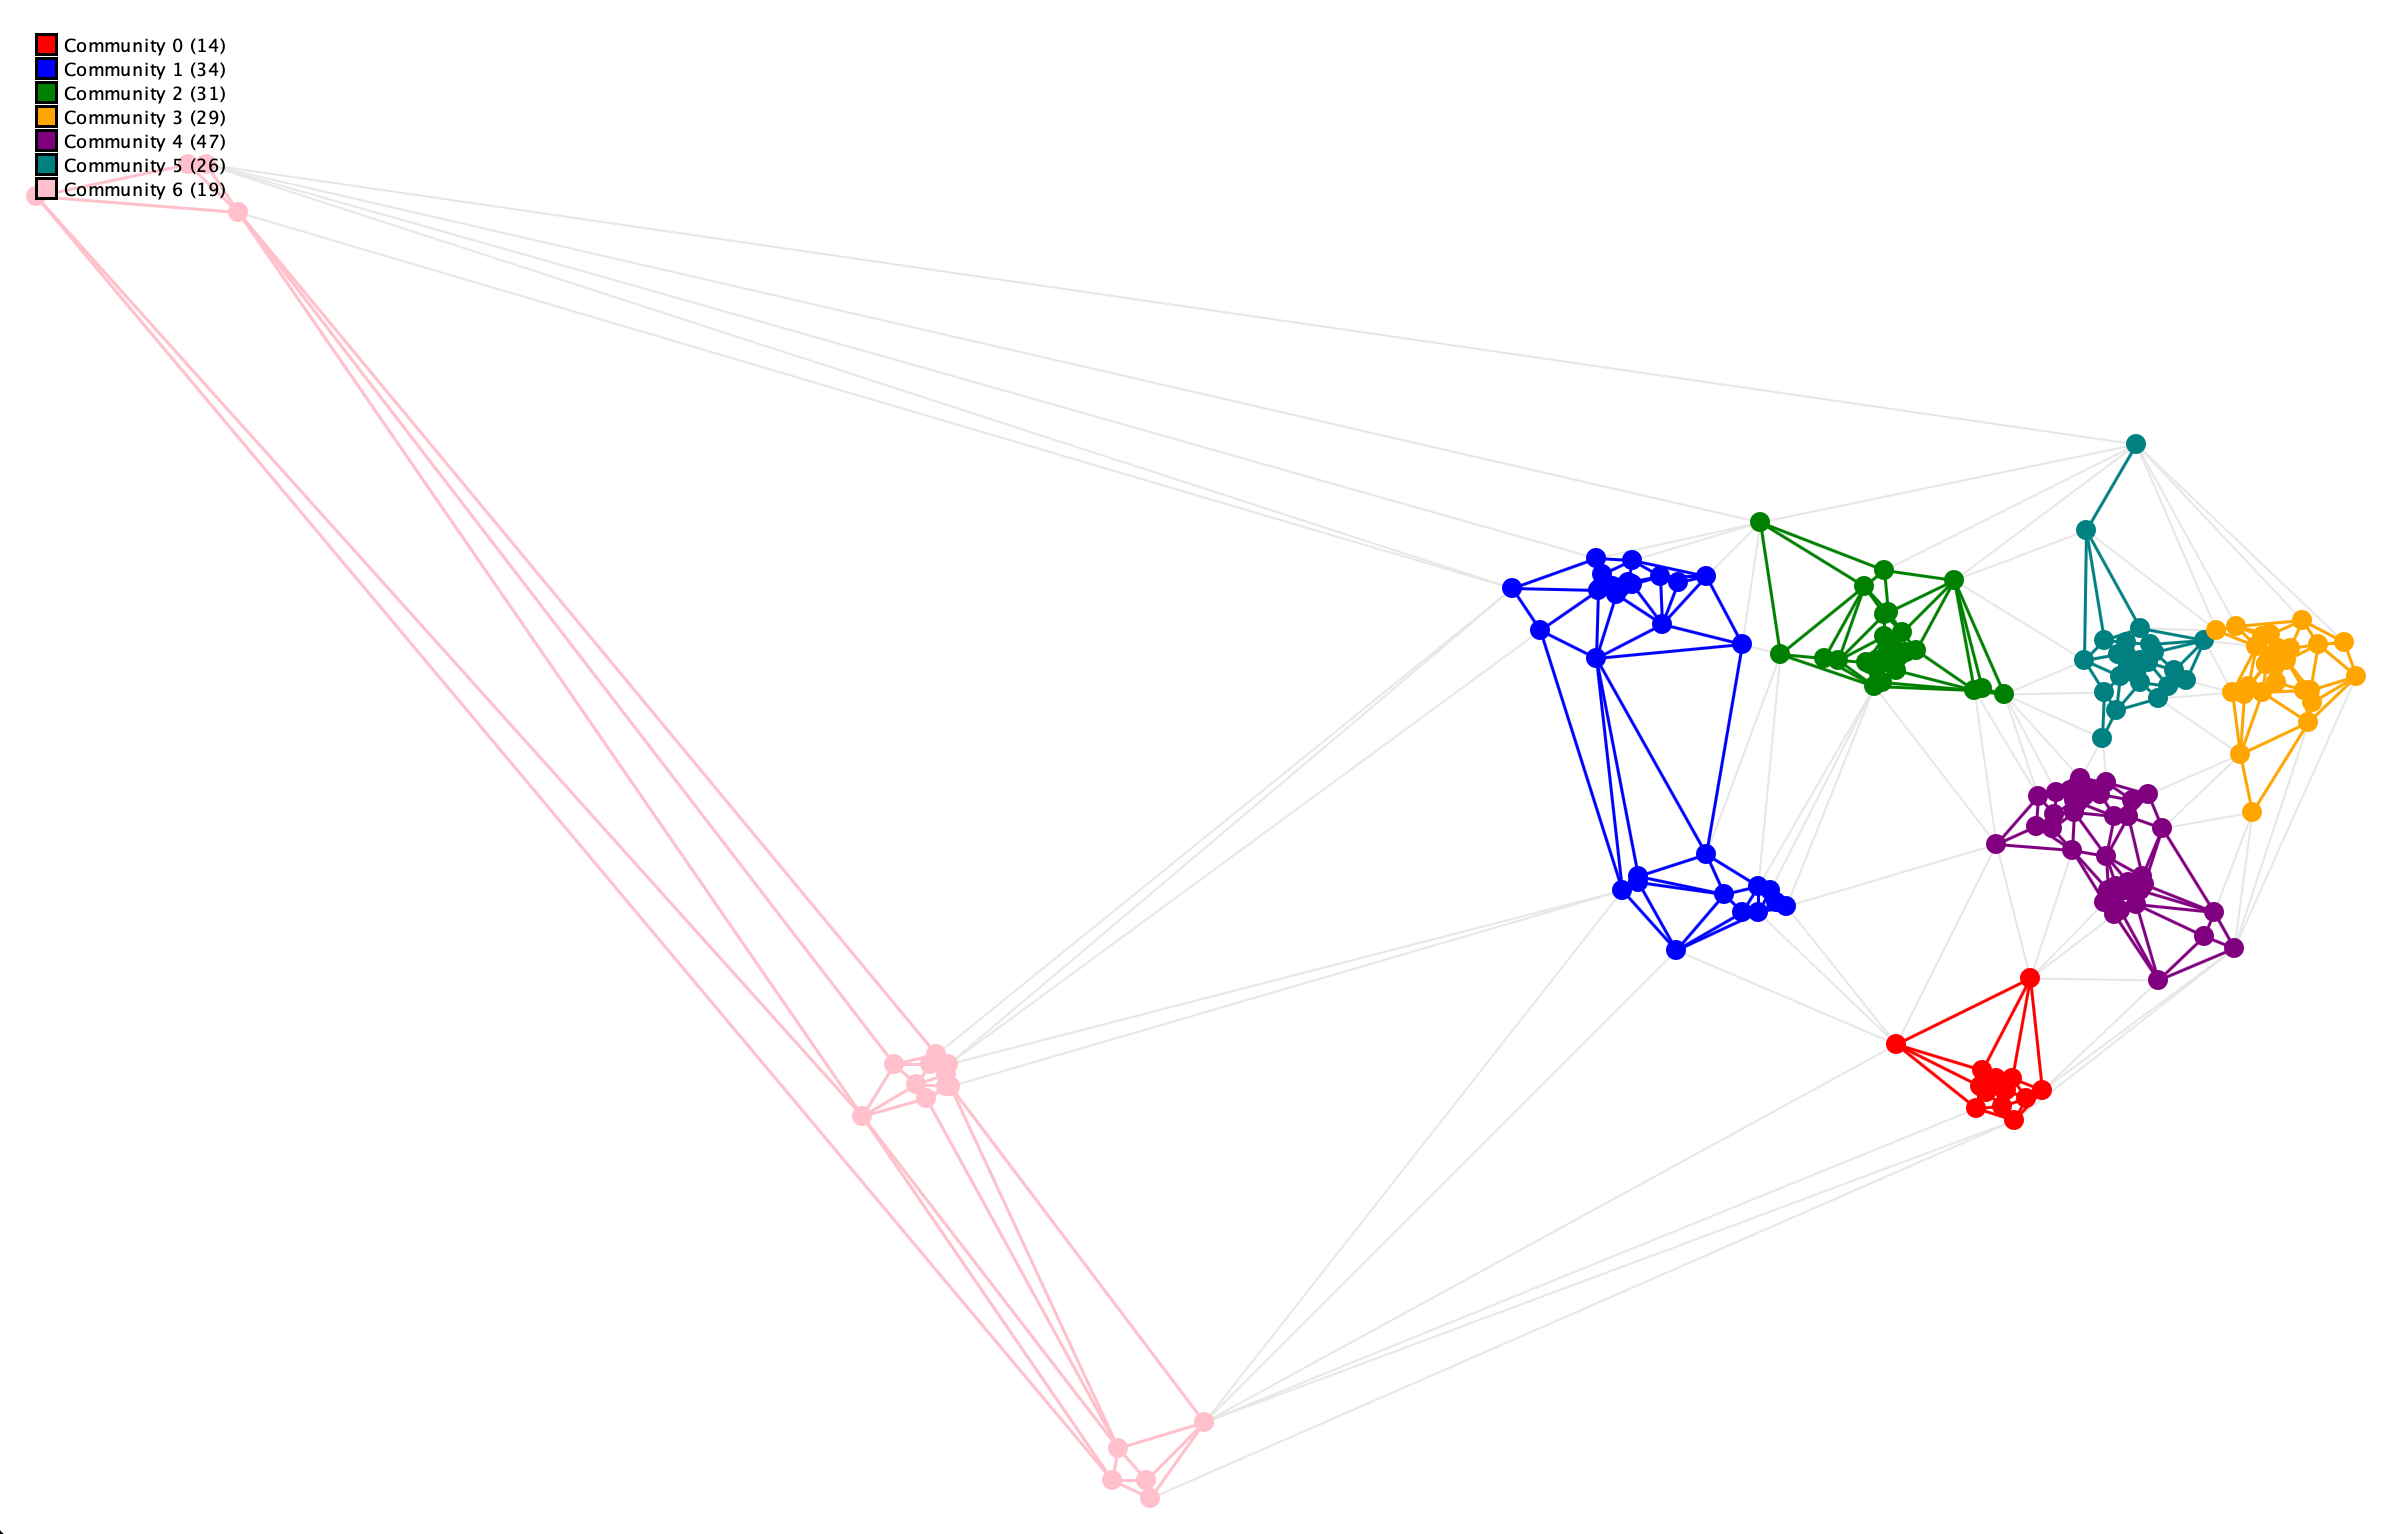
\includegraphics[width=0.7\textwidth]{./img/Leiden_Delaunay}
\vspace{0.5cm}

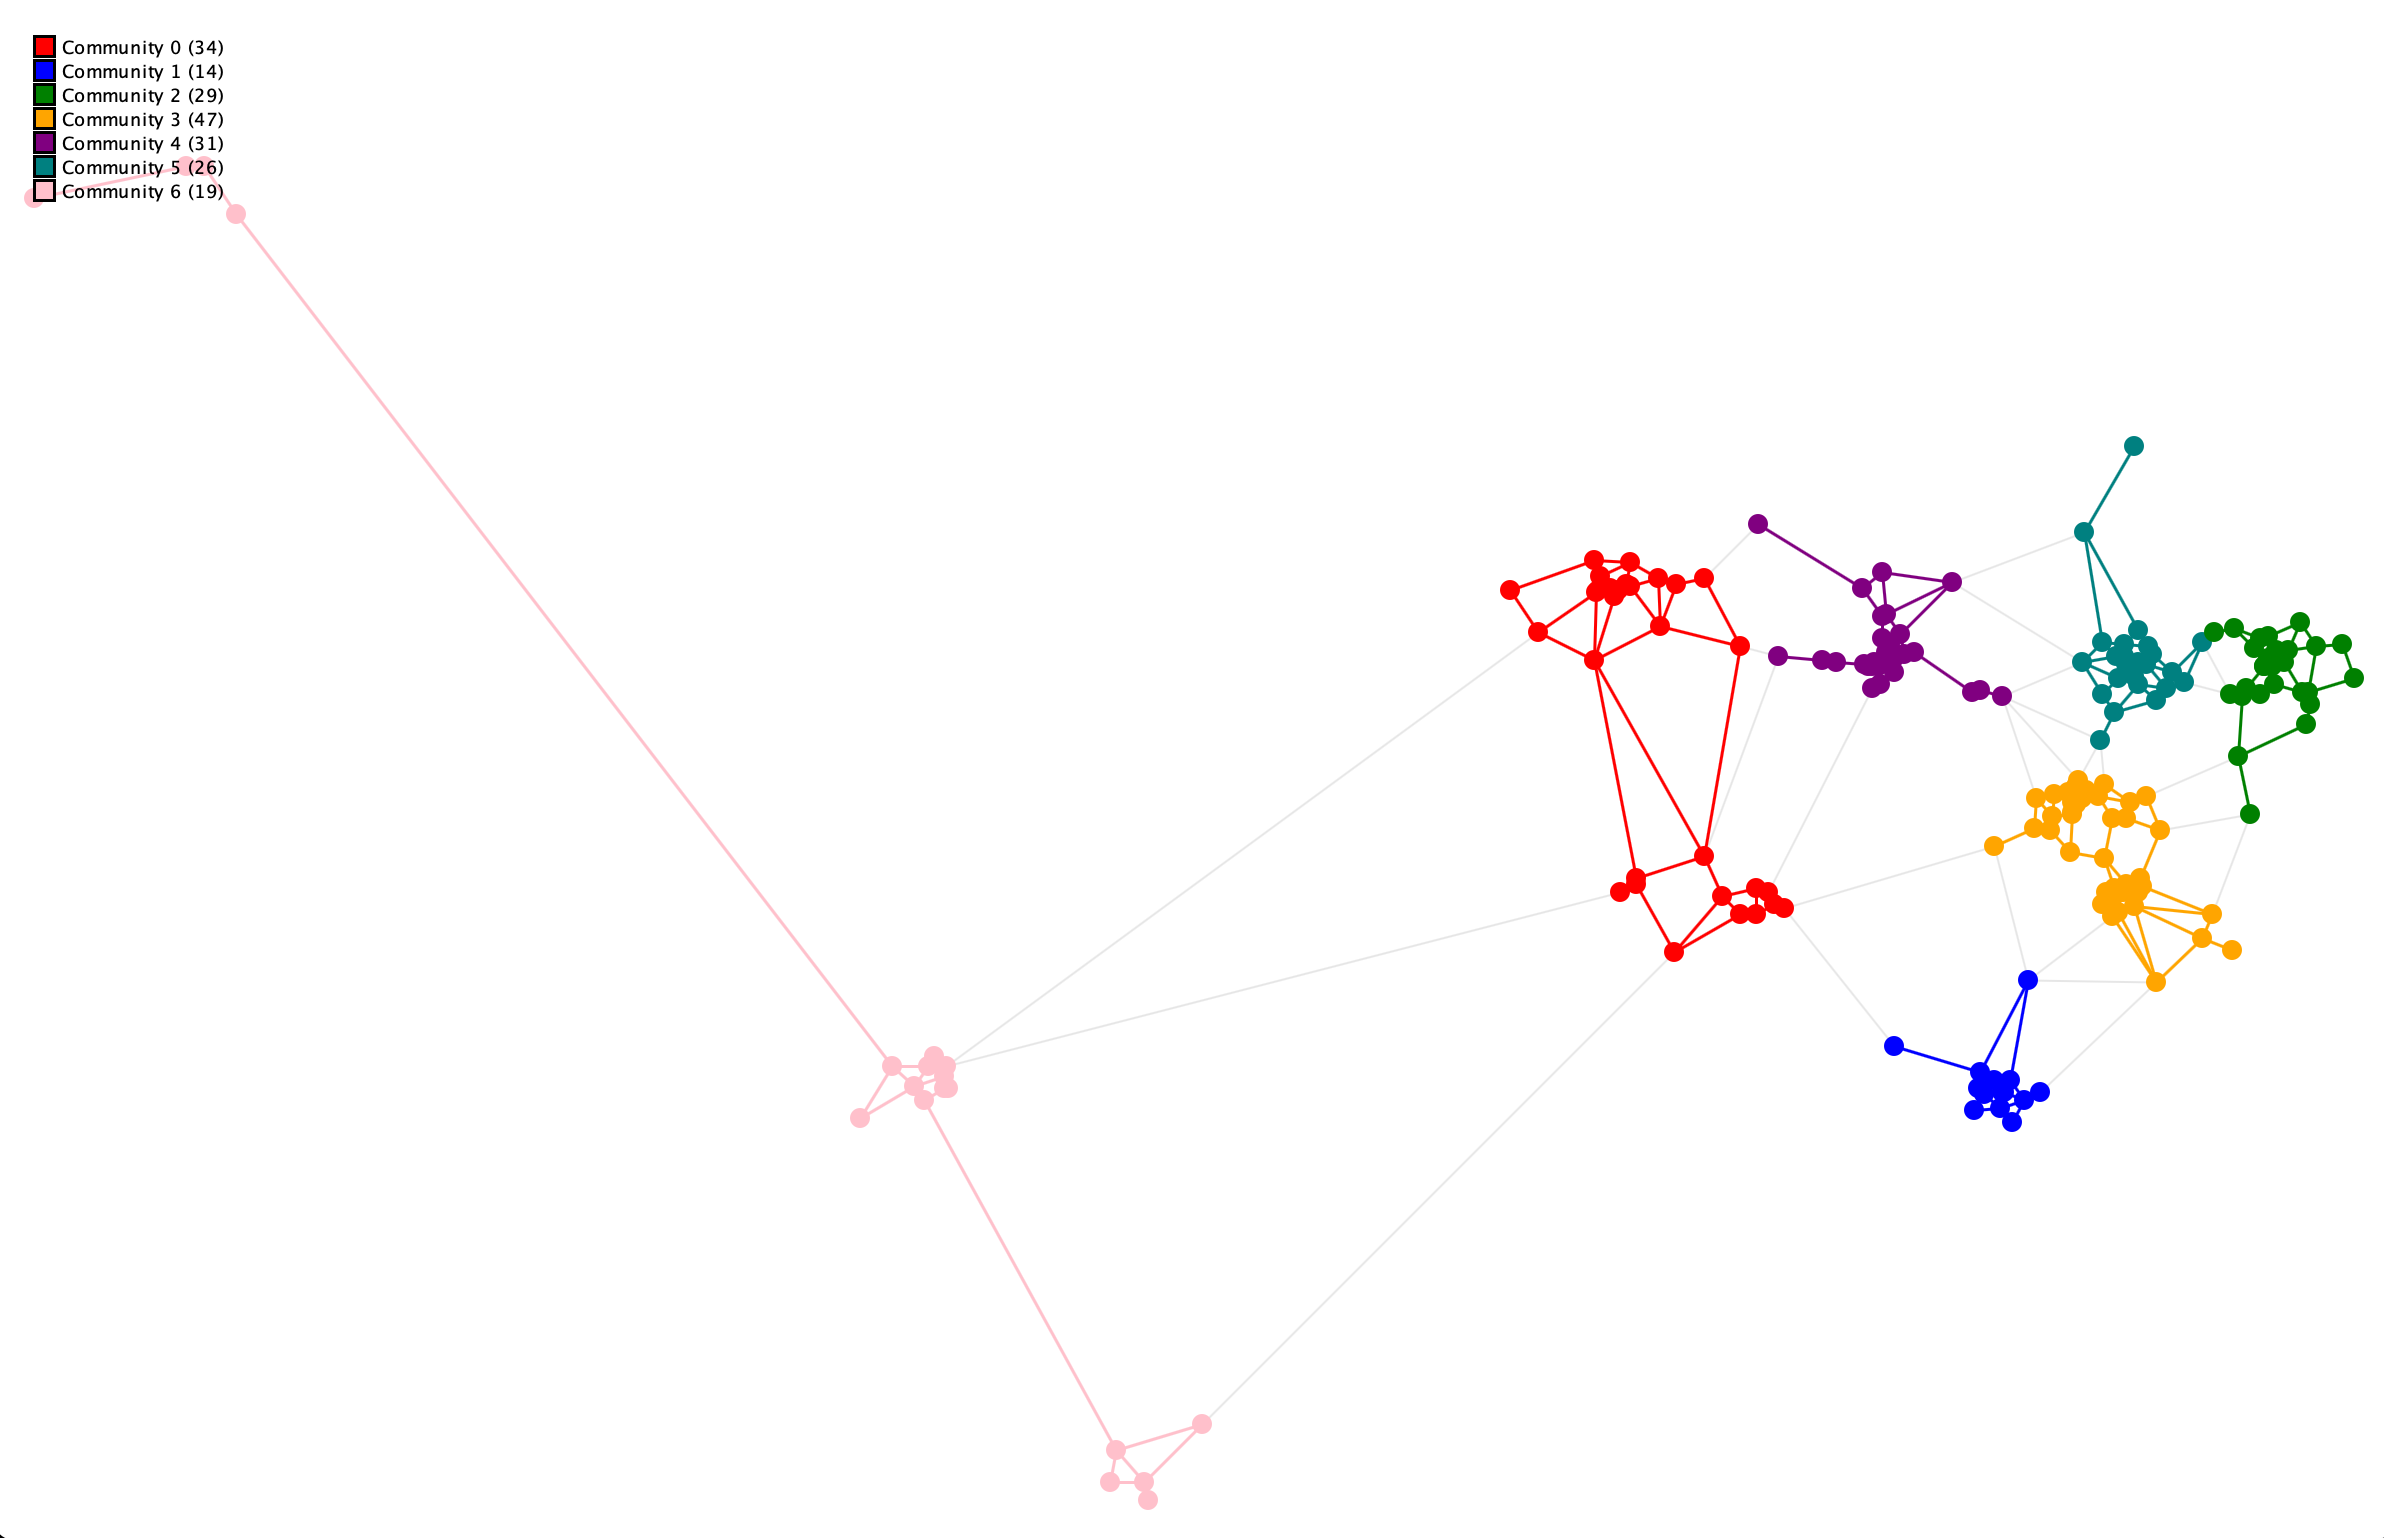
\includegraphics[width=0.7\textwidth]{./img/Leiden_Gabriel}
\vspace{0.5cm}

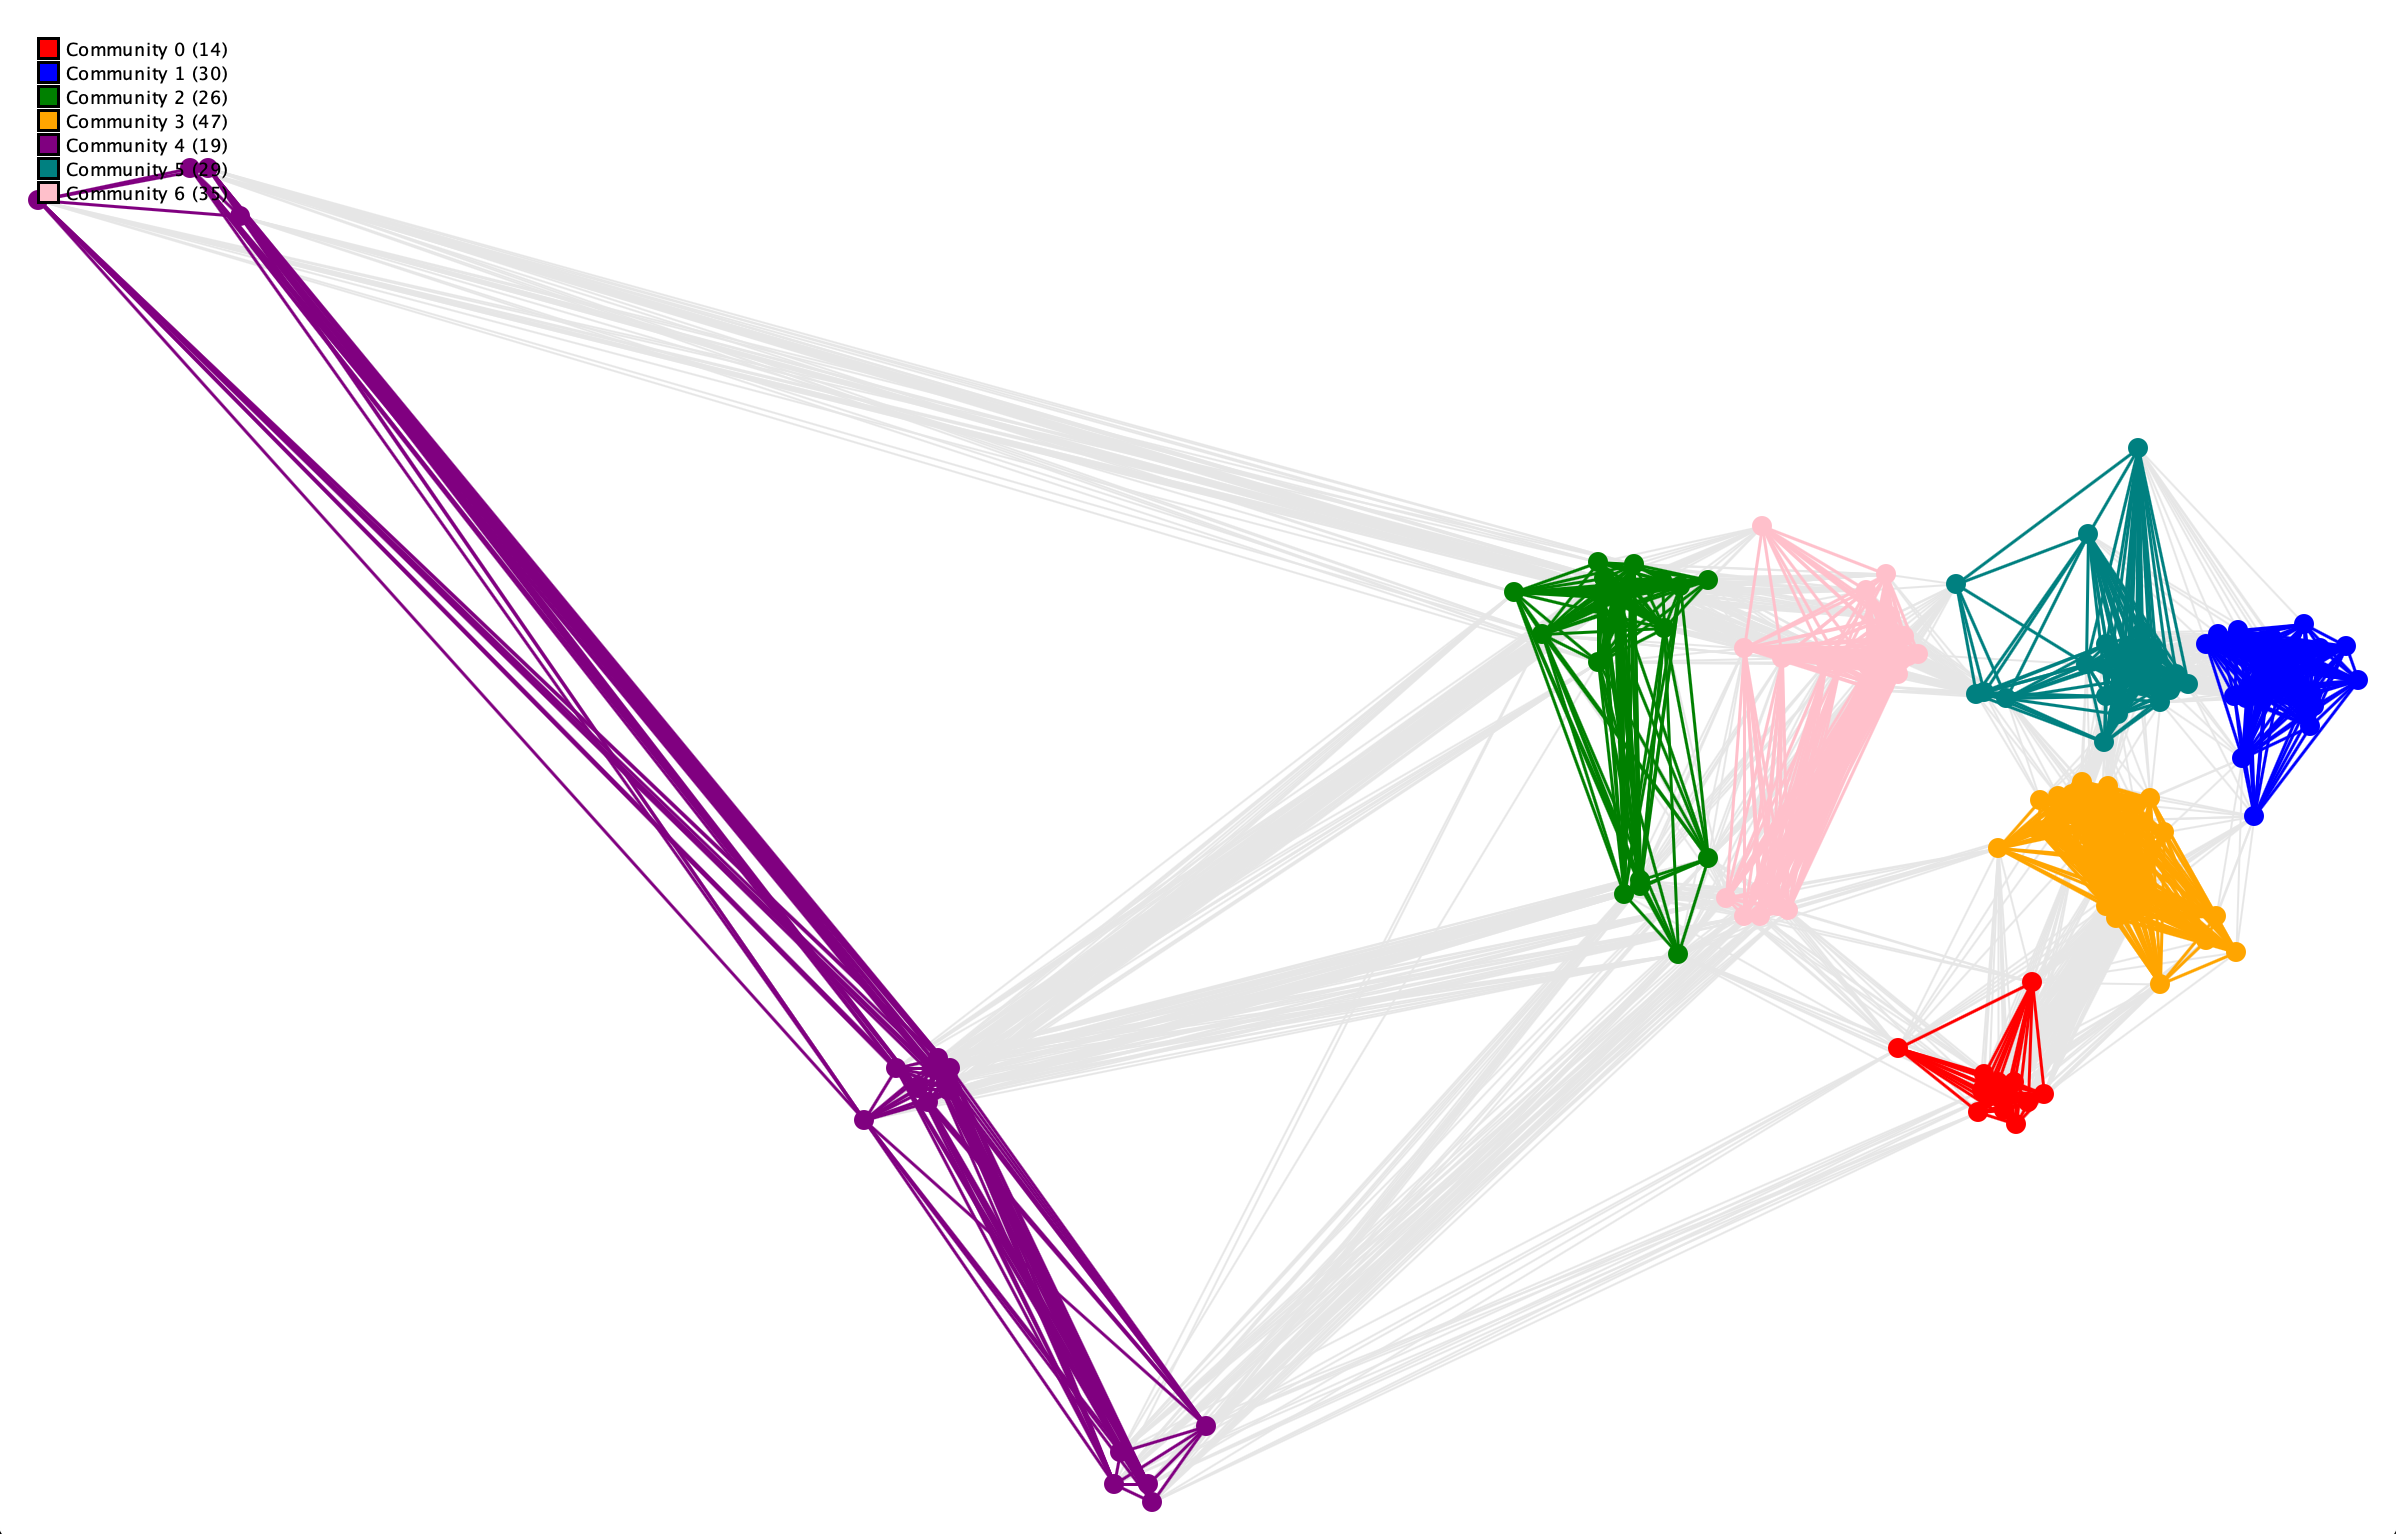
\includegraphics[width=0.7\textwidth]{./img/Leiden_K}

\caption{Leiden algorithm applied to different sparse graph representations (top: Delaunay, middle: Gabriel, bottom: K-Nearest) with 200 student locations.}
\label{fig:leiden_clustering}
\end{figure}

Figure \ref{fig:leiden_clustering} shows the clustering results of our Leiden algorithm implementation across three graph types. On Delaunay triangulation, Leiden identifies geographically coherent communities with balanced sizes; on Gabriel graph, the algorithm forms more compact clusters with clear boundaries; on K-Nearest Neighbors (k=30), Leiden captures local density variations, creating more clusters in densely populated areas and larger clusters in sparse regions.

The Leiden algorithm demonstrates effectiveness at identifying meaningful communities in the transportation network. The visualization reveals how our implementation produces clusters that strongly reflect the underlying graph topology while respecting geographical constraints. The smaller, more numerous clusters reflect the algorithm's emphasis on local connectivity and modularity optimization.

A distinctive characteristic of the Leiden implementation is its consistent performance across different sparse graph representations. This consistency stems from the algorithm's refinement phase, which ensures well-connected communities regardless of the initial graph structure. When examining the clusters formed on the Delaunay graph versus those on the Gabriel graph, we observe similar community sizes despite the different edge structures, demonstrating the algorithm's robustness.

The Leiden approach offers a balanced clustering solution for transportation planning, accommodating mixed vehicle fleets while maintaining reasonable geographic coherence within each cluster.

\subsubsection{Performing MVAGC on Sparse Graph Representations of IZTECH}
\label{subsubsec:mvagc_implementation}

Our MVAGC implementation was specifically adapted for geospatial data clustering. Rather than using random sampling for anchor points, we employed a geographically stratified selection process to ensure anchor points were well-distributed across Izmir's districts. This modification improved the algorithm's ability to create geographically coherent clusters. We configured the implementation with approximately 500 anchor points and employed higher-order filtering with a standardized cutoff threshold of 0.25 for ensuring smooth community boundaries.

\begin{figure}[htbp]
\centering
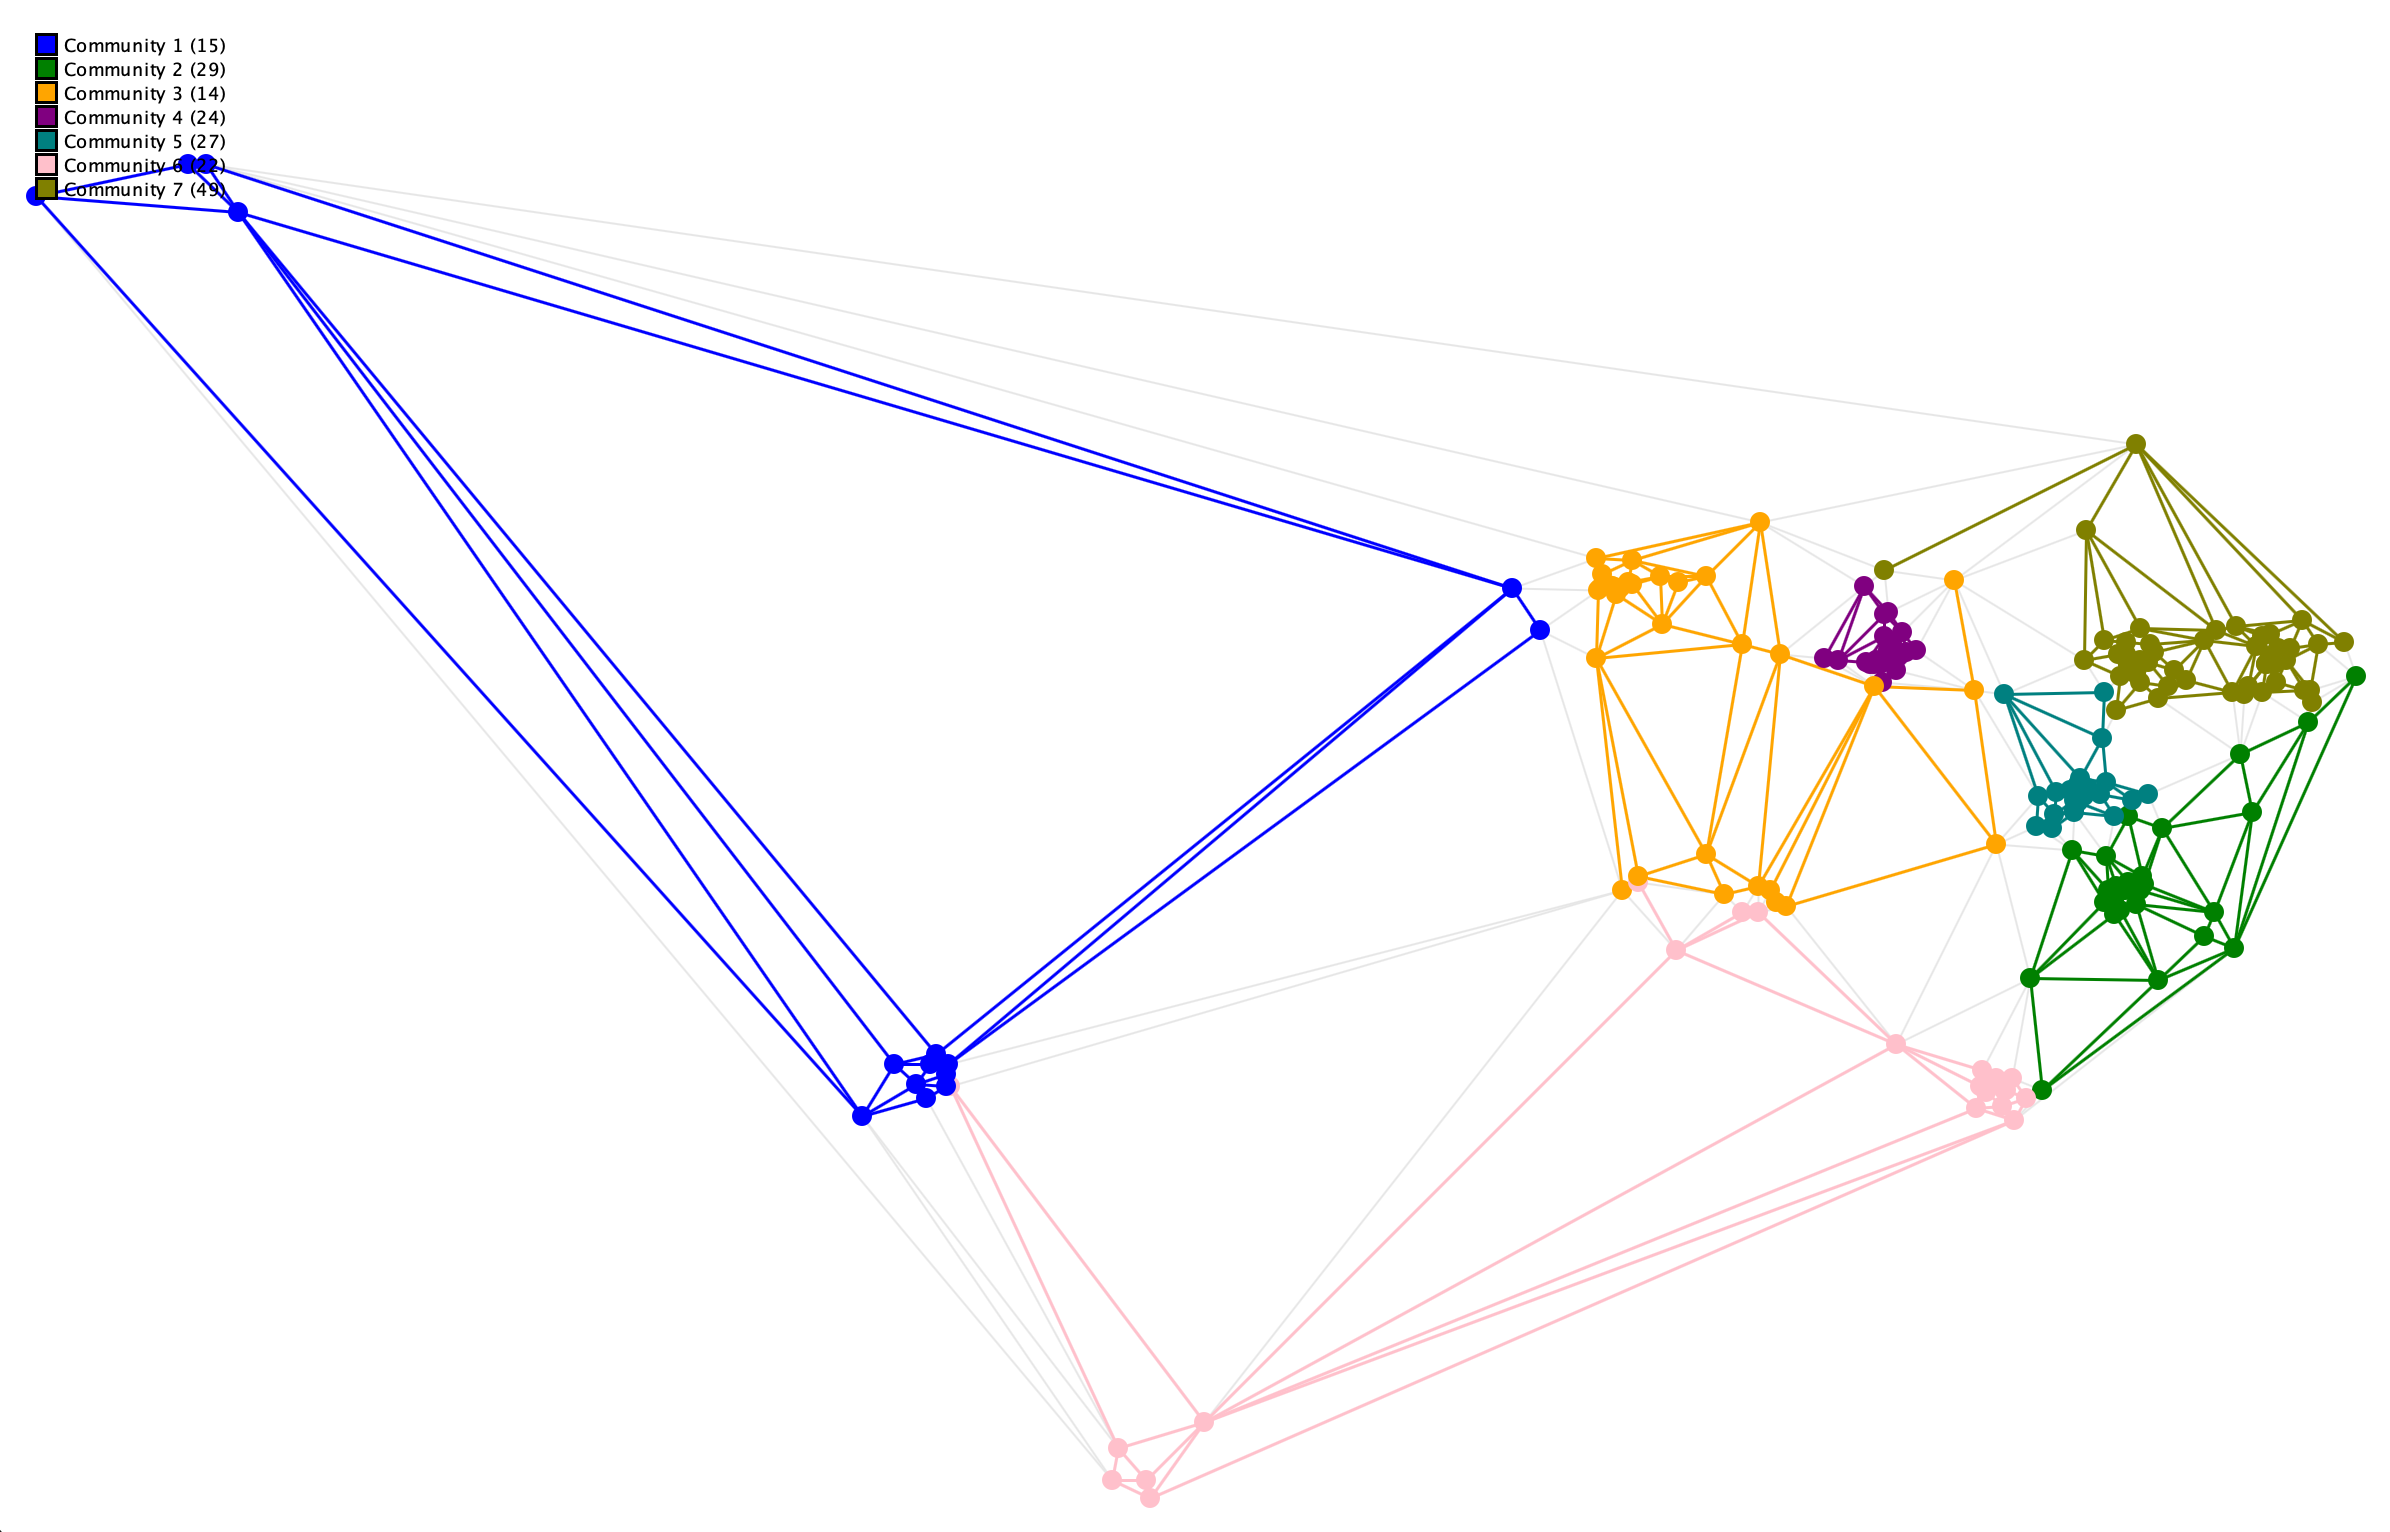
\includegraphics[width=0.7\textwidth]{./img/MVAGC_Delaunay}
\vspace{0.5cm}

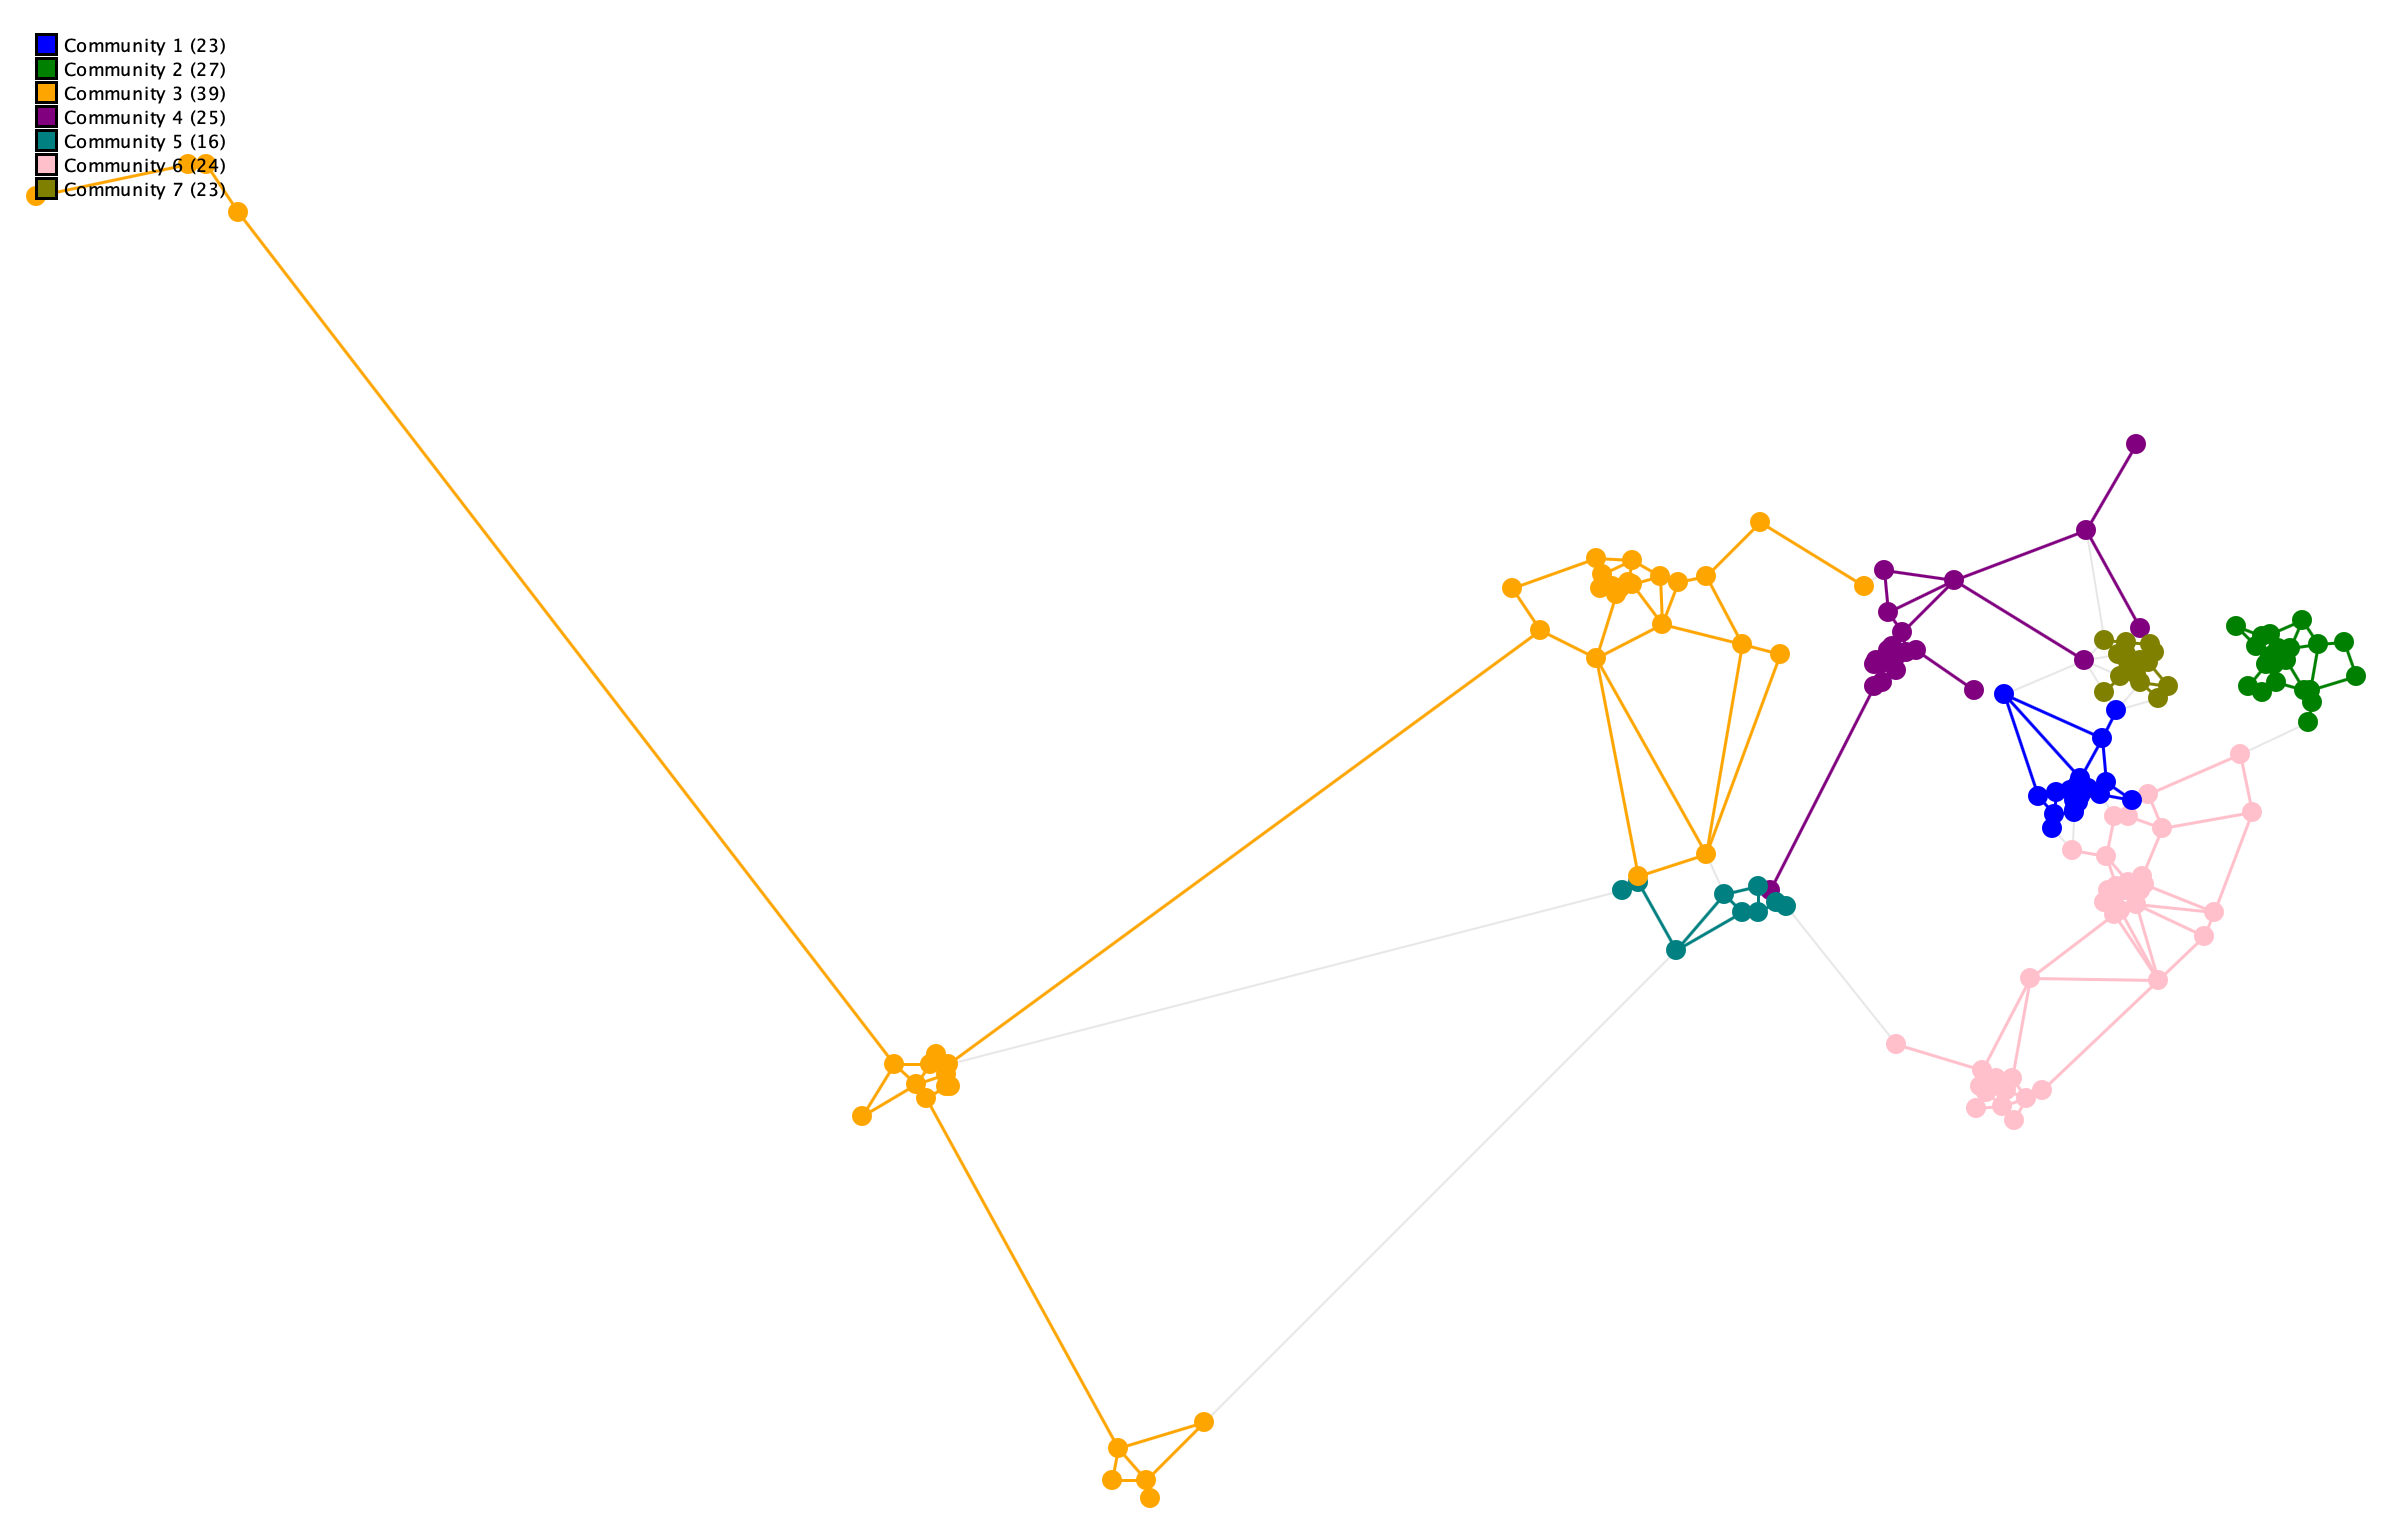
\includegraphics[width=0.7\textwidth]{./img/MVAGC_Gabriel}
\vspace{0.5cm}

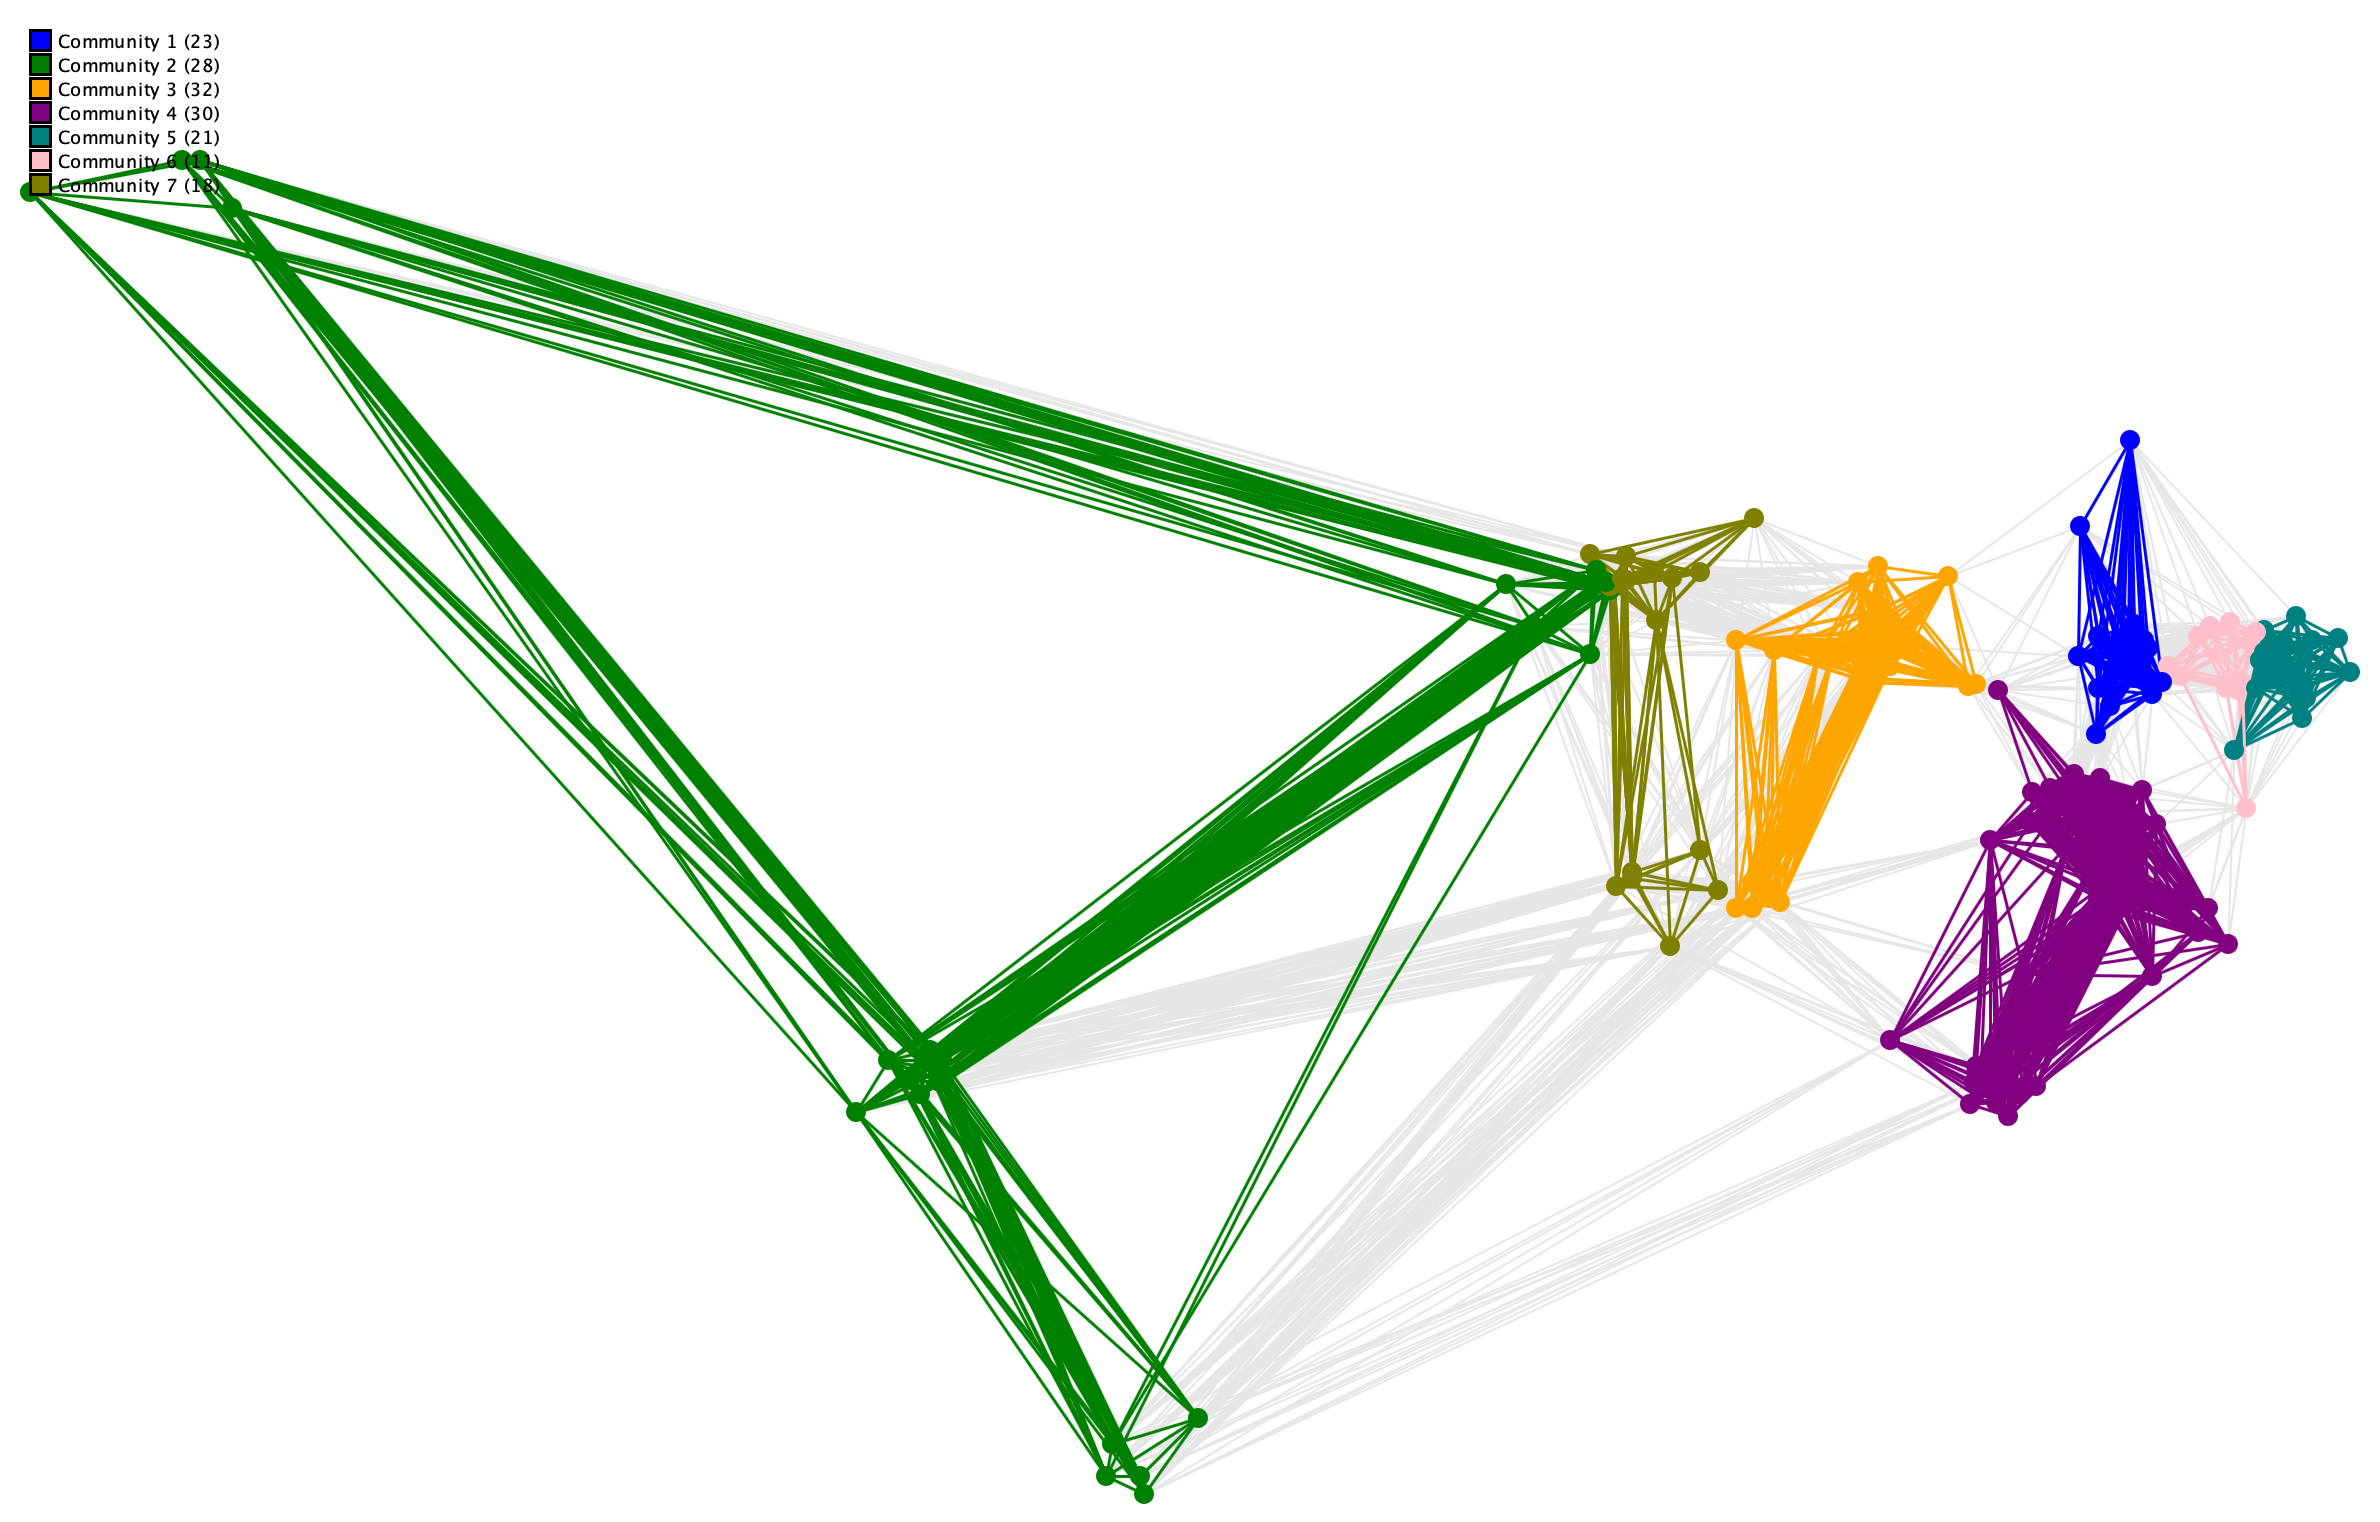
\includegraphics[width=0.7\textwidth]{./img/MVAGC_K}

\caption{MVAGC algorithm applied to different sparse graph representations (top: Delaunay, middle: Gabriel, bottom: K-Nearest) with 200 student locations.}
\label{fig:mvagc_clustering}
\end{figure}

Figure \ref{fig:mvagc_clustering} depicts the clustering patterns of the MVAGC algorithm on various graph representations. On Delaunay triangulation, MVAGC creates numerous small, evenly distributed clusters that follow natural geographic contours; on Gabriel graph, the algorithm generates well-separated clusters with minimal fragmentation; on K-Nearest Neighbors (k=30), MVAGC demonstrates its highest performance, with clusters that naturally adapt to both dense urban areas and sparser suburban regions.

The distinctive clustering pattern produced by our MVAGC implementation shows a higher number of smaller clusters, reflecting the algorithm's anchor-based approach, which captures fine-grained community structures. This visualization demonstrates how MVAGC's multi-view perspective identifies different structural aspects of the transportation network that might be missed by single-view methods.

A notable characteristic of MVAGC is its sensitivity to the underlying graph structure, particularly with the K-Nearest Neighbors graph. This combination produces clusters that closely follow natural residential boundaries and traffic patterns. The method's ability to adapt to local density variations makes it particularly effective for areas with uneven student distribution across Izmir.

The MVAGC approach is well-suited for transportation planning scenarios that prioritize shorter, more efficient routes and have access to a larger number of smaller vehicles.

\subsubsection{Summary of Different Clustering Approaches}
\label{subsubsec:clustering_comparison}

\begin{table}[h]
\centering
\begin{tabular}{|l|c|c|c|}
\hline
\textbf{Graph + Algorithm} & \textbf{Avg. Cluster} & \textbf{Avg. Route} & \textbf{Avg. Fuel} \\
 & \textbf{Size} & \textbf{Length (km)} & \textbf{Cost (TL)} \\
\hline
Delaunay + Spectral & 19.8 & 17.5 & 323.4 \\
\hline
Gabriel + Spectral & 20.5 & 23.4 & 434.5 \\
\hline
KNN + Spectral & 20.7 & 20.9 & 389.3 \\
\hline
Delaunay + Leiden & 14.5 & 13.7 & 227.6 \\
\hline
Gabriel + Leiden & 16.4 & 14.0 & 235.8 \\
\hline
KNN + Leiden & 15.8 & 14.1 & 244.4 \\
\hline
Delaunay + MVAGC & 12.7 & 16.6 & 263.9 \\
\hline
Gabriel + MVAGC & 14.5 & 15.8 & 265.8 \\
\hline
KNN + MVAGC & 14.3 & 12.4 & 205.5 \\
\hline
\end{tabular}
\caption{Characteristic parameters of different combinations of graph construction and clustering algorithms}
\label{tab:sparse_clustering_comparison}
\end{table}

Table \ref{tab:sparse_clustering_comparison} provides an overview of the characteristic parameters observed when applying the different clustering approaches to sparse graph representations. These parameters illustrate the inherent tendencies of each method rather than final performance metrics, which are analyzed in Chapter~\ref{ch:experiments}.

Among the graph construction methods, the K-Nearest Neighbors approach creates network structures that balance edge sparsity with node connectivity, particularly beneficial for MVAGC. The Gabriel graph representation creates well-defined spatial partitions but can lead to more dispersed clusters when combined with Spectral clustering due to the removal of certain edges present in the Delaunay triangulation.


\section{Shortest Path Computation for Route Optimization}
\label{sec:shortest_path}

After clustering the student locations into communities that represent potential bus routes, determining the optimal path through each cluster becomes essential for minimizing travel distance, time, and fuel consumption. We implemented Dijkstra's algorithm as the core method for computing optimal routes within each cluster.

This approach leverages the efficiency of Dijkstra's algorithm while addressing the practical challenges of route planning. Figure \ref{fig:route_optimization} illustrates a sample optimized route for a cluster.

\begin{figure}[!htbp]
\centering
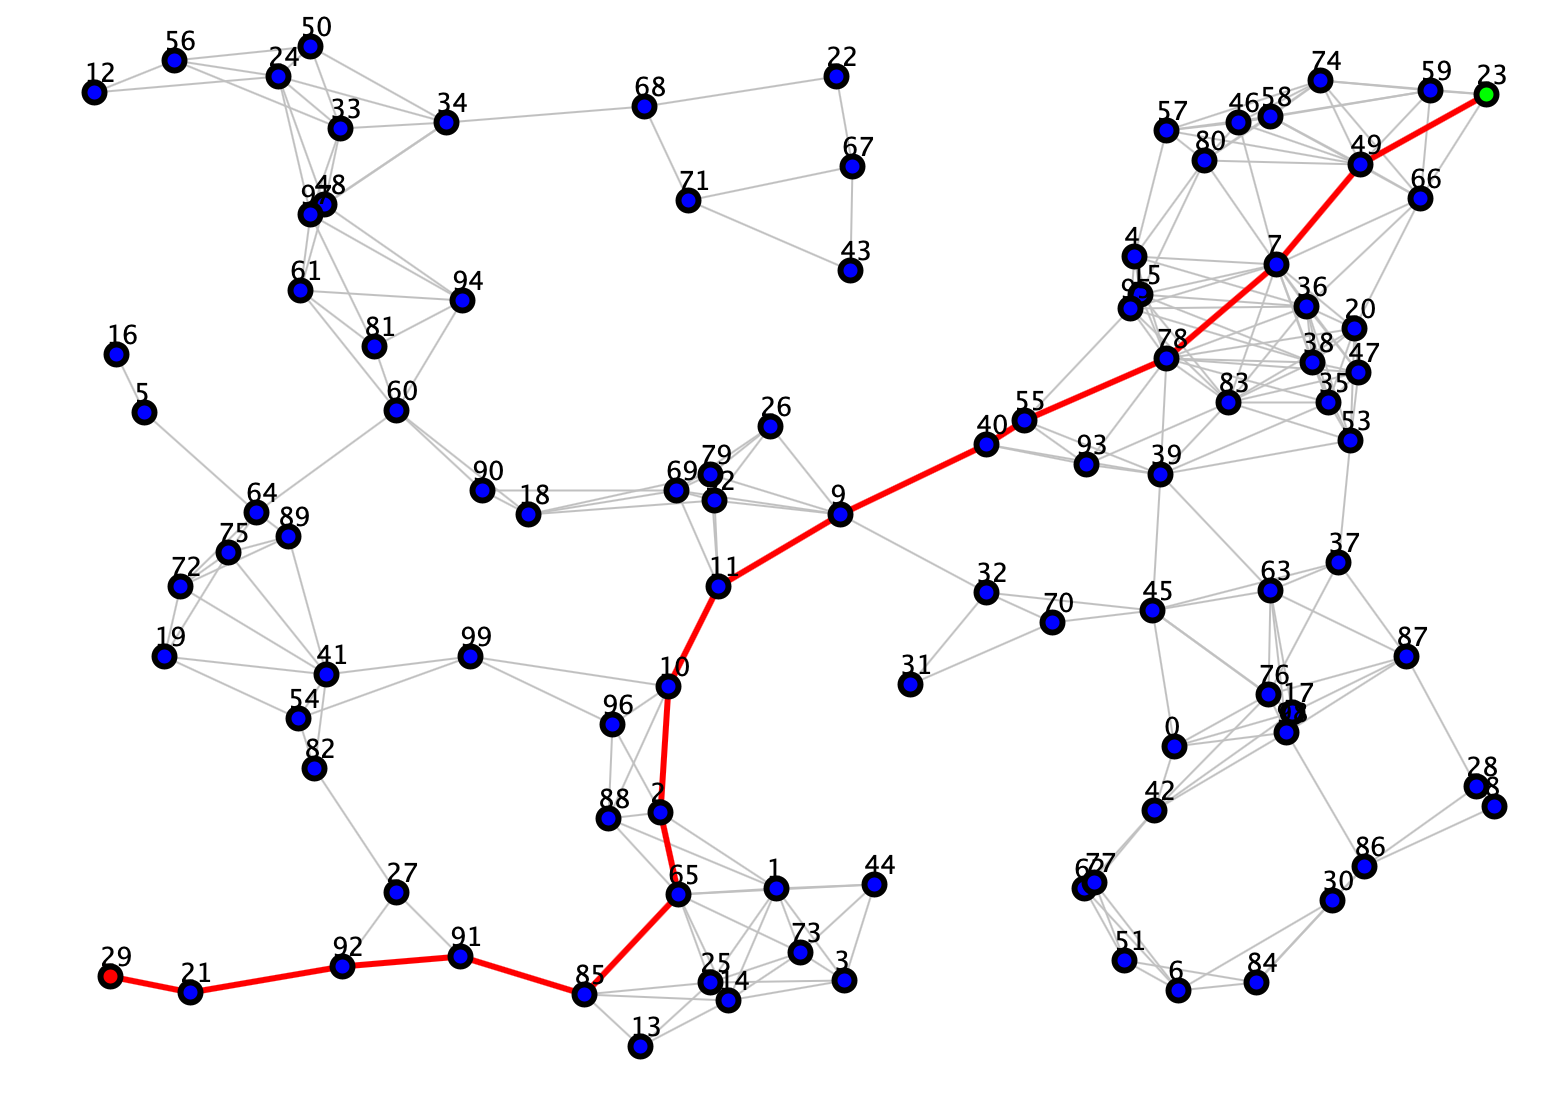
\includegraphics[width=0.8\textwidth]{img/shortest_path}
\caption{Example of an optimized route through a cluster of student locations. The red line represents the shortest path computed using Dijkstra's algorithm.}
\label{fig:route_optimization}
\end{figure}

\section{Robustness for Clustering Graph Representation of IZTECH}
\label{sec:robustness}

% Commenting out the example algorithm from the template
% \begin{algorithm}
% \begin{algorithmic}[1]
% \STATE generate random number $n \in [l, u]$
% \WHILE{$n \neq 42$}
% \IF{today is Tuesday}
% \STATE print(42)
% \ENDIF
% \ENDWHILE
% \RETURN best solution found so far
% \end{algorithmic}
% \caption{Basic Algorithm($l, u$)}
% \label{alg:example_alg}
% \end{algorithm}




\chapter{Experimental Evaluation}
\label{ch:experiments}

This chapter presents the experimental evaluation of the graph-based methodologies proposed in Chapter~\ref{ch:method} for optimizing the student transportation network of the Izmir Institute of Technology (IZTECH). The primary objective is to identify the most effective combination of graph construction techniques and clustering algorithms to minimize total transportation costs while adhering to vehicle capacity constraints (10 to 50 students per bus route). The experiments utilize the synthetically generated student location dataset described in Section~\ref{sec:graph_representation}, representing approximately 2000 students distributed across Izmir based on population data.

\section{Evaluation Metrics}
\label{sec:eval_metrics}

To quantitatively compare the different approaches, we employ the following evaluation metrics:
\begin{itemize}
    \item \textbf{Total Transportation Cost (TL):} Estimated based on the total distance traveled by all buses and fuel consumption rates. This is the primary optimization target.
    \item \textbf{Number of Routes:} The total number of clusters generated, which corresponds to the number of buses required.
    \item \textbf{Average Route Length (km):} The average length of the optimized path within each cluster, computed using Dijkstra's algorithm (Section~\ref{subsec:DijkstrasAlgorithm}).
    \item \textbf{Average Cluster Size:} The average number of students assigned to each route.
    \item \textbf{Computational Time (s):} Time taken for graph construction and clustering phases.
\end{itemize}

\section{Experiment 1: Impact of Graph Sparsity}
\label{sec:exp_sparsity}

We first analyze the impact of graph representation choice on the feasibility and outcome of the transportation network analysis. We compare the baseline Complete Graph (Section~\ref{subsec:complete_graph}) against the sparse representations: Delaunay Triangulation (Section~\ref{subsubsec:delaunay}), Gabriel Graph (Section~\ref{subsubsec:gabriel}), and K-Nearest Neighbors (KNN) graph with $k=30$ (Section~\ref{subsubsec:knn}).

Table~\ref{tab:graph_properties} summarizes the key properties of each graph constructed from the $|V| \approx 2000$ student locations. As expected, the sparse graphs significantly reduce the number of edges compared to the Complete Graph, making subsequent processing more computationally tractable.

\begin{table}[h]
\centering
% \caption{Properties of Different Graph Constructions for $|V| \approx 2000$ Student Locations}
\label{tab:graph_properties}
\begin{tabular}{lrrrr}
\toprule
Graph Type & $|V|$ & $|E|$ & Sparsity ($\frac{|E|}{|E_{complete}|}$) & Construction Time (s) \\
\midrule
Complete & $\approx 2000$ & $ 1,999,000$ & 1.0 & $ 43,200$ \\
Delaunay & $\approx 2000$ & $ 5,647$ & 0.0028 & 302 \\
Gabriel & $\approx 2000$ & $ 3,598$ & 0.0018 & 288 \\
KNN (k=30) & $\approx 2000$ & $ 39,899$ & 0.0200 & $ 1,350$ \\
\bottomrule
\end{tabular}
\caption{Properties of Different Graph Constructions for $|V| \approx 2000$ Student Locations.}
\end{table}

Clustering the Complete Graph (using the Leiden algorithm as described in Section~\ref{subsec:clustering_complete}) serves as a theoretical baseline. Notably, the construction time for the Complete Graph (43,200 seconds, or 12 hours) is orders of magnitude higher than for the sparse methods, further underscoring its impracticality for large datasets. However, as discussed in Section~\ref{subsubsec:minibus_solution}, clustering this graph often resulted in imbalanced clusters, with many routes having significantly fewer students than the maximum capacity. While the "minibus solution" showed potential cost savings by using smaller vehicles for smaller clusters, this is not currently feasible with IZTECH's fleet. This highlights the need for sparse graph representations that might naturally lead to more balanced clusters suitable for standard buses. Table~\ref{tab:complete_graph_clustering} shows the baseline results from clustering the complete graph. Detailed route information can be found in Appendix~\ref{sec:appendix_detailed_results}, Table~\ref{tab:appendix_leiden_complete}.

\begin{table}[h]
\centering
% \caption{Baseline Clustering Results on the Complete Graph (Leiden Algorithm)}
\label{tab:complete_graph_clustering}
\begin{tabular}{lr}
\toprule
Metric & Value \\
\midrule
Total Cost (TL) & 123,882.96 \\
Number of Routes & 68 \\
Average Route Length (km) & 12.15 \\
Average Cluster Size & 29.18 \\
Computation Time (s) & 122 \\
\bottomrule
\end{tabular}
\caption{Baseline Clustering Results on the Complete Graph (Leiden Algorithm, Only Buses).}
\end{table}

The high computational cost and tendency towards imbalanced clusters motivate the evaluation of clustering algorithms on the sparse graph representations.

\section{Experiment 2: Comparison of Clustering Algorithms on Sparse Graphs}
\label{sec:exp_clustering}

We evaluated three distinct clustering algorithms, detailed in Section~\ref{se:GraphBasedClusterings}, on the sparse graph representations: Spectral Clustering (Section~\ref{subsec:SpectralClustering}), Leiden Algorithm (Section~\ref{subsec:LeidenAlgorithm}), and Multi-view Anchor Graph-based Clustering (MVAGC) (Section~\ref{subsec:MVAGC}). Each algorithm was configured as described in Section~\ref{subsec:clustering_sparse}, including post-processing steps to enforce the 10-50 student capacity constraints.

Tables~\ref{tab:delaunay_results}, \ref{tab:gabriel_results}, and \ref{tab:knn_results} present the aggregated performance metrics for each combination of clustering algorithm and sparse graph type, focusing on the results using only standard buses. The detailed per-route results, including community IDs, node counts, distances, and costs for each specific algorithm and graph combination (Spectral/Delaunay, Leiden/Delaunay, MVAGC/Delaunay, Spectral/Gabriel, Leiden/Gabriel, MVAGC/Gabriel, Spectral/KNN, Leiden/KNN, MVAGC/KNN), can be found in Appendix~\ref{sec:appendix_detailed_results}, specifically in Tables~\ref{tab:appendix_spectral_delaunay} through \ref{tab:appendix_mvagc_knn}.

% Table for Delaunay Results
\begin{table}[h]
\centering
% \caption{Performance Comparison on Delaunay Graph}
\label{tab:delaunay_results}
\begin{tabular}{lrrr}
\toprule
Metric & Spectral & Leiden & MVAGC \\
\midrule
Total Cost (TL) & 133,245.21 & 121,145.10 & 143,428.94 \\
Number of Routes & 73 & 66 & 76 \\
Average Route Length (km) & 12.34 & 12.89 & 15.67 \\
Average Cluster Size & 26.90 & 29.76 & 25.84 \\
Computation Time (s) & 42 & 12 & 45 \\
\bottomrule
\end{tabular}
\caption{Performance Comparison of Clustering Algorithms on the Delaunay Graph (Only Buses).}
\end{table}

% Table for Gabriel Results
\begin{table}[h]
\centering
% \caption{Performance Comparison on Gabriel Graph}
\label{tab:gabriel_results}
\begin{tabular}{lrrr}
\toprule
Metric & Spectral & Leiden & MVAGC \\
\midrule
Total Cost (TL) & 127,944.52 & 110,364.09 & 135,654.57 \\
Number of Routes & 69 & 60 & 74 \\
Average Route Length (km) & 13.90 & 13.10 & 12.76 \\
Average Cluster Size & 28.38 & 32.63 & 26.46 \\
Computation Time (s) & 40 & 11 & 41 \\
\bottomrule
\end{tabular}
\caption{Performance Comparison of Clustering Algorithms on the Gabriel Graph (Only Buses).}
\end{table}

% Table for KNN Results
\begin{table}[h]
\centering
% \caption{Performance Comparison on KNN Graph (k=30)}
\label{tab:knn_results}
\begin{tabular}{lrrr}
\toprule
Metric & Spectral & Leiden & MVAGC \\
\midrule
Total Cost (TL) & 123,481.86 & 118,522.79 & 124,112.47 \\
Number of Routes & 68 & 65 & 69 \\
Average Route Length (km) & 11.40 & 12.24 & 10.91 \\
Average Cluster Size & 29.03 & 30.37 & 28.61 \\
Computation Time (s) & 75 & 22 & 78 \\
\bottomrule
\end{tabular}
\caption{Performance Comparison of Clustering Algorithms on the KNN Graph (k=30, Only Buses).}
\end{table}

Figures~\ref{fig:cost_comparison} and \ref{fig:routes_comparison} provide a visual summary of the total cost and number of routes across all combinations. Figure~\ref{fig:best_clustering_viz} illustrates the geographical distribution of clusters for the best performing combination identified (Leiden algorithm on Gabriel graph, based on the lowest total cost).

% Placeholder for Cost Comparison Bar Chart
\begin{figure}[h]
    \centering
    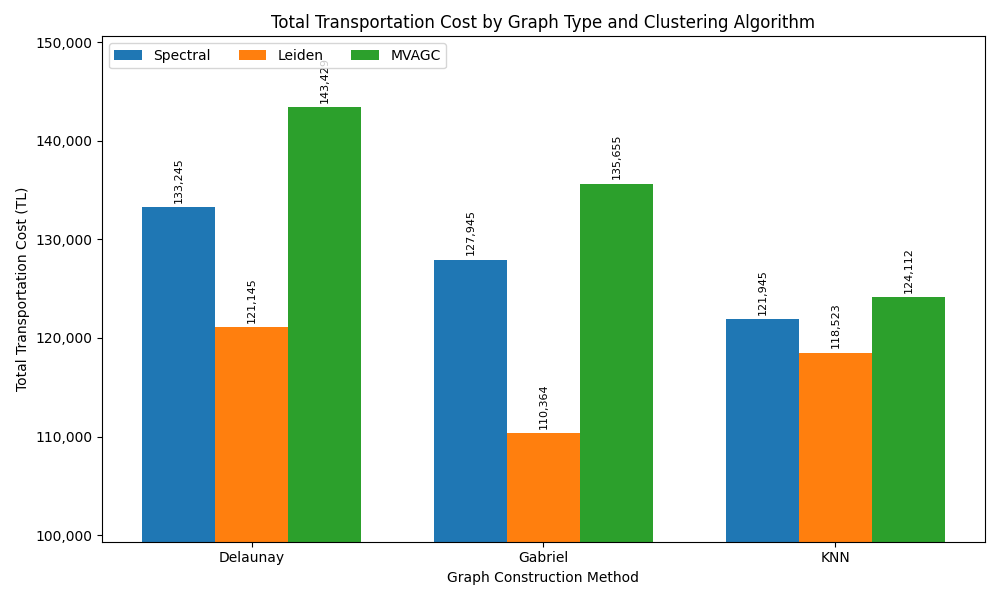
\includegraphics[width=0.8\textwidth]{img/cost_comparison}
    \fbox{Placeholder for Cost Comparison Bar Chart}
    \caption{Comparison of Total Transportation Cost across different graph types and clustering algorithms.}
    \label{fig:cost_comparison}
\end{figure}

% Placeholder for Routes Comparison Bar Chart
\begin{figure}[h]
    \centering
    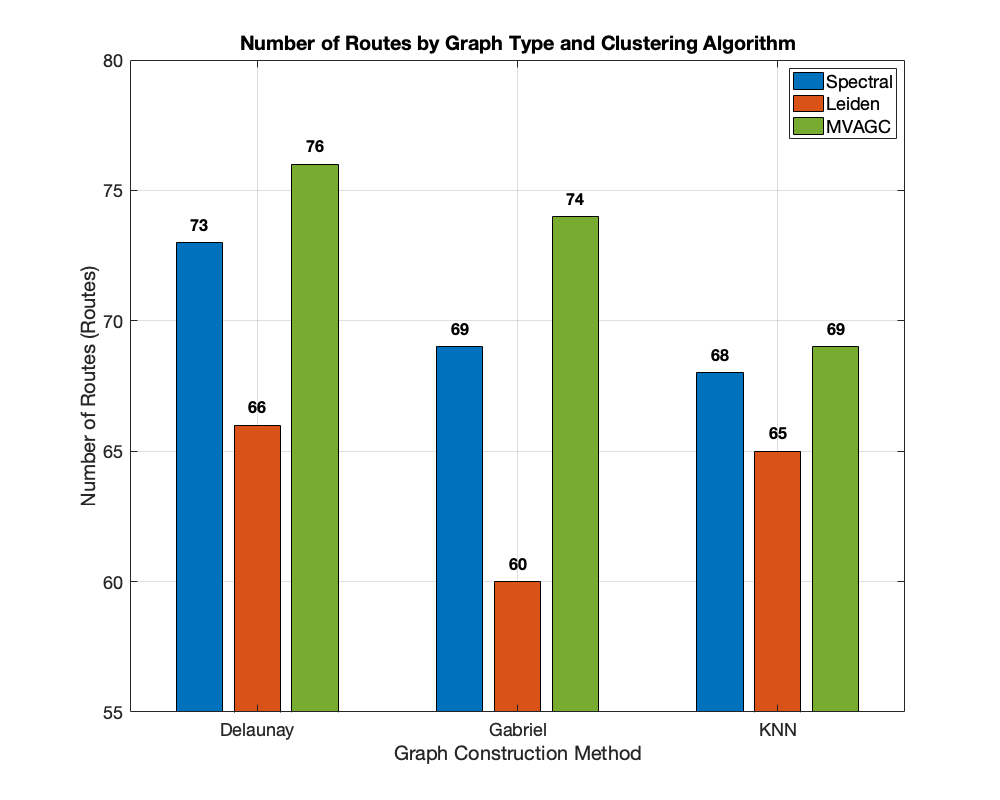
\includegraphics[width=0.8\textwidth]{img/route_count_comparison}
    \fbox{Placeholder for Route Count Bar Chart}
    \caption{Comparison of the Number of Routes Generated across different graph types and clustering algorithms.}
    \label{fig:routes_comparison}
\end{figure}

% Placeholder for Best Clustering Visualization
\begin{figure}[h]
    \centering
    % \includegraphics[width=0.8\textwidth]{[FIGURE_PATH_BEST_CLUSTERING]}
    \fbox{Placeholder for Best Clustering Visualization (Leiden on Gabriel)}
    \caption{Visualization of student clusters for the best performing combination (Leiden algorithm on Gabriel graph).}
    \label{fig:best_clustering_viz}
\end{figure}

The results indicate that the combination of the Gabriel graph and the Leiden algorithm yielded the lowest overall transportation cost (110,364.09 TL) and required the fewest buses (60). The Leiden/KNN combination was slightly more expensive but had a good average cluster size (30.37). The MVAGC/KNN combination yielded the shortest average routes (10.91 km) but required more buses (69) and had a higher cost (124,112.47 TL) than the top Leiden solutions. Spectral clustering generally resulted in higher costs and a comparable or higher number of routes than Leiden.

\section{Discussion}
\label{sec:discussion}

The experimental evaluation demonstrates the effectiveness of graph-based methods for optimizing the IZTECH student transportation network using only standard buses. Key findings include:

\begin{itemize}
    \item Sparse graph representations (Delaunay, Gabriel, KNN) are crucial for computational tractability and often lead to better routing solutions compared to the complete graph.
    \item The choice of both the sparse graph construction method and the clustering algorithm significantly impacts the final solution's cost, number of routes, and route characteristics.
    \item Based on our primary metric of minimizing total transportation cost, the combination of the \textbf{Gabriel graph} construction and the \textbf{Leiden algorithm} provided the most promising results, achieving a total cost of \textbf{110,364.09 TL} with \textbf{60} routes. This represents a cost saving of approximately 11% compared to the baseline Leiden/Complete graph result.
    \item Trade-offs exist: The Leiden/Gabriel combination had the lowest cost and fewest buses. The Leiden/KNN combination was slightly more expensive but had a good average cluster size (30.37). The MVAGC/KNN combination yielded the shortest average routes (10.91 km) but required more buses (69) and had a higher cost (124,112.47 TL) than the top Leiden solutions.
    \item The Leiden algorithm demonstrated strong performance, achieving the lowest cost on the Gabriel graph and the second-lowest cost on the KNN graph.
    \item All evaluated methods successfully produced routes adhering to the 10-50 student capacity constraints when applied to sparse graphs, unlike the baseline complete graph approach which tended towards imbalance (average size 29.18, but likely with wider variance not shown in summary).
\end{itemize}

These results suggest that adopting a \textbf{Gabriel graph representation combined with Leiden clustering} offers the strongest strategy for IZTECH to optimize its existing bus fleet usage, potentially leading to significant cost savings compared to less structured routing approaches or the baseline complete graph clustering. The Leiden/KNN combination presents a viable alternative if slightly higher costs are acceptable for potentially better balanced loads (average cluster size closer to 30). Further analysis could involve incorporating real road network distances instead of Euclidean distances and considering time-based constraints or traffic patterns.

% Remove the template figures and tables
% \begin{figure}[h] % do NOT use parameter h!
% \centerline{
% \subfigure[Title]{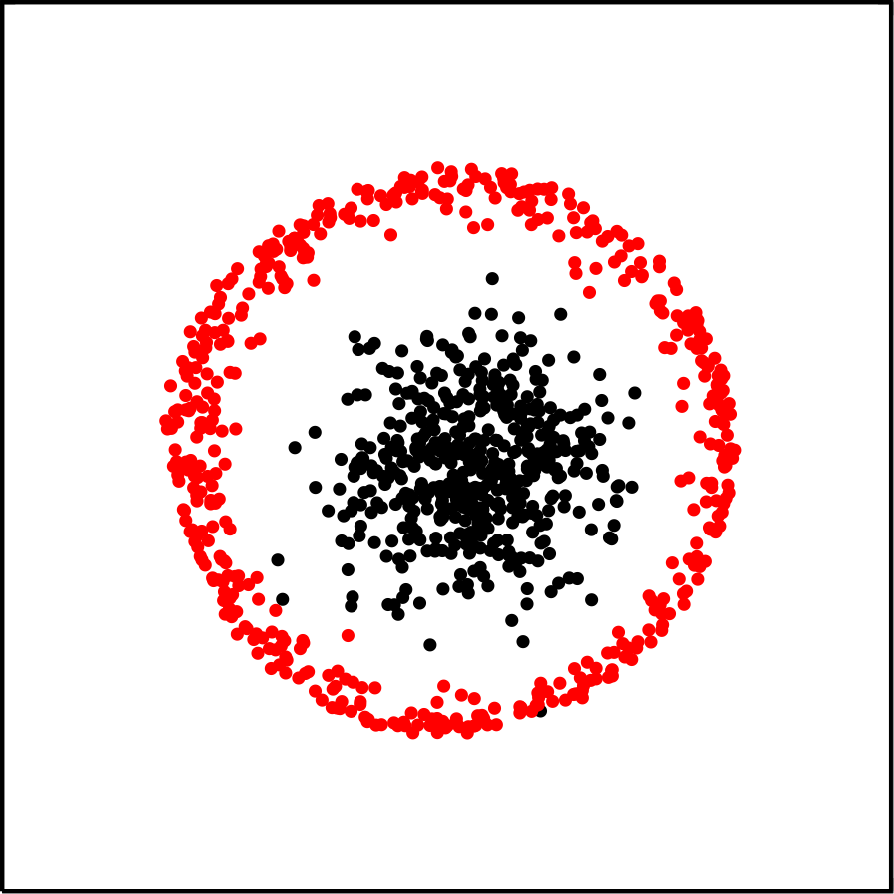
\includegraphics[width=1.5in]{img/subfig_a}}
% \subfigure[Title]{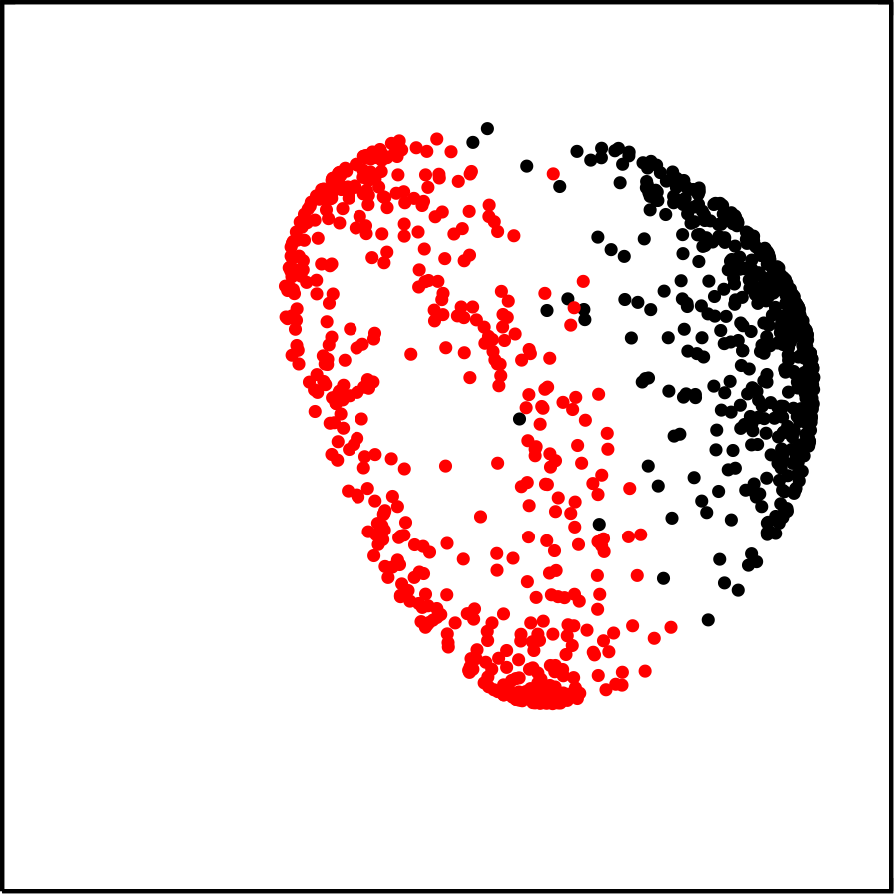
\includegraphics[width=1.5in]{img/subfig_b}}
% }
% \centerline{
% \subfigure[Title]{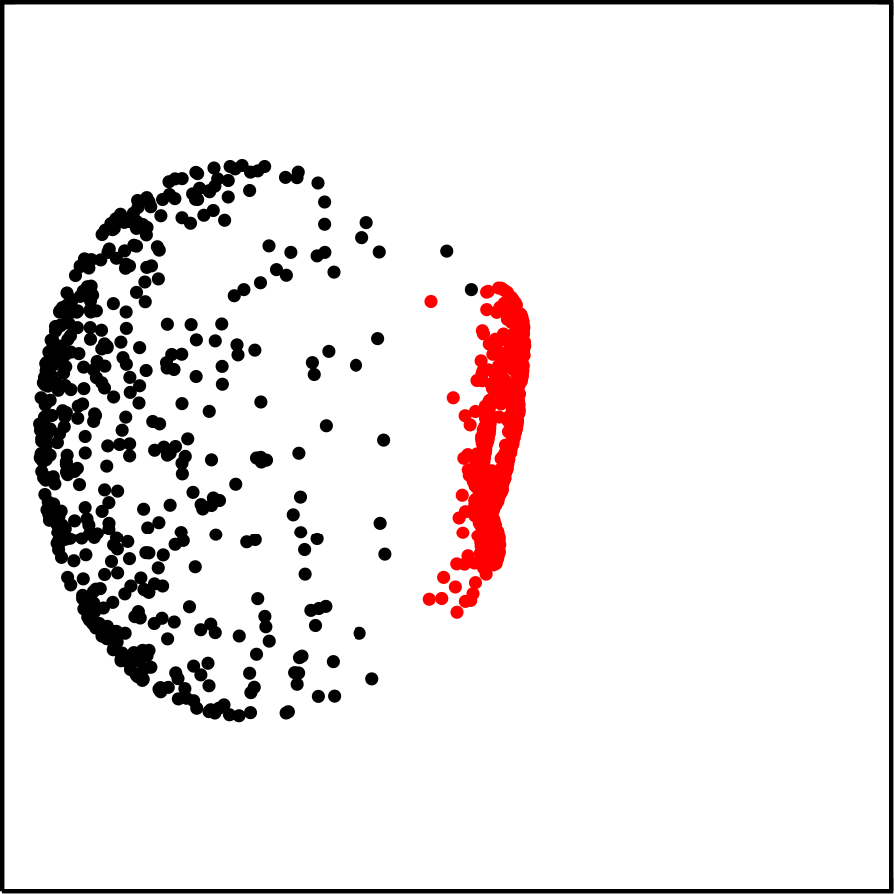
\includegraphics[width=1.5in]{img/subfig_c}}
% \subfigure[Title]{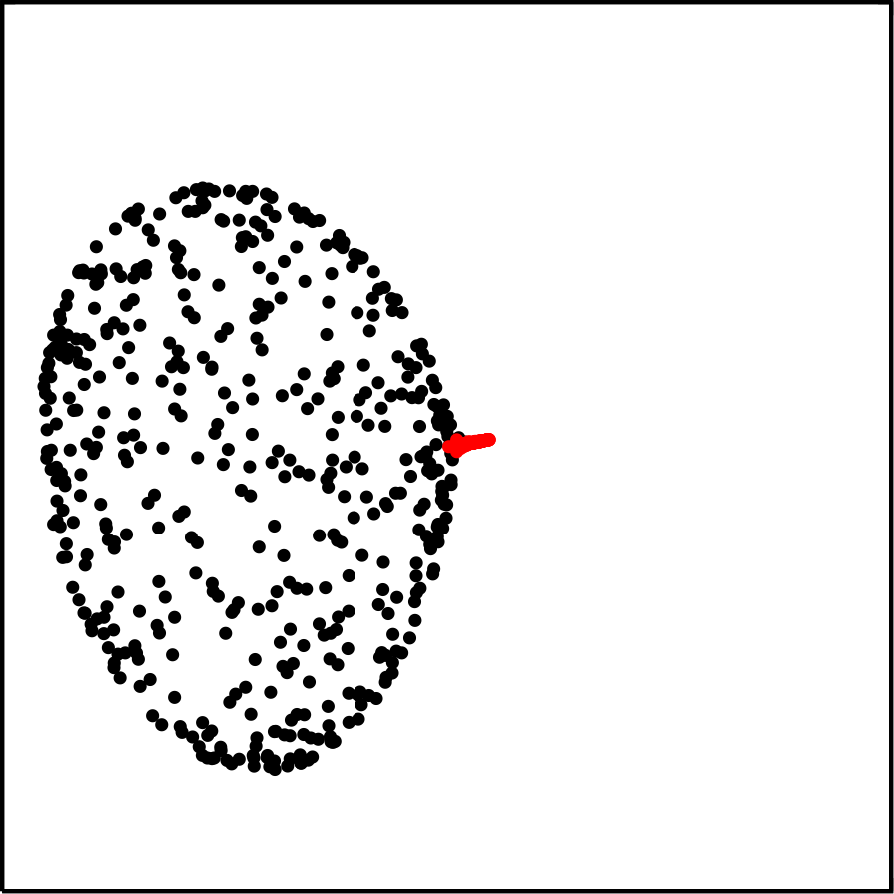
\includegraphics[width=1.5in]{img/subfig_d}}
% }
% \caption{Caption of the complete figure.}
% \label{fig:figure_1}
% \end{figure} 	
% \begin{figure}
% \centering
% 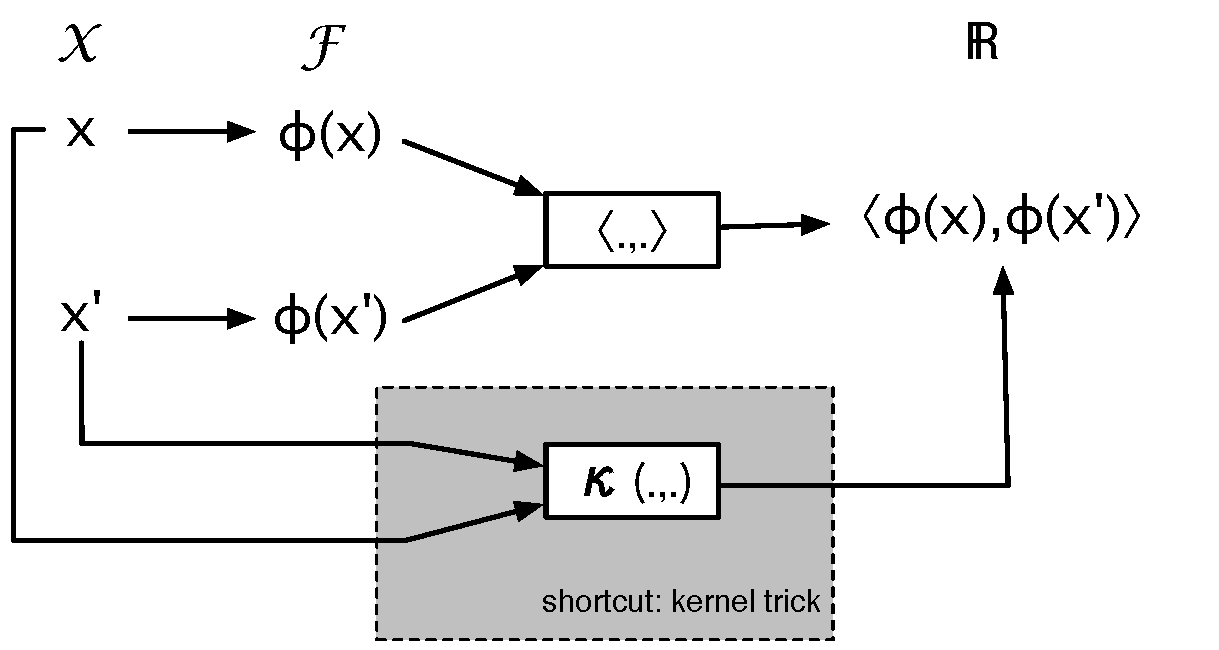
\includegraphics[scale=0.5]{img/figure}
% \caption{Caption of this figure.}
% \label{fig:figure_2}
% \end{figure}
% \begin{table}
% \centering
% {
% \begin{tabular}{ll}
% \addlinespace
% \toprule
% \addlinespace
% Lorem Ipsum \\
% \addlinespace
% \toprule
% \addlinespace
% diam & vero eos et accusam et justo \\
% justo & 10 (0, 1, 2, 3, 4, 5, 6, 7, 8, 9) \\
% aliquyam (q, w, t) &1,000, 500, 2,000\\
% voluptua & nonumy eirmod tempor (takimata sanctus)\\
% tempor & none \\
% gubergren & yes \\
% \bottomrule
% \end{tabular}
% }
% \caption{Basic characteristics of Lorem Ipsum.}
% \label{tab:table_1} 
% \end{table}
% \begin{table}
% \footnotesize{
% \centering{
% \begin{tabular}{@{}lp{1cm}p{1cm}p{1cm}p{1cm}@{}}
% \addlinespace
% \toprule
% \addlinespace
% & $k$-ta & \multicolumn{2}{c}{Lorem Ipsum Dolor}\\ 
% \addlinespace
% Ea Rebum & te & va & te\\ 
% \addlinespace
% \hline
% \addlinespace
% Gubergren           & 94.9 & 98.0 & 97.0~\ding{172}  \\
% \addlinespace
% Magna   & 66.9 & 72.4 & 68.6~\ding{182}  \\
% \addlinespace
% \bottomrule
% \end{tabular}
% }
% \caption{Lorem ipsum dolor sit amet, consetetur sadipscing elitr, sed diam nonumy eirmod tempor invidunt ut labore et dolore magna aliquyam erat, sed diam voluptua ($\alpha=0.05$): \ding{172}/\ding{182} At vero eos et accusam/justo, respectively.}
% \label{tab:table_2}
% }
% \end{table}




\chapter{Conclusions and Future Work}
\label{ch:conclusions}
Here come the conclusions and hints to future research activities. 



% endmatter
\begin{appendix}
\chapter{Appendix Title}
\label{appendix:appendix}

% Global settings for more compact tables in the appendix
\setlength{\tabcolsep}{3.5pt}  % Reduce column spacing
\renewcommand{\arraystretch}{0.85}  % Make table rows more compact

% Define a compact table environment for all tables in the appendix
\newenvironment{compacttable}
{\begingroup\footnotesize}
{\endgroup}

\section*{Note on Detailed Results Tables}
The detailed clustering results tables in this appendix present the per-route results for each algorithm. To conserve space, all tables use reduced font size and compact formatting.

\subsection*{Alternative Layout Options}
For better space utilization, consider one of these alternatives:

\begin{enumerate}
    \item \textbf{Multi-column layout}: Import the multicol package in main.tex and surround tables with:
    \begin{verbatim}
    \begin{multicols}{2}
    % Tables here
    \end{multicols}
    \end{verbatim}
    
    \item \textbf{Summary tables}: Instead of showing all community details, create summary tables showing statistics (min/max/avg distance, etc.) for each algorithm.
    
    \item \textbf{Digital appendix}: Move detailed tables to a digital appendix and only include key results in the printed thesis.
\end{enumerate}

\textbf{Example of Multi-Column Layout:} The following table demonstrates how results can be organized in a multi-column format to save space.

\begin{multicols}{2}
\begin{compacttable}
\begin{longtable}{@{}rrr@{}}
\caption{Example of Multi-Column Table Format}
\label{tab:example_multicol} \\
\toprule
\textbf{ID} & \textbf{Nodes} & \textbf{Cost} \\
\midrule
\endhead
\bottomrule
\endfoot
1 & 25 & 1820.55 \\
2 & 30 & 1956.23 \\
3 & 19 & 1754.88 \\
4 & 33 & 2014.76 \\
5 & 27 & 1865.40 \\
6 & 41 & 2103.92 \\
7 & 22 & 1788.35 \\
8 & 36 & 2055.19 \\
9 & 16 & 1722.50 \\
10 & 45 & 2188.67 \\
\end{longtable}
\end{compacttable}
\end{multicols}

\textbf{Example of Summary Table:} Instead of listing every community, a summary table can present key statistics:

\begin{compacttable}
\begin{tabularx}{\textwidth}{@{}lXXXXX@{}}
\toprule
\textbf{Algorithm} & \textbf{Graph} & \textbf{Clusters} & \textbf{Avg. Dist (km)} & \textbf{Min/Max Dist} & \textbf{Avg. Cost (TL)} \\
\midrule
Leiden & Complete & 72 & 13.7 & 1.5/50.2 & 1850.4 \\
Spectral & Delaunay & 74 & 10.3 & 1.2/30.3 & 1795.2 \\
Leiden & Delaunay & 71 & 14.1 & 4.6/46.7 & 1860.7 \\
MVAGC & Delaunay & 75 & 20.4 & 2.1/111.2 & 2055.6 \\
Spectral & Gabriel & 67 & 12.9 & 1.6/144.1 & 1836.2 \\
Leiden & Gabriel & 70 & 13.4 & 3.9/43.5 & 1850.8 \\
MVAGC & Gabriel & 72 & 15.3 & 0.8/41.9 & 1881.4 \\
Spectral & KNN & 67 & 11.8 & 2.4/29.9 & 1823.7 \\
Leiden & KNN & 74 & 13.5 & 3.2/38.4 & 1851.2 \\
MVAGC & KNN & 70 & 10.9 & 2.5/24.7 & 1804.5 \\
\bottomrule
\end{tabularx}
\end{compacttable}

Additional material can be placed here. Do not forget to refer to the appendix in the main part of your thesis.

\begin{algorithm}[H]
\caption{Leiden Algorithm}
\label{alg:leiden_appendix}
\begin{algorithmic}[1]
\Require Graph $G = (V, E)$, initial partition $P$ (optional)
\Ensure Final partition $P_{\text{final}}$ maximizing modularity $Q$

\State Initialize partition $P$ (e.g., each node in its own community).
\State Set \texttt{converged} = \texttt{false}.
\While{not \texttt{converged}}
    \State \textbf{Local Moving Phase}
    \State Set \texttt{moved\_nodes} = \texttt{true}.
    \While{\texttt{moved\_nodes}}
        \State Set \texttt{moved\_nodes} = \texttt{false}.
        \ForAll{node $i \in V$}
            \State Find neighboring community $C_j$ that maximizes $\Delta Q$ (Eq.~\eqref{eq:modularitygain}) for moving $i$ to $C_j$.
            \If{max $\Delta Q > 0$}
                \State Move node $i$ to community $C_j$.
                \State Update partition $P$.
                \State Set \texttt{moved\_nodes} = \texttt{true}.
            \EndIf
        \EndFor
    \EndWhile
    \State \textbf{Refinement Phase}
    \State Create refined partition $P'$ based on $P$.
    \ForAll{community $C \in P$}
        \State Partition $C$ into subcommunities locally (ensures well-connected).
        \State Add refined subcommunities of $C$ to $P'$.
    \EndFor
    \State Update $P = P'$.
    \State \textbf{Aggregation Phase}
    \If{no change in partition $P$ compared to previous iteration}
        \State Set \texttt{converged} = \texttt{true}.
    \Else
        \State Create aggregated graph $G'$ where each node represents a community in $P$.
        \State Set edge weights in $G'$ based on inter-community edge weights in $G$.
        \State Set $G = G'$ for the next iteration.
        \State Update node mappings to reflect aggregation.
    \EndIf
\EndWhile
\State Set $P_{\text{final}} = P$.
\end{algorithmic}
\end{algorithm}

\section{Detailed Clustering Results}
\label{sec:appendix_detailed_results}

This section provides the detailed per-route results for each combination of graph type and clustering algorithm evaluated in Chapter~\ref{ch:experiments}, considering only the standard bus scenario.

% --- Leiden Complete (Baseline) ---
\begin{compacttable}
\begin{longtable}{@{}rrrr@{}}
\caption{Detailed Results for Leiden Clustering on Complete Graph (Only Buses)}
\label{tab:appendix_leiden_complete} \\
\toprule
\textbf{Community ID} & \textbf{Node Count} & \textbf{Distance (km)} & \textbf{Total Cost (TL)} \\
\midrule
\endfirsthead
\caption[]{Continued} \\
\toprule
\textbf{Community ID} & \textbf{Node Count} & \textbf{Distance (km)} & \textbf{Total Cost (TL)} \\
\midrule
\endhead
\bottomrule
\endfoot
0 & 17 & 24.25 & 2046.61 \\
1 & 16 & 30.39 & 2160.80 \\
3 & 44 & 13.68 & 1850.22 \\
4 & 31 & 50.24 & 2529.77 \\
5 & 18 & 14.36 & 1862.95 \\
6 & 42 & 27.20 & 2101.53 \\
7 & 23 & 18.67 & 1943.00 \\
8 & 29 & 11.18 & 1803.77 \\
10 & 44 & 18.75 & 1944.57 \\
11 & 25 & 16.11 & 1895.36 \\
12 & 18 & 13.84 & 1853.15 \\
14 & 42 & 4.17 & 1673.47 \\
15 & 40 & 24.84 & 2057.59 \\
16 & 22 & 29.73 & 2148.50 \\
17 & 34 & 10.41 & 1789.56 \\
18 & 22 & 4.78 & 1684.88 \\
19 & 28 & 11.69 & 1813.17 \\
20 & 34 & 16.39 & 1900.55 \\
21 & 42 & 18.49 & 1939.69 \\
22 & 46 & 49.13 & 2509.18 \\
23 & 30 & 12.44 & 1827.15 \\
25 & 28 & 7.55 & 1736.23 \\
26 & 46 & 11.47 & 1809.21 \\
27 & 23 & 5.15 & 1691.69 \\
28 & 27 & 6.43 & 1715.54 \\
29 & 11 & 2.37 & 1640.03 \\
30 & 35 & 12.27 & 1824.09 \\
31 & 11 & 8.88 & 1760.98 \\
32 & 32 & 10.58 & 1792.56 \\
33 & 46 & 18.10 & 1932.40 \\
34 & 12 & 9.31 & 1768.99 \\
35 & 37 & 13.87 & 1853.73 \\
36 & 22 & 21.49 & 1995.47 \\
37 & 42 & 8.62 & 1756.16 \\
39 & 28 & 14.50 & 1865.48 \\
40 & 40 & 5.74 & 1702.71 \\
41 & 32 & 24.16 & 2045.01 \\
42 & 34 & 7.69 & 1738.97 \\
43 & 29 & 4.79 & 1684.98 \\
45 & 22 & 4.92 & 1687.40 \\
46 & 45 & 3.70 & 1664.78 \\
47 & 38 & 25.33 & 2066.73 \\
48 & 41 & 6.88 & 1723.78 \\
49 & 23 & 10.27 & 1786.83 \\
50 & 27 & 3.22 & 1655.86 \\
51 & 13 & 15.16 & 1877.69 \\
52 & 17 & 4.79 & 1685.06 \\
53 & 41 & 4.35 & 1676.83 \\
54 & 18 & 13.46 & 1846.10 \\
55 & 23 & 2.78 & 1647.60 \\
56 & 23 & 5.11 & 1690.96 \\
57 & 39 & 6.85 & 1723.28 \\
58 & 43 & 4.68 & 1683.00 \\
59 & 13 & 3.26 & 1656.61 \\
60 & 18 & 3.10 & 1653.70 \\
61 & 41 & 20.22 & 1971.88 \\
62 & 13 & 2.64 & 1645.00 \\
63 & 19 & 13.29 & 1842.98 \\
64 & 27 & 1.50 & 1623.86 \\
65 & 45 & 6.86 & 1723.53 \\
66 & 21 & 3.35 & 1658.24 \\
67 & 29 & 4.81 & 1685.32 \\
68 & 23 & 6.71 & 1720.77 \\
69 & 40 & 9.92 & 1780.37 \\
70 & 27 & 3.23 & 1656.06 \\
71 & 13 & 5.90 & 1705.67 \\
72 & 34 & 12.31 & 1824.77 \\
73 & 26 & 3.91 & 1668.58 \\
\end{longtable}
\end{compacttable}

% --- Spectral Delaunay ---
\begin{compacttable}
\begin{longtable}{@{}rrrr@{}}
\caption{Detailed Results for Spectral Clustering on Delaunay Graph (Only Buses, No Outlier Removal)}
\label{tab:appendix_spectral_delaunay} \\
\toprule
Community ID & Node Count & Distance (km) & Total Cost (TL) \\
\midrule
\endfirsthead
\caption[]{Continued} \\
\toprule
Community ID & Node Count & Distance (km) & Total Cost (TL) \\
\midrule
\endhead
\bottomrule
\endfoot
0 & 35 & 13.86 & 1853.56 \\
1 & 45 & 3.45 & 1660.17 \\
2 & 13 & 14.46 & 1864.71 \\
3 & 33 & 20.26 & 1972.54 \\
4 & 26 & 16.59 & 1904.29 \\
5 & 33 & 7.09 & 1727.84 \\
6 & 30 & 15.49 & 1883.94 \\
7 & 29 & 11.50 & 1809.70 \\
8 & 26 & 11.37 & 1807.34 \\
9 & 20 & 3.19 & 1655.36 \\
10 & 28 & 4.67 & 1682.75 \\
12 & 17 & 3.53 & 1661.60 \\
13 & 28 & 21.01 & 1986.45 \\
14 & 21 & 20.29 & 1973.11 \\
15 & 41 & 7.16 & 1729.07 \\
16 & 43 & 17.37 & 1918.78 \\
17 & 42 & 20.45 & 1976.11 \\
18 & 17 & 1.67 & 1627.11 \\
19 & 34 & 23.56 & 2033.78 \\
20 & 30 & 14.90 & 1872.97 \\
21 & 32 & 8.16 & 1747.56 \\
22 & 19 & 30.30 & 2159.06 \\
23 & 12 & 18.50 & 1939.84 \\
24 & 24 & 26.58 & 2090.09 \\
25 & 41 & 6.91 & 1724.43 \\
26 & 45 & 12.40 & 1826.54 \\
27 & 29 & 2.33 & 1639.28 \\
28 & 25 & 3.41 & 1659.45 \\
29 & 15 & 2.13 & 1635.65 \\
30 & 11 & 10.99 & 1800.30 \\
31 & 21 & 15.56 & 1885.26 \\
32 & 23 & 16.57 & 1904.01 \\
33 & 30 & 5.23 & 1693.13 \\
34 & 33 & 14.83 & 1871.56 \\
35 & 23 & 15.76 & 1888.86 \\
36 & 34 & 23.65 & 2035.51 \\
37 & 24 & 14.43 & 1864.23 \\
38 & 31 & 16.20 & 1897.13 \\
39 & 19 & 11.37 & 1807.35 \\
40 & 26 & 8.47 & 1753.48 \\
41 & 44 & 2.39 & 1640.44 \\
42 & 22 & 5.26 & 1693.71 \\
43 & 40 & 9.21 & 1767.15 \\
44 & 36 & 13.58 & 1848.38 \\
45 & 16 & 13.21 & 1841.59 \\
46 & 37 & 5.96 & 1706.71 \\
47 & 38 & 18.64 & 1942.39 \\
48 & 20 & 17.10 & 1913.89 \\
49 & 35 & 23.46 & 2032.00 \\
50 & 31 & 6.51 & 1716.99 \\
51 & 22 & 2.59 & 1644.08 \\
52 & 13 & 4.57 & 1680.89 \\
53 & 29 & 4.30 & 1675.99 \\
54 & 45 & 2.50 & 1642.48 \\
55 & 33 & 10.75 & 1795.78 \\
56 & 28 & 3.16 & 1654.67 \\
57 & 45 & 2.65 & 1645.23 \\
58 & 15 & 2.52 & 1642.74 \\
59 & 29 & 4.93 & 1687.53 \\
60 & 14 & 1.27 & 1619.65 \\
61 & 34 & 1.78 & 1629.05 \\
62 & 15 & 2.07 & 1634.39 \\
64 & 11 & 11.15 & 1803.21 \\
65 & 13 & 1.94 & 1632.03 \\
66 & 13 & 4.65 & 1682.39 \\
67 & 36 & 5.65 & 1701.02 \\
68 & 23 & 5.37 & 1695.72 \\
69 & 17 & 5.12 & 1691.15 \\
70 & 32 & 2.68 & 1645.80 \\
71 & 42 & 12.67 & 1831.47 \\
73 & 32 & 3.85 & 1667.53 \\
74 & 10 & 1.19 & 1618.03 \\
\end{longtable}
\end{compacttable}

% --- Leiden Delaunay ---
\begin{compacttable}
\begin{longtable}{@{}rrrr@{}}
\caption{Detailed Results for Leiden Clustering on Delaunay Graph (Only Buses, No Outlier Removal)}
\label{tab:appendix_leiden_delaunay} \\
\toprule
\textbf{Community ID} & \textbf{Node Count} & \textbf{Distance (km)} & \textbf{Total Cost (TL)} \\
\midrule
\endfirsthead
\caption[]{Continued} \\
\toprule
\textbf{Community ID} & \textbf{Node Count} & \textbf{Distance (km)} & \textbf{Total Cost (TL)} \\
\midrule
\endhead
\bottomrule
\endfoot
0 & 20 & 12.19 & 1822.62 \\
1 & 14 & 13.02 & 1837.97 \\
2 & 26 & 21.37 & 1993.17 \\
3 & 16 & 15.36 & 1881.50 \\
5 & 19 & 10.87 & 1798.05 \\
6 & 24 & 12.27 & 1824.02 \\
7 & 36 & 14.74 & 1869.87 \\
8 & 42 & 19.54 & 1959.18 \\
9 & 12 & 17.24 & 1916.37 \\
11 & 11 & 15.77 & 1889.07 \\
13 & 32 & 4.47 & 1679.13 \\
14 & 47 & 21.49 & 1995.48 \\
15 & 43 & 12.17 & 1822.17 \\
16 & 10 & 9.02 & 1763.60 \\
17 & 46 & 22.50 & 2014.08 \\
19 & 29 & 6.62 & 1719.11 \\
21 & 45 & 17.20 & 1915.73 \\
22 & 49 & 46.74 & 2464.66 \\
23 & 48 & 24.72 & 2055.50 \\
25 & 19 & 12.86 & 1835.06 \\
26 & 33 & 18.47 & 1939.23 \\
27 & 47 & 8.47 & 1753.41 \\
28 & 30 & 5.20 & 1692.72 \\
29 & 28 & 18.61 & 1941.93 \\
30 & 33 & 33.52 & 2219.06 \\
31 & 18 & 9.72 & 1776.66 \\
32 & 37 & 13.48 & 1846.46 \\
33 & 36 & 11.37 & 1807.37 \\
34 & 36 & 19.55 & 1959.34 \\
35 & 10 & 12.86 & 1835.06 \\
36 & 19 & 8.05 & 1745.59 \\
37 & 11 & 17.10 & 1913.84 \\
38 & 47 & 9.84 & 1778.89 \\
39 & 22 & 17.32 & 1917.90 \\
40 & 44 & 37.54 & 2293.65 \\
41 & 22 & 5.91 & 1705.91 \\
42 & 32 & 15.10 & 1876.64 \\
43 & 37 & 12.61 & 1830.35 \\
44 & 23 & 9.76 & 1777.39 \\
45 & 19 & 14.45 & 1864.60 \\
46 & 45 & 10.72 & 1795.15 \\
47 & 19 & 9.91 & 1780.24 \\
48 & 32 & 11.81 & 1815.57 \\
49 & 27 & 6.31 & 1713.29 \\
50 & 18 & 13.65 & 1849.69 \\
51 & 18 & 12.23 & 1823.34 \\
52 & 37 & 8.11 & 1746.65 \\
53 & 26 & 19.70 & 1962.08 \\
54 & 24 & 31.28 & 2177.28 \\
55 & 32 & 10.48 & 1790.69 \\
56 & 39 & 8.18 & 1748.11 \\
57 & 33 & 8.40 & 1752.19 \\
58 & 21 & 13.83 & 1853.06 \\
59 & 44 & 11.13 & 1802.83 \\
60 & 26 & 8.85 & 1760.39 \\
61 & 33 & 9.02 & 1763.72 \\
62 & 38 & 9.88 & 1779.68 \\
63 & 50 & 13.04 & 1838.37 \\
64 & 17 & 7.45 & 1734.41 \\
65 & 23 & 7.57 & 1736.70 \\
66 & 24 & 11.90 & 1817.10 \\
67 & 15 & 17.49 & 1921.01 \\
68 & 35 & 6.52 & 1717.11 \\
69 & 25 & 13.18 & 1841.00 \\
70 & 37 & 11.71 & 1813.70 \\
71 & 24 & 4.63 & 1682.01 \\
72 & 44 & 7.03 & 1726.58 \\
\end{longtable}
\end{compacttable}

% --- MVAGC Delaunay ---
\begin{compacttable}
\begin{longtable}{@{}rrrr@{}}
\caption{Detailed Results for MVAGC Clustering on Delaunay Graph (Only Buses, No Outlier Removal)}
\label{tab:appendix_mvagc_delaunay} \\
\toprule
\textbf{Community ID} & \textbf{Node Count} & \textbf{Distance (km)} & \textbf{Total Cost (TL)} \\
\midrule
\endfirsthead
\caption[]{Continued} \\
\toprule
\textbf{Community ID} & \textbf{Node Count} & \textbf{Distance (km)} & \textbf{Total Cost (TL)} \\
\midrule
\endhead
\bottomrule
\endfoot
0 & 24 & 22.42 & 2012.61 \\
2 & 36 & 24.17 & 2045.24 \\
3 & 37 & 41.62 & 2369.58 \\
4 & 25 & 11.08 & 1801.89 \\
6 & 22 & 33.05 & 2210.20 \\
9 & 17 & 17.50 & 1921.18 \\
10 & 31 & 34.06 & 2228.95 \\
19 & 14 & 58.13 & 2676.43 \\
27 & 16 & 40.99 & 2357.85 \\
33 & 18 & 19.10 & 1950.91 \\
34 & 13 & 35.75 & 2260.38 \\
35 & 27 & 15.94 & 1892.30 \\
36 & 34 & 7.43 & 1734.06 \\
37 & 20 & 12.89 & 1835.66 \\
38 & 24 & 19.42 & 1956.90 \\
40 & 15 & 11.05 & 1801.45 \\
41 & 32 & 5.38 & 1696.06 \\
42 & 25 & 94.32 & 3348.91 \\
43 & 58 & 7.29 & 3327.52 \\
44 & 31 & 23.63 & 2035.13 \\
45 & 15 & 9.47 & 1771.97 \\
46 & 43 & 6.16 & 1710.56 \\
47 & 23 & 3.26 & 1656.61 \\
48 & 24 & 23.97 & 2041.49 \\
49 & 26 & 21.06 & 1987.40 \\
50 & 22 & 9.95 & 1780.98 \\
51 & 27 & 10.37 & 1788.82 \\
52 & 25 & 8.18 & 1747.98 \\
53 & 12 & 7.22 & 1730.23 \\
54 & 38 & 3.27 & 1656.72 \\
55 & 23 & 7.14 & 1728.67 \\
56 & 17 & 15.49 & 1883.92 \\
57 & 16 & 4.12 & 1672.66 \\
58 & 17 & 5.86 & 1704.87 \\
59 & 12 & 21.12 & 1988.47 \\
60 & 21 & 7.72 & 1739.53 \\
61 & 17 & 12.69 & 1831.83 \\
62 & 13 & 9.22 & 1767.37 \\
65 & 32 & 111.26 & 3663.80 \\
66 & 34 & 49.92 & 2523.81 \\
67 & 22 & 11.75 & 1814.34 \\
68 & 29 & 4.38 & 1677.34 \\
69 & 39 & 11.21 & 1804.42 \\
70 & 29 & 12.81 & 1834.08 \\
71 & 31 & 30.97 & 2171.60 \\
72 & 33 & 40.22 & 2343.52 \\
73 & 13 & 5.77 & 1703.24 \\
75 & 16 & 11.25 & 1805.18 \\
77 & 21 & 20.03 & 1968.18 \\
78 & 23 & 12.51 & 1828.48 \\
79 & 10 & 2.40 & 1640.53 \\
80 & 20 & 5.79 & 1703.56 \\
81 & 37 & 28.47 & 2125.17 \\
82 & 25 & 15.00 & 1874.70 \\
83 & 39 & 10.53 & 1791.71 \\
84 & 13 & 17.41 & 1919.53 \\
85 & 14 & 8.55 & 1754.92 \\
86 & 27 & 6.19 & 1711.07 \\
87 & 41 & 4.60 & 1681.41 \\
88 & 12 & 4.64 & 1682.22 \\
89 & 13 & 14.48 & 1865.04 \\
90 & 20 & 11.70 & 1813.38 \\
91 & 47 & 8.78 & 1759.13 \\
93 & 12 & 24.64 & 2053.90 \\
95 & 57 & 12.81 & 3430.02 \\
96 & 17 & 6.72 & 1720.93 \\
97 & 48 & 3.66 & 1664.09 \\
98 & 37 & 12.96 & 1836.84 \\
99 & 20 & 4.43 & 1678.41 \\
100 & 51 & 4.84 & 3281.90 \\
101 & 42 & 6.89 & 1723.98 \\
102 & 33 & 8.43 & 1752.70 \\
103 & 20 & 5.96 & 1706.81 \\
104 & 54 & 5.49 & 3293.99 \\
105 & 10 & 2.14 & 1635.80 \\
106 & 27 & 17.28 & 1917.11 \\
\end{longtable}
\end{compacttable}

% --- Spectral Gabriel ---
\begin{compacttable}
\begin{longtable}{@{}rrrr@{}}
\caption{Detailed Results for Spectral Clustering on Gabriel Graph (Only Buses, No Outlier Removal)}
\label{tab:appendix_spectral_gabriel} \\
\toprule
Community ID & Node Count & Distance (km) & Total Cost (TL) \\
\midrule
\endfirsthead
\caption[]{Continued} \\
\toprule
Community ID & Node Count & Distance (km) & Total Cost (TL) \\
\midrule
0 & 27 & 8.12 & 1747.00 \\
1 & 19 & 10.76 & 1795.90 \\
2 & 34 & 12.63 & 1830.73 \\
3 & 18 & 10.19 & 1785.44 \\
4 & 23 & 11.70 & 1813.40 \\
5 & 23 & 3.40 & 1659.17 \\
6 & 43 & 23.83 & 2038.84 \\
7 & 41 & 3.35 & 1658.28 \\
8 & 45 & 8.96 & 1762.48 \\
9 & 41 & 8.70 & 1757.66 \\
10 & 34 & 13.78 & 1852.02 \\
11 & 30 & 6.03 & 1708.14 \\
12 & 44 & 23.73 & 2037.05 \\
13 & 34 & 14.34 & 1862.44 \\
14 & 42 & 9.05 & 1764.22 \\
15 & 32 & 5.89 & 1705.53 \\
16 & 24 & 144.12 & 4274.51 \\
17 & 23 & 5.95 & 1706.57 \\
18 & 32 & 17.04 & 1912.66 \\
19 & 39 & 10.60 & 1792.94 \\
20 & 10 & 7.33 & 1732.31 \\
21 & 33 & 6.80 & 1722.31 \\
22 & 44 & 5.73 & 1702.56 \\
23 & 25 & 2.13 & 1635.53 \\
24 & 35 & 17.88 & 1928.30 \\
25 & 38 & 5.99 & 1707.30 \\
26 & 17 & 17.72 & 1925.34 \\
27 & 19 & 7.67 & 1738.47 \\
28 & 32 & 23.87 & 2039.62 \\
29 & 21 & 12.06 & 1820.20 \\
30 & 40 & 20.21 & 1971.64 \\
31 & 13 & 16.28 & 1898.59 \\
32 & 35 & 4.28 & 1675.48 \\
33 & 27 & 21.97 & 2004.25 \\
34 & 32 & 27.60 & 2108.90 \\
35 & 27 & 7.79 & 1740.74 \\
36 & 38 & 19.59 & 1960.09 \\
37 & 28 & 18.11 & 1932.59 \\
38 & 25 & 10.76 & 1796.05 \\
39 & 15 & 23.24 & 2027.85 \\
40 & 45 & 12.88 & 1835.43 \\
41 & 36 & 18.19 & 1934.00 \\
42 & 18 & 3.82 & 1666.90 \\
43 & 21 & 4.62 & 1681.91 \\
44 & 21 & 22.16 & 2007.94 \\
45 & 24 & 13.32 & 1843.52 \\
46 & 29 & 4.34 & 1676.58 \\
47 & 37 & 14.48 & 1865.05 \\
48 & 28 & 4.73 & 1683.85 \\
49 & 45 & 3.71 & 1664.90 \\
50 & 15 & 8.81 & 1759.82 \\
51 & 24 & 8.75 & 1758.65 \\
52 & 44 & 1.93 & 1631.83 \\
53 & 21 & 2.20 & 1636.86 \\
54 & 27 & 2.92 & 1650.24 \\
55 & 45 & 2.49 & 1642.31 \\
56 & 16 & 2.07 & 1634.55 \\
57 & 17 & 2.47 & 1641.92 \\
58 & 18 & 3.02 & 1652.18 \\
59 & 40 & 2.22 & 1637.33 \\
60 & 18 & 1.60 & 1625.67 \\
61 & 44 & 14.75 & 1870.19 \\
63 & 27 & 4.38 & 1677.45 \\
64 & 31 & 7.67 & 1738.58 \\
65 & 18 & 2.04 & 1633.83 \\
66 & 13 & 3.77 & 1666.03 \\
67 & 18 & 7.30 & 1731.66 \\
71 & 26 & 3.76 & 1665.82 \\
\end{longtable}
\end{compacttable}

% --- Leiden Gabriel ---
\begin{compacttable}
\begin{longtable}{@{}rrrr@{}}
\caption{Detailed Results for Leiden Clustering on Gabriel Graph (Only Buses, No Outlier Removal)}
\label{tab:appendix_leiden_gabriel} \\
\toprule
\textbf{Community ID} & \textbf{Node Count} & \textbf{Distance (km)} & \textbf{Total Cost (TL)} \\
\midrule
\endfirsthead
\caption[]{Continued} \\
\toprule
\textbf{Community ID} & \textbf{Node Count} & \textbf{Distance (km)} & \textbf{Total Cost (TL)} \\
\midrule
\endhead
\bottomrule
\endfoot
0 & 27 & 21.52 & 1996.02 \\
1 & 46 & 16.17 & 1896.57 \\
2 & 31 & 18.85 & 1946.37 \\
3 & 42 & 7.97 & 1744.20 \\
4 & 37 & 10.52 & 1791.55 \\
5 & 23 & 13.41 & 1845.21 \\
6 & 39 & 13.39 & 1844.90 \\
9 & 48 & 24.92 & 2059.19 \\
10 & 28 & 10.38 & 1788.84 \\
12 & 14 & 6.05 & 1708.45 \\
18 & 15 & 6.00 & 1707.57 \\
19 & 48 & 19.54 & 1959.10 \\
20 & 48 & 10.37 & 1788.65 \\
21 & 41 & 17.68 & 1924.50 \\
22 & 15 & 16.22 & 1897.50 \\
23 & 18 & 11.84 & 1816.02 \\
24 & 22 & 20.17 & 1970.82 \\
25 & 38 & 14.86 & 1872.15 \\
26 & 37 & 25.09 & 2062.26 \\
27 & 48 & 14.70 & 1869.26 \\
28 & 37 & 17.92 & 1929.06 \\
29 & 25 & 43.51 & 2404.59 \\
30 & 43 & 29.96 & 2152.89 \\
31 & 19 & 13.07 & 1838.84 \\
32 & 27 & 5.32 & 1694.79 \\
33 & 21 & 20.10 & 1969.63 \\
34 & 35 & 9.69 & 1776.04 \\
35 & 21 & 40.46 & 2347.89 \\
36 & 28 & 27.39 & 2105.07 \\
37 & 39 & 12.54 & 1829.01 \\
39 & 28 & 13.02 & 1838.04 \\
40 & 46 & 11.50 & 1809.74 \\
42 & 13 & 20.78 & 1982.29 \\
43 & 10 & 10.31 & 1787.69 \\
44 & 30 & 14.92 & 1873.27 \\
45 & 36 & 6.36 & 1714.12 \\
46 & 42 & 12.71 & 1832.18 \\
47 & 21 & 9.12 & 1765.50 \\
48 & 19 & 18.81 & 1945.58 \\
49 & 37 & 26.43 & 2087.19 \\
50 & 21 & 8.75 & 1758.61 \\
51 & 37 & 6.75 & 1721.49 \\
52 & 25 & 10.98 & 1800.06 \\
53 & 43 & 19.46 & 1957.59 \\
54 & 26 & 17.46 & 1920.44 \\
55 & 48 & 11.44 & 1808.61 \\
56 & 31 & 7.12 & 1728.37 \\
57 & 20 & 9.84 & 1778.88 \\
58 & 33 & 8.29 & 1750.05 \\
59 & 34 & 5.16 & 1691.96 \\
60 & 36 & 7.43 & 1734.16 \\
61 & 30 & 8.93 & 1761.92 \\
62 & 28 & 8.00 & 1744.66 \\
63 & 34 & 9.98 & 1781.52 \\
64 & 48 & 21.11 & 1988.25 \\
65 & 17 & 6.23 & 1711.83 \\
66 & 28 & 7.76 & 1740.16 \\
68 & 27 & 7.60 & 1737.28 \\
69 & 39 & 5.80 & 1703.82 \\
70 & 44 & 7.90 & 1742.75 \\
71 & 34 & 3.90 & 1668.56 \\
72 & 43 & 5.14 & 1691.56 \\
\end{longtable}
\end{compacttable}

% --- Spectral KNN ---
\begin{compacttable}
\begin{longtable}{@{}rrrr@{}}
\caption{Detailed Results for Spectral Clustering on KNN Graph (k=30, Only Buses, No Outlier Removal)}
\label{tab:appendix_spectral_knn} \\
\toprule
\textbf{Community ID} & \textbf{Node Count} & \textbf{Distance (km)} & \textbf{Total Cost (TL)} \\
\midrule
\endfirsthead
\caption[]{Continued} \\
\toprule
\textbf{Community ID} & \textbf{Node Count} & \textbf{Distance (km)} & \textbf{Total Cost (TL)} \\
\midrule
\endhead
\bottomrule
\endfoot
0 & 42 & 22.89 & 2021.67 \\
1 & 28 & 21.55 & 1996.56 \\
2 & 36 & 18.69 & 1943.44 \\
3 & 25 & 11.74 & 1814.13 \\
4 & 39 & 4.13 & 1672.68 \\
5 & 41 & 10.18 & 1785.21 \\
6 & 35 & 17.61 & 1923.45 \\
7 & 32 & 15.59 & 1886.01 \\
8 & 31 & 7.32 & 1732.14 \\
10 & 14 & 21.40 & 1993.77 \\
11 & 22 & 14.32 & 1862.08 \\
12 & 14 & 20.11 & 1969.74 \\
13 & 32 & 1.95 & 1632.35 \\
14 & 30 & 8.89 & 1761.11 \\
15 & 27 & 6.98 & 1725.72 \\
16 & 29 & 10.87 & 1798.02 \\
17 & 22 & 5.41 & 1696.69 \\
18 & 29 & 16.68 & 1905.76 \\
19 & 32 & 9.23 & 1767.47 \\
20 & 36 & 8.87 & 1760.80 \\
21 & 47 & 17.30 & 1917.54 \\
22 & 30 & 23.69 & 2036.24 \\
23 & 37 & 10.54 & 1791.92 \\
24 & 37 & 14.10 & 1857.71 \\
25 & 35 & 4.58 & 1681.09 \\
26 & 16 & 6.70 & 1720.58 \\
27 & 29 & 7.10 & 1728.07 \\
28 & 21 & 19.39 & 1956.37 \\
29 & 42 & 9.25 & 1767.81 \\
30 & 27 & 3.69 & 1664.66 \\
31 & 25 & 13.00 & 1837.65 \\
32 & 40 & 8.23 & 1748.97 \\
33 & 17 & 11.65 & 1812.47 \\
34 & 36 & 8.95 & 1762.24 \\
35 & 34 & 16.65 & 1905.23 \\
36 & 40 & 18.37 & 1937.32 \\
37 & 31 & 8.70 & 1757.67 \\
38 & 41 & 25.88 & 2077.67 \\
39 & 29 & 14.79 & 1870.85 \\
40 & 40 & 12.07 & 1820.37 \\
41 & 38 & 18.51 & 1940.02 \\
42 & 24 & 9.05 & 1764.24 \\
43 & 27 & 4.64 & 1682.27 \\
44 & 32 & 6.65 & 1719.84 \\
45 & 42 & 5.82 & 1704.27 \\
46 & 30 & 8.13 & 1747.07 \\
47 & 40 & 29.86 & 2151.02 \\
48 & 28 & 12.78 & 1833.71 \\
49 & 32 & 6.03 & 1708.14 \\
50 & 47 & 22.74 & 2018.83 \\
51 & 38 & 9.23 & 1767.46 \\
52 & 22 & 21.80 & 2001.19 \\
53 & 23 & 9.33 & 1769.29 \\
54 & 25 & 5.46 & 1697.57 \\
55 & 36 & 14.63 & 1867.70 \\
56 & 14 & 15.30 & 1880.38 \\
57 & 18 & 6.92 & 1724.66 \\
58 & 20 & 14.62 & 1867.61 \\
59 & 31 & 9.93 & 1780.44 \\
60 & 24 & 10.84 & 1797.46 \\
61 & 15 & 4.46 & 1678.96 \\
62 & 37 & 10.34 & 1788.02 \\
63 & 21 & 4.62 & 1681.89 \\
64 & 34 & 5.73 & 1702.43 \\
65 & 20 & 3.48 & 1660.68 \\
66 & 20 & 4.44 & 1678.59 \\
67 & 41 & 5.36 & 1695.67 \\
\end{longtable}
\end{compacttable}

% --- MVAGC Gabriel (Restored) ---
\begin{compacttable}
\begin{longtable}{@{}rrrr@{}}
\caption{Detailed Results for MVAGC Clustering on Gabriel Graph (Only Buses, No Outlier Removal)}
\label{tab:appendix_mvagc_gabriel} \\
\toprule
\textbf{Community ID} & \textbf{Node Count} & \textbf{Distance (km)} & \textbf{Total Cost (TL)} \\
\midrule
\endfirsthead
\caption[]{Continued} \\
\toprule
\textbf{Community ID} & \textbf{Node Count} & \textbf{Distance (km)} & \textbf{Total Cost (TL)} \\
\midrule
\endhead
\bottomrule
\endfoot
0 & 35 & 23.15 & 2026.12 \\
1 & 35 & 26.31 & 2084.48 \\
2 & 37 & 12.39 & 1826.27 \\
3 & 44 & 20.67 & 1980.13 \\
4 & 11 & 2.04 & 1633.97 \\
5 & 29 & 10.47 & 1790.51 \\
6 & 10 & 9.22 & 1767.29 \\
7 & 24 & 17.63 & 1923.84 \\
8 & 33 & 30.35 & 2161.65 \\
9 & 22 & 2.25 & 1637.85 \\
10 & 25 & 22.66 & 2017.10 \\
11 & 31 & 41.94 & 2375.58 \\
13 & 38 & 19.48 & 1957.95 \\
14 & 37 & 11.33 & 1806.72 \\
15 & 27 & 12.15 & 1821.89 \\
16 & 22 & 9.81 & 1778.48 \\
17 & 25 & 12.60 & 1830.23 \\
19 & 16 & 27.70 & 2113.58 \\
20 & 18 & 23.02 & 2023.59 \\
21 & 30 & 5.57 & 1699.92 \\
22 & 37 & 20.01 & 1967.74 \\
23 & 28 & 16.63 & 1905.00 \\
24 & 38 & 8.14 & 1747.19 \\
25 & 44 & 11.85 & 1816.27 \\
26 & 32 & 39.02 & 2323.22 \\
27 & 26 & 18.70 & 1943.52 \\
28 & 23 & 9.71 & 1776.54 \\
30 & 34 & 21.31 & 1992.12 \\
31 & 32 & 14.94 & 1873.55 \\
32 & 30 & 36.22 & 2272.47 \\
33 & 12 & 6.07 & 1708.92 \\
34 & 33 & 18.07 & 1931.65 \\
35 & 32 & 15.38 & 1881.93 \\
36 & 21 & 16.02 & 1893.40 \\
37 & 30 & 24.34 & 2048.32 \\
39 & 13 & 9.57 & 1773.84 \\
41 & 22 & 9.13 & 1765.66 \\
45 & 24 & 16.16 & 1896.45 \\
46 & 24 & 6.51 & 1717.04 \\
48 & 37 & 7.01 & 1726.16 \\
50 & 10 & 36.32 & 2274.41 \\
51 & 13 & 11.02 & 1800.80 \\
52 & 31 & 10.38 & 1788.92 \\
53 & 28 & 9.22 & 1767.34 \\
54 & 25 & 30.32 & 2159.41 \\
55 & 48 & 13.09 & 1839.27 \\
56 & 17 & 0.86 & 1612.93 \\
57 & 15 & 14.99 & 1874.60 \\
58 & 15 & 9.44 & 1771.44 \\
59 & 17 & 17.10 & 1913.78 \\
60 & 27 & 21.33 & 1992.29 \\
61 & 16 & 2.90 & 1649.73 \\
62 & 28 & 6.09 & 1709.30 \\
63 & 41 & 14.45 & 1864.51 \\
64 & 15 & 17.97 & 1929.85 \\
65 & 11 & 13.70 & 1850.66 \\
66 & 43 & 31.97 & 2189.60 \\
68 & 17 & 2.40 & 1640.60 \\
69 & 16 & 4.67 & 1682.78 \\
70 & 10 & 1.55 & 1624.72 \\
71 & 36 & 9.80 & 1778.22 \\
72 & 23 & 15.25 & 1879.53 \\
73 & 25 & 3.17 & 1654.91 \\
74 & 11 & 8.48 & 1753.65 \\
75 & 16 & 0.76 & 1611.13 \\
76 & 16 & 1.25 & 1619.39 \\
78 & 29 & 5.56 & 1699.76 \\
79 & 37 & 25.39 & 2067.66 \\
80 & 45 & 8.71 & 1757.85 \\
81 & 32 & 9.94 & 1780.80 \\
\end{longtable}
\end{compacttable}

% --- Leiden KNN ---
\begin{compacttable}
\begin{longtable}{@{}rrrr@{}}
\caption{Detailed Results for Leiden Clustering on KNN Graph (k=30, Only Buses, No Outlier Removal)}
\label{tab:appendix_leiden_knn} \\
\toprule
\textbf{Community ID} & \textbf{Node Count} & \textbf{Distance (km)} & \textbf{Total Cost (TL)} \\
\midrule
\endfirsthead
\caption[]{Continued} \\
\toprule
\textbf{Community ID} & \textbf{Node Count} & \textbf{Distance (km)} & \textbf{Total Cost (TL)} \\
\midrule
\endhead
\bottomrule
\endfoot
0 & 31 & 9.65 & 1775.36 \\
1 & 28 & 21.55 & 1996.56 \\
2 & 36 & 18.69 & 1943.44 \\
3 & 25 & 11.74 & 1814.13 \\
4 & 39 & 4.13 & 1672.68 \\
5 & 41 & 10.18 & 1785.21 \\
6 & 35 & 17.61 & 1923.45 \\
7 & 32 & 15.59 & 1886.01 \\
8 & 31 & 7.32 & 1732.14 \\
10 & 14 & 21.40 & 1993.77 \\
11 & 22 & 14.32 & 1862.08 \\
12 & 14 & 20.11 & 1969.74 \\
13 & 32 & 1.95 & 1632.35 \\
14 & 30 & 8.89 & 1761.11 \\
15 & 27 & 6.98 & 1725.72 \\
16 & 29 & 10.87 & 1798.02 \\
17 & 22 & 5.41 & 1696.69 \\
18 & 29 & 16.68 & 1905.76 \\
19 & 32 & 9.23 & 1767.47 \\
20 & 36 & 8.87 & 1760.80 \\
21 & 47 & 17.30 & 1917.54 \\
22 & 30 & 23.69 & 2036.24 \\
23 & 37 & 10.54 & 1791.92 \\
24 & 37 & 14.10 & 1857.71 \\
25 & 35 & 4.58 & 1681.09 \\
26 & 16 & 6.70 & 1720.58 \\
27 & 29 & 7.10 & 1728.07 \\
28 & 21 & 19.39 & 1956.37 \\
29 & 42 & 9.25 & 1767.81 \\
30 & 27 & 3.69 & 1664.66 \\
31 & 25 & 13.00 & 1837.65 \\
32 & 40 & 8.23 & 1748.97 \\
33 & 17 & 11.65 & 1812.47 \\
34 & 36 & 8.95 & 1762.24 \\
35 & 34 & 16.65 & 1905.23 \\
36 & 40 & 18.37 & 1937.32 \\
37 & 31 & 8.70 & 1757.67 \\
38 & 41 & 25.88 & 2077.67 \\
39 & 29 & 14.79 & 1870.85 \\
40 & 40 & 12.07 & 1820.37 \\
41 & 38 & 18.51 & 1940.02 \\
42 & 24 & 9.05 & 1764.24 \\
43 & 27 & 4.64 & 1682.27 \\
44 & 32 & 6.65 & 1719.84 \\
45 & 42 & 5.82 & 1704.27 \\
46 & 30 & 8.13 & 1747.07 \\
47 & 40 & 29.86 & 2151.02 \\
48 & 28 & 12.78 & 1833.71 \\
49 & 32 & 6.03 & 1708.14 \\
50 & 47 & 22.74 & 2018.83 \\
51 & 38 & 9.23 & 1767.46 \\
52 & 22 & 21.80 & 2001.19 \\
53 & 23 & 9.33 & 1769.29 \\
54 & 25 & 5.46 & 1697.57 \\
55 & 36 & 14.63 & 1867.70 \\
56 & 14 & 15.30 & 1880.38 \\
57 & 18 & 6.92 & 1724.66 \\
58 & 20 & 14.62 & 1867.61 \\
59 & 31 & 9.93 & 1780.44 \\
60 & 24 & 10.84 & 1797.46 \\
61 & 15 & 4.46 & 1678.96 \\
62 & 37 & 10.34 & 1788.02 \\
63 & 21 & 4.62 & 1681.89 \\
64 & 34 & 5.73 & 1702.43 \\
65 & 20 & 3.48 & 1660.68 \\
66 & 20 & 4.44 & 1678.59 \\
67 & 41 & 5.36 & 1695.67 \\
\end{longtable}
\end{compacttable}

% --- MVAGC KNN ---
\begin{compacttable}
\begin{longtable}{@{}rrrr@{}}
\caption{Detailed Results for MVAGC Clustering on KNN Graph (k=30, Only Buses, No Outlier Removal)}
\label{tab:appendix_mvagc_knn} \\
\toprule
\textbf{Community ID} & \textbf{Node Count} & \textbf{Distance (km)} & \textbf{Total Cost (TL)} \\
\midrule
\endfirsthead
\caption[]{Continued} \\
\toprule
\textbf{Community ID} & \textbf{Node Count} & \textbf{Distance (km)} & \textbf{Total Cost (TL)} \\
\midrule
\endhead
\bottomrule
\endfoot
0 & 31 & 12.16 & 1822.10 \\
1 & 28 & 21.55 & 1996.56 \\
2 & 36 & 18.69 & 1943.44 \\
3 & 25 & 11.74 & 1814.13 \\
4 & 39 & 4.13 & 1672.68 \\
5 & 41 & 10.18 & 1785.21 \\
6 & 35 & 17.61 & 1923.45 \\
7 & 32 & 15.59 & 1886.01 \\
8 & 31 & 7.32 & 1732.14 \\
10 & 14 & 21.40 & 1993.77 \\
11 & 22 & 14.32 & 1862.08 \\
12 & 14 & 20.11 & 1969.74 \\
13 & 32 & 1.95 & 1632.35 \\
14 & 30 & 8.89 & 1761.11 \\
15 & 27 & 6.98 & 1725.72 \\
16 & 29 & 10.87 & 1798.02 \\
17 & 22 & 5.41 & 1696.69 \\
18 & 29 & 16.68 & 1905.76 \\
19 & 32 & 9.23 & 1767.47 \\
20 & 36 & 8.87 & 1760.80 \\
21 & 47 & 17.30 & 1917.54 \\
22 & 30 & 23.69 & 2036.24 \\
23 & 37 & 10.54 & 1791.92 \\
24 & 37 & 14.10 & 1857.71 \\
25 & 35 & 4.58 & 1681.09 \\
26 & 16 & 6.70 & 1720.58 \\
27 & 29 & 7.10 & 1728.07 \\
28 & 21 & 19.39 & 1956.37 \\
29 & 42 & 9.25 & 1767.81 \\
30 & 27 & 3.69 & 1664.66 \\
31 & 25 & 13.00 & 1837.65 \\
32 & 40 & 8.23 & 1748.97 \\
33 & 17 & 11.65 & 1812.47 \\
34 & 36 & 8.95 & 1762.24 \\
35 & 34 & 16.65 & 1905.23 \\
36 & 40 & 18.37 & 1937.32 \\
37 & 31 & 8.70 & 1757.67 \\
38 & 41 & 25.88 & 2077.67 \\
39 & 29 & 14.79 & 1870.85 \\
40 & 40 & 12.07 & 1820.37 \\
41 & 38 & 18.51 & 1940.02 \\
42 & 24 & 9.05 & 1764.24 \\
43 & 27 & 4.64 & 1682.27 \\
44 & 32 & 6.65 & 1719.84 \\
45 & 42 & 5.82 & 1704.27 \\
46 & 30 & 8.13 & 1747.07 \\
47 & 40 & 29.86 & 2151.02 \\
48 & 28 & 12.78 & 1833.71 \\
49 & 32 & 6.03 & 1708.14 \\
50 & 47 & 22.74 & 2018.83 \\
51 & 38 & 9.23 & 1767.46 \\
52 & 22 & 21.80 & 2001.19 \\
53 & 23 & 9.33 & 1769.29 \\
54 & 25 & 5.46 & 1697.57 \\
55 & 36 & 14.63 & 1867.70 \\
56 & 14 & 15.30 & 1880.38 \\
57 & 18 & 6.92 & 1724.66 \\
58 & 20 & 14.62 & 1867.61 \\
59 & 31 & 9.93 & 1780.44 \\
60 & 24 & 10.84 & 1797.46 \\
61 & 15 & 4.46 & 1678.96 \\
62 & 37 & 10.34 & 1788.02 \\
63 & 21 & 4.62 & 1681.89 \\
64 & 34 & 5.73 & 1702.43 \\
65 & 20 & 3.48 & 1660.68 \\
66 & 20 & 4.44 & 1678.59 \\
67 & 41 & 5.36 & 1695.67 \\
\end{longtable}
\end{compacttable}

\end{appendix}

\cleardoublepage
\addcontentsline{toc}{chapter}{Bibliography}
% Comment out BibTeX commands
%\bibliography{../references}
%\bibliographystyle{unsrt}    	             

% Manual bibliography section
\begin{thebibliography}{1}

%Estimating algebraic connectivity
\bibitem{estalgeb1} A. Bertrand and M. Moonen, ``Seeing the bigger picture: How nodes can learn their place within a complex ad hoc network topology'' \emph{IEEE Signal Process. Mag.}, vol. 30, pp. 71-82, 2013.

%Leiden algorithm
\bibitem{leiden} V. A. Traag, L. Waltman, and N. J. van Eck, ``From Louvain to Leiden: guaranteeing well-connected communities,'' \emph{Scientific Reports}, vol. 9, no. 1, pp. 5233, 2019.

% KNN Outlier Detection
\bibitem{knn_outlier} Z. Qi, J. Zhang, X. Chen, and X. Qi, ``Comparative Study of Neighbor-based Methods for Local Outlier Detection,'' \emph{arXiv preprint arXiv:2405.19247}, 2024.

\end{thebibliography}

\end{document}
% that's all folks